%!TEX root = project.tex

\chapter*{About this project}
 % A brief description of what the project is, in about two-hundred and fifty words.
 
After my years of study and my  interest in technology and how we interact with our devices day-to-day I settled on developing a mobile application for electronic learning,Due to the worldwide impact of the  COVID-19 pandemic, users have adapted to the new ways of interaction and learning through electronic means.\\


This document outlines the system design, architecture and the decision-making process used in the creation of this application. Although using modern architectures has proven to be challenging, it has also given me the experience that will be beneficial in my development future.



Big Tech companies such as Google, Facebook, Amazon, and Microsoft have invested heavily in electronic learning technologies as reported  7.9B across 9 deals since the beginning of 2020. 
 
My application is aimed towards all audiences whether studying in Higher education, Secondary level education, or general learners. Smartphones have become an addition to how humans socialize and congregate, my application's target audience is people who want to learn about computer systems with ease using their android device. My three-tier application focuses on Kotlin(front-end), Node JS (logic-tier), and MongoDB for the data tier.\\


 The application is focused on users as learners . Users can use the forums to create posts,   built-in schedules to manage  online learning environment, and participate in  computer based  quizzes. This application incorporates some of the core areas of modern-day computing such as web frameworks, mobile devices, and  database systems. All of the program code  is  stored on the online platform GitHub and the in my README.\\

 
 




\paragraph{Author}
 % Explain here who the authors are.
  The  project was developed by Tomás O'Malley (G00361128) all project work and material can be found using my \href{https://github.com/OmalleyTomas98/MinorDissertation}{GitHub} \\The project was developed using an agile methodology to allow  for flexibility of frequent changes required in the project.
 You can find more about me via my Online College Portfolio  \href{https://omalleytomas98.github.io}{Here}


\chapter*{Acknowledgements}

I would like to acknowledge the many great lecturers I have had the pleasure of knowing throughout my time at Galway Mayo Institute of Technology, many of whom have left a lasting influence on me.
I  wish to sincerely thank my project supervisor, Dr. John French, for offering advice on every aspect of this project to help me shape my application.

\chapter{Introduction}


 \subsection{Project Aims}
 The primary aim of my project is to create an electronic app through the medium of emerging mobile technologies. The application is suited for all learners to build a more  productive and efficient ways of learning about computer systems.The primary goals of this project are the following:
 
     \begin{itemize}
     \item Create a robust three-tier full-stack application.
     \item Evaluate/Research the current state of electronic learning.
     \item Deploy a back-end  to the cloud.
      \item Learn and implement the Kotlin language.
     \item Explore Android local storage approaches. 
      \item Develop a clean user interface. 
      \item Implement  agile methodology  to plan and the control the progress  Application.


     
    \end{itemize}


    Throughout my years of study in GMIT, I accumulated my own thoughts on the delivery of learning through the means of electronic platforms. The primary platforms used for third-level institutes are Moodle (Technological Institutes) Blackboard (Universities). I have also used a variety of other online quiz platforms in the process of researching this project.
 
  \subsection{Chapters analyzed}
  
  Following is a brief description of the contents of each section of this document.
  \begin{itemize}
  \item \textbf{Introduction 1.0.1 :}  In this chapter,The context is provided for my project, its scope, direct primary objective, and why its suitable/complex for a  level 8 Honours Degree.
  
  \item  \textbf{Methodology 2.0.1 :}In this chapter, I describe the way I went about brainstorming my project alongside the architecture process and thought process for the application development.
  
  \item  \textbf{Technology review 3.0.1 :}This  chapter,reviews  the current states of electronic learning technologies.
  
  
  \item  \textbf{System Design 4.0.1:}
   This  chapter, provides  a detailed explanation of the overall system architecture and how each component of my project interconnects.
  
  \item  \textbf{System Evaluation 5.0.1:}
  In this chapter, I evaluate the project specification against the objectives set in my introduction chapter to determine  the overall outcome of the project.
  
  
  \item  \textbf{Conclusion 6.0.1:}
   This chapter summarises the context and objectives of the project while highlighting opportunities identified for future investigation.

  
    \item  \textbf{References 7.0.1:}A full list of all the referenced content accumulated from my research documented in my Dissertation is provided in this section.
\end{itemize}
  
  
  
  
   \subsection{Github Repository Overview}
        All working files are available github via this link \cite{githublink}
        
        \begin{itemize}
            \item https://github.com/OmalleyFinalYearAppliedProject/FinalYearAppliedProjectGMIT
        \end{itemize}
        
        \begin{enumerate}
  \item \textbf{ELEARNINGGMITAPP:} Folder consists of the workings of the Kotlin mobile application.
  \item  \textbf{quiz-backend:} Folder consists of the workings of the Node JS server workings.
  \item \textbf{README.md:} File containing an overview of the project presented on the landing page of my GitHub repository
  \item \textbf{Dissertation:}  LaTeX folder consists of the workings of the Dissertation.
\end{enumerate}


    \subsection{Project Specification}
    

    
Following is a list of the features that will be incorporated into the application 
    \begin{itemize}
  \item The user must be able to log in and log out.
  \item The user must be able to view account details.
  \item The user Login must be persistent throughout a session.
  \item The user must be able to register an account.
  \item The user must be able to create calendar events. 
  \item The user can upload a post to the forum.
  \item The user can partake in an online quiz.
  \item User can comment in create posts  forum .
  \item Users credentials must be stored safely and encrypted on the database System
\end{itemize}
    
    
    
    \subsection{Project Context}




 % The introduction should be about three to five pages long.
% Make sure you use references~\cite{einstein}


During our college introduction during week 1 Semester 7(September 2020)  I decided to begin brainstorming for both modern technologies and the implications of these technologies in the modern-day. The project needed to be developed starting from week 1 and completed by the end of semester 2.

It was crucial to begin planning once I was allocated  a project supervisor (Dr. John French) for the module. I reviewed multiple different technologies online and created a SWOT (strengths, weaknesses opportunities, and threats) to validate  the technology choice. Working on a Final Year Project and Dissertation will ensure we have a tight grasp on computing before continuing our studies or working in a professional environment.\\

\chapter{Project Research}


    \subsection{What is Electronic Learning?}

A learning system based on formalized teaching but with the help of electronic resources is known as E-learning. While teaching can be based in or out of the classrooms, the use of computers and the Internet forms the major component of E-learning. Electronic learning can be delivered in different manors virtual learning environments being the most common approach, frequently  used by institutions through the platforms such as  Moodle, Blackboard and Canvas.




    \subsection{Pros of Electronic Learning}
    \begin{itemize}
  \item   \textbf{Convenience:}  An advantage to online learning is being able to interact and consume media without having to attend a class on campus or a fixed physical location.
  
    \item   \textbf{Maintenance:}  Online electronic platforms can easily be dissected into different pieces and material can be updated/deleted quickly as  required.
    
    \item   \textbf{Consistency:} Online electronic platforms offer consistent updates to material and are not constrained to a physical location or organization availability.
    
\end{itemize}
    
    \subsection{Cons of Electronic Learning}
    \begin{itemize}
    
    \item    \textbf{Accessibility:} Accessibility to stable broadband is still a consistent issue in rural Ireland today. The National Broadband Plan continues to  further reduce the number of households without internet access\cite{broadbandplan}. 

    
  \item   \textbf{Security Risks:} Cyber threats are on the rise, and issues such as Identity theft and poorly implemented authentication have resulted in serious repercussions. Even  large systems have been subject to serious breaches, such as the HSE cyberattack\cite{hsecyberattack} in May 2021 where personal patients data was stolen,and the Irish health system was severely impacted.
  
 
    \item    \textbf{Learning Curve:} Users and administrators  may find electronic learning over on-site teaching to be more traditional   onsite teaching to be more technically challenging .
  

\end{itemize}
    
    \subsection{Online Surveying}
 While developing the foundations for my application, an online survey was created to help determine the requirements of students and staff when using electronic learning applications. The survey was created using Google Forms and was entitled”Current state of Online Learning Technologies”. This was advertised using my Linked-In profile. Feedback was provided by seventeen people who took part in the online survey. Following are the results from the survey, which is currently hosted a:
  \href{ https://docs.google.com/forms/d/e/1FAIpQLSdHxmlGXDm7Yiyv7pxLluQw7-w5RMWtA-BsF0I0lPRX6kfU-Q/viewform}{Google Docs Survey Link}\cite{glink}


\begin{figure}[H]
  \centering
    \begin{tikzpicture}

    \pie{ 17.6/Graduate, 29.4/Professional, 52.9/Undergraduate}

\end{tikzpicture}
  \centering

       \caption{Question 1 - Which option best describes your position?
 }

\end{figure}



\begin{figure}[H]
  \centering
    \begin{tikzpicture}

    \pie{ 23.5/BlackBoard, 23.5/Microsoft Teams, 35.3/Moodle , 11.8/Mixture , 9/Youtube}

\end{tikzpicture}
  \centering
       \caption{Question 2 - Which Online platform do use for electronic Learning?
}
\end{figure}




\begin{figure}[H]
  \centering
    \begin{tikzpicture}

    \pie{ 64.7/Less Productive, 35.3/More Productive}

\end{tikzpicture}
       \caption {Question 3 - Do you feel more or less productive studying remotely from home since the pandemic?}
       

\end{figure}


\begin{figure}[H]
  \centering
    \begin{tikzpicture}

    \pie{ 35.3/Yes, 17.6/No , 47.1/Unsure}

\end{tikzpicture}
       \caption{Question 4 - Do you believe you retain more information troubleshooting alone or in a class environment?

 }

\end{figure}



\begin{figure}[H]
  \centering
    \begin{tikzpicture}

    \pie{ 58.8/Android, 41.2/Apple }

\end{tikzpicture}
       \caption{Question 5 - Which of the Smartphones Providers do you use?


 }

\end{figure}


\begin{figure}[H]
  \centering
    \begin{tikzpicture}

    \pie{ 58.8/Yes, 29.4/No ,  11.8/Unsure}

\end{tikzpicture}
       \caption{ Question 6 - Do you think Social Media sites such as Reddit , Facebook are appropriate/effective learning tools for Research?


 }

\end{figure}





\begin{figure}[H]
  \centering
    \begin{tikzpicture}

    \pie{ 11.8/Private chat , 35.3/Tight Security
 ,  47.1/Live video-audio chat , 5.8/Dark Mode
}

\end{tikzpicture}
  \centering

       \caption{Question 7 - Which feature or features is a must for an online platform?
}
  
\end{figure}


    \subsection{SWOT Analysis}

I examined some of the most popular app development technologies to determine which one would be best to use for my project. My research showed that the most popular app development platforms include Android studio, Ionic, and Xamarin.

As my initial plan was just to create an Android app, and Android studio was my preferred choice, for the following reasons:

\begin{itemize}
    \item  Android studio is the official IDE
    \item It's possible to create UI components relatively easily 
    \item It has built in Android virtual devices/emulators for testing
    \item  It supports multiple languages including Java and Kotlin
    \item It has templates for the creation of Android components
    \item Free to use platform
    \item   Abundance of online resources and support



\end{itemize}

However, there are a few issues, such as:

 \begin{itemize}
    \item    Slow performance on machines with limited resources
    \item Slow build time
    \item Limited to Android development only, does not support other platforms
\end{itemize}

Although other platforms such as Ionic and Xamarin have many of the features above (in addition to supporting iOS), Ionic and Xamarin would also be suitable choices for this as they would allow me to produce the same end result. However, I chose to use Android studio to gain experience with the technology and based on the support available online. It also gave me the opportunity to develop in Kotlin - a language I had not used prior to this project.



     
\chapter{Methodology}

Prior to coding, I designed a Gantt chart outlining all the components, methodologies  such as scrum, and the time frame for the project to be delivered in. I was responsible for all development stages in the development. Having a strong background in the database systems from modules such as  Database Management and Internet and Mobile Application Development helped speed and shape the project.






    \subsection{Version Control}
Version control systems is a source code management tool that records changes to a file or set of files over time so that it is possible to restore specific versions at a later stage, if required. The tool used used for development in this project is Github. GitHub is a widely used version control service that provides hosting for software development using Git. It offers distributed version control which allowed me to manage my source code plus its features. As outlined in the brief for the applied project, it was a requirement for all code to be developed and recorded using Git Tracking. Experience gained with git version control from previous modules such as advanced computer technologies and  advanced data structures proved useful and helped with asynchronous development.\\ 
   
   There are a raneg of version control systems, such as Mercurial, Team Foundation Server among others, but GitHub was the most appropriate for this project.Although version control systems have many similarities and share the same core objective, each have their own set of rich features, and pros and cons.
   \\
   
   
   Following are pros and cons for GitHub
       \textbf{Pros of GitHub  for version control}

 \begin{itemize}
  \item \textbf{Documentation:}GitHub provides a user-friendly  web interface for developers to showcase work and projects.
  \item   \textbf{Shared Development :}  GitHub allows developers to publicly or privately display their work inside of a repository for ease of access.
\end{itemize}

       \textbf{Cons of GitHub for version control}
       
 \begin{itemize}
 

  \item    \textbf{Pricing:} Other alternatives such as Bitbucket provide competitive plans for storing larger codebases.
  \item  \textbf{Security:}  Developers Source code being stored online leaves developers extremely vulnerable. In a world where data breaches occur daily Developers fear their work being stolen.
  
\end{itemize}


    
    \begin{figure}[H]
  \centering
    
\includegraphics[width=0.35\textwidth]{final-year-project-template-master/img/githubbannerw.png}
         \caption{GitHub Website logo}

\end{figure}

      

    \subsection{Development methodologies}

    The software development process usually follows a specific methodology throughout the process life-cycle. There are a variety of commonly used methodologies in software development, each one with its own benefits and negatives. There is no one “perfect” software development methodology, and companies typically adopt one type of methodology for its projects. 
    
    I reviewed and considered the following common development methodologies for use in this project:

    \begin{itemize}
    
    \item Waterfall 
    \item Feature-driven development 
    \item Agile
    \item Scrum
    \item Extreme Programming
    \item Lean

    \end{itemize}
    
    After a review of the above methodologies, I determined that the agile methodology would be most
    suitable for my project.The reason this methodology was used is due to the fact that this is a solo project,I determined that this is the most suitable methodology for my project.\\
    
    A series of sprint  phases  were used during the development of my project, which allowed me to
    develop in smaller chunks and therefore make the process more manageable, as outlined in section 3.0.4.
    
    
    
    
    
    
    
    
    
    
    
    
    
    
    
    
    
    

       \begin{figure}[H]
  \centering
    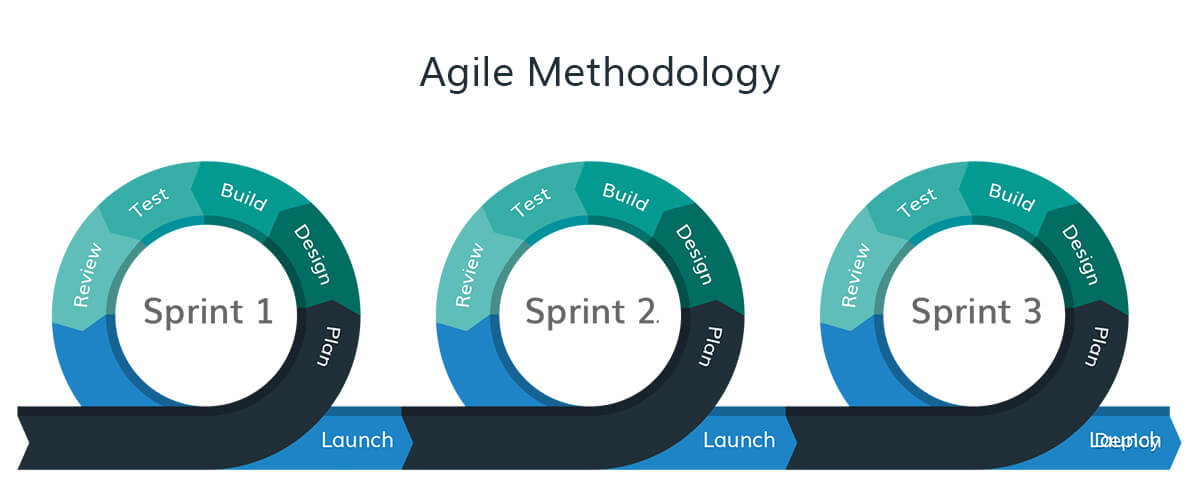
\includegraphics[width=0.7\textwidth]{final-year-project-template-master/img/agileSprint.jpg}
     \caption{Agile mythology for Project }
\end{figure}

    \subsection{ Development Environment  }
    
  The project was developed using Android Studio. The software has a wide suite of tools for testing, developing, and deploying. One large benefit is the built-in android emulator to deploy your application and see changes in real-time.Although this environment was new to me, given the Android emulator  and the feature-rich coding environment. I felt it would provide enough functionality to successfully create my android application.
    
    

    \subsection{ Setting Objectives   }
    
By Implementing an agile methodology,objectives were set by  week. Through the GitHub  web interface  I  created an  agile storyboard as shown below:
    
    
       \begin{figure}[H]
  \centering
    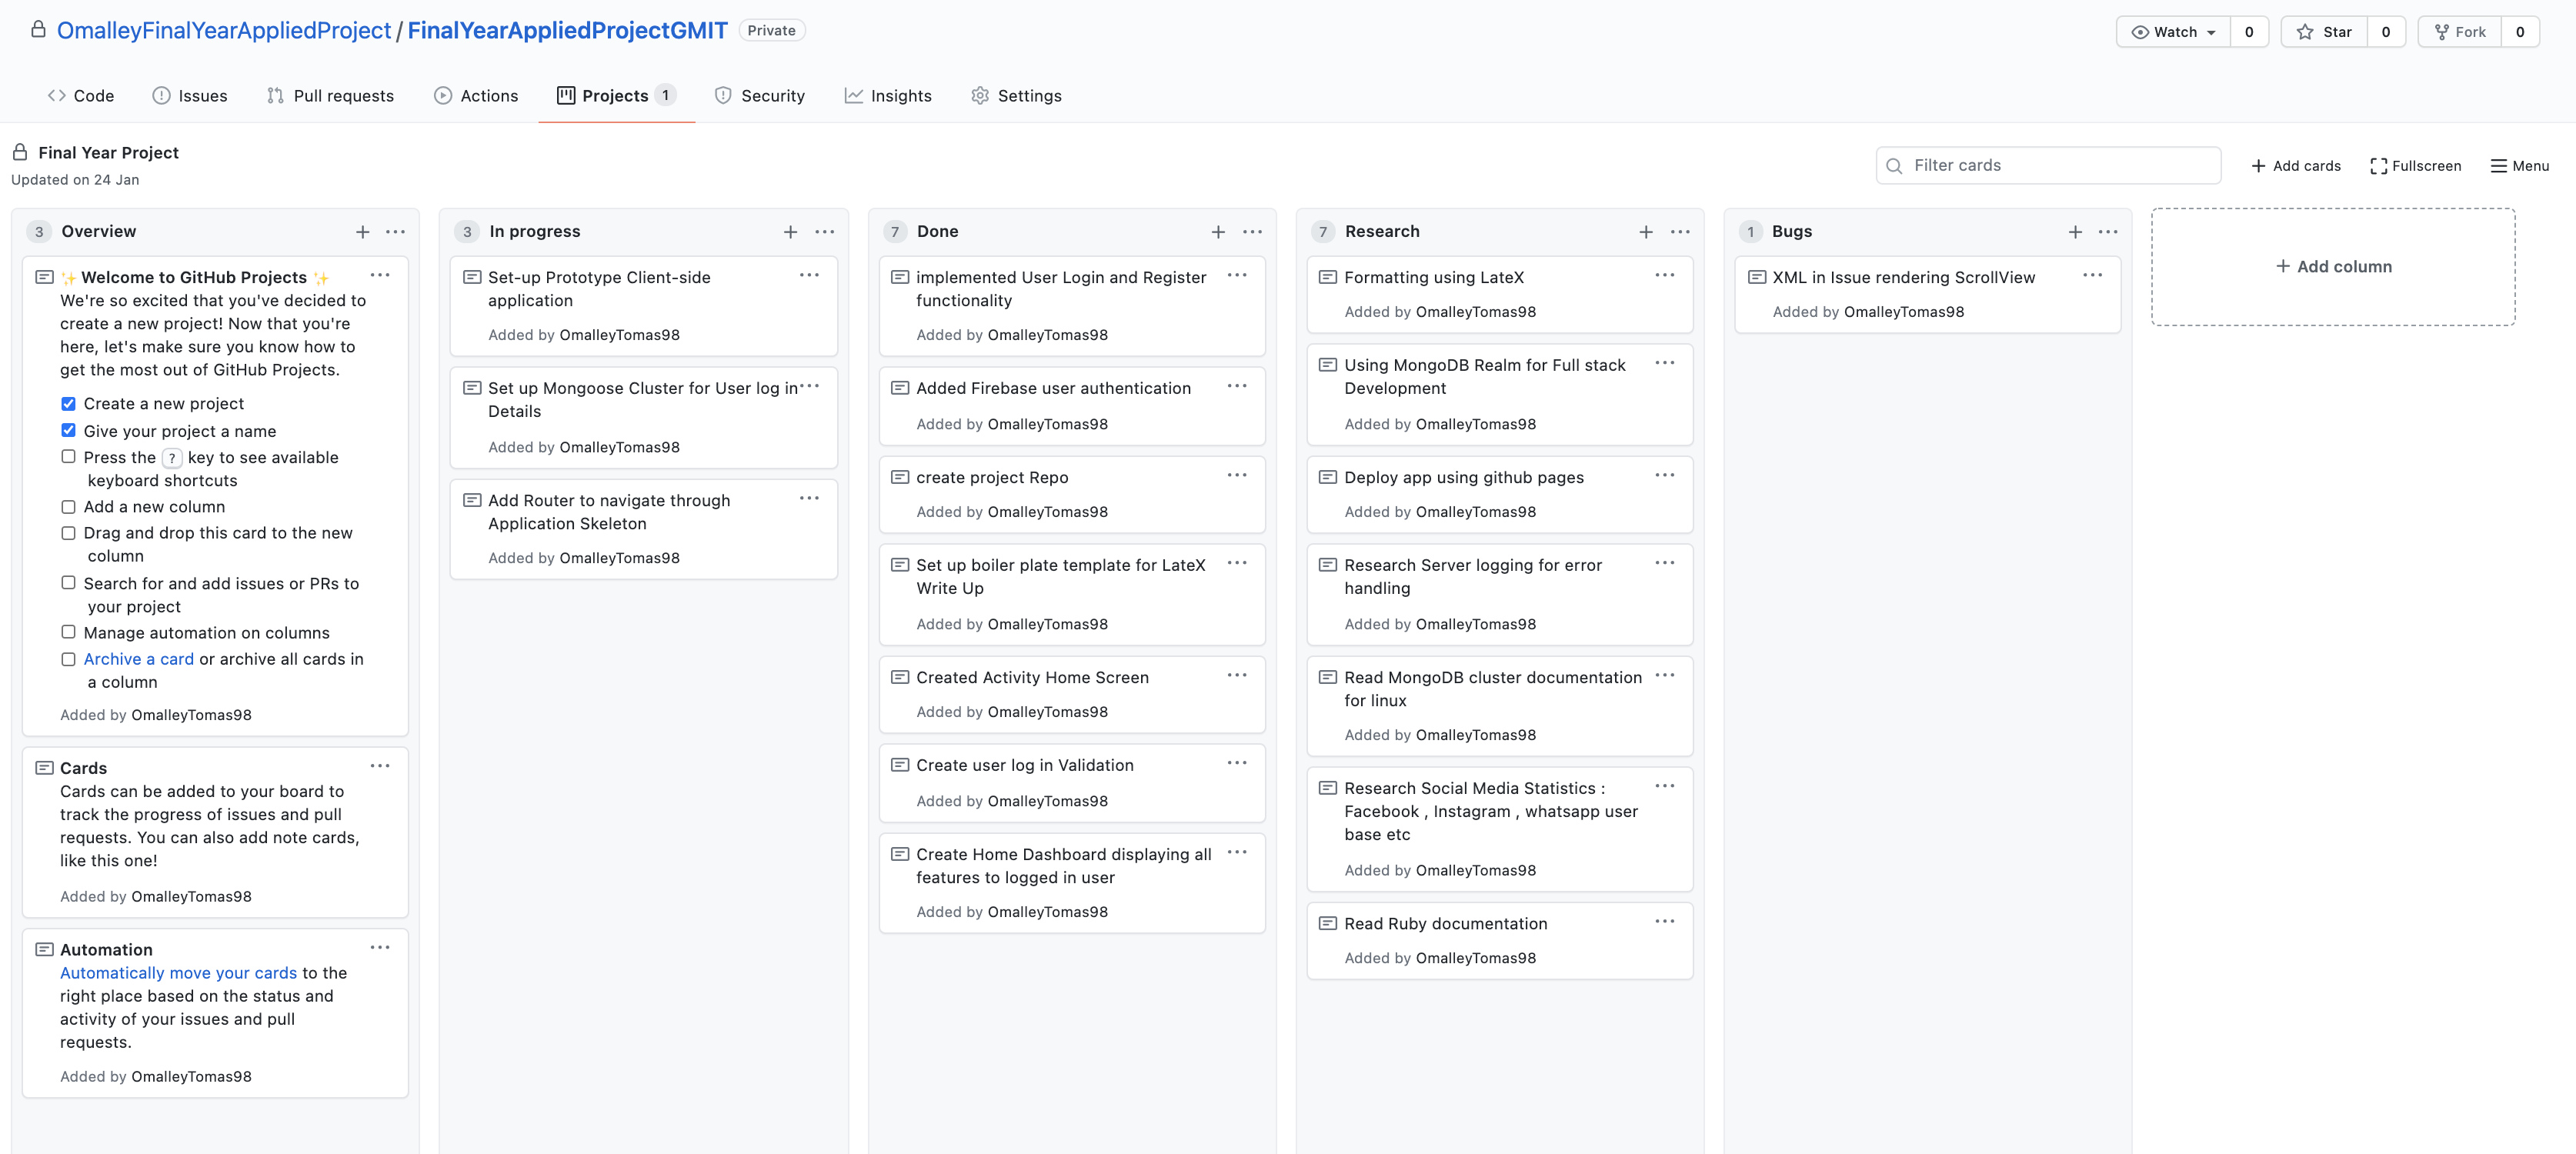
\includegraphics[width=1.0\textwidth]{final-year-project-template-master/img/storyboard.png}
     \caption{Story Board }
\end{figure}


    I created the storyboard and added each task depending on  whether the  task was complete or still under development to keep track of my progress.The following list of objectives required for the project were outlined as follows:
    
    
    
    
    
    
     \begin{figure}[H]
  \centering
    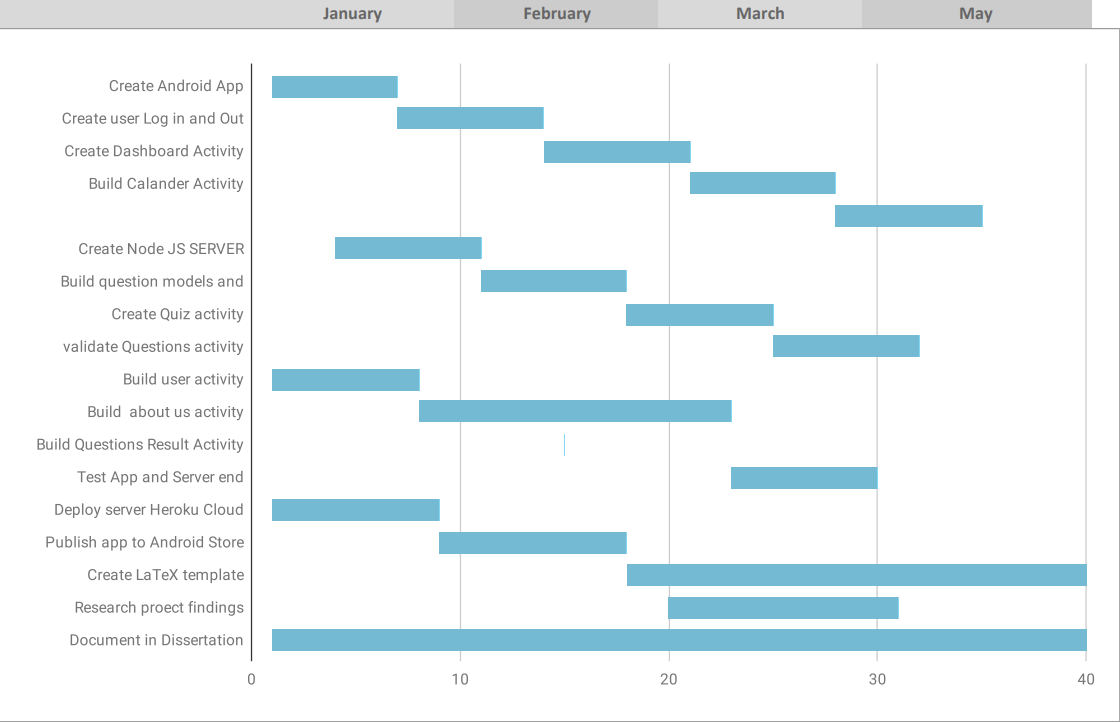
\includegraphics[width=1.0\textwidth]{final-year-project-template-master/img/GanttChart.png}
     \caption{Sprint Gantt Chart }
     
    As displayed in Fig3.4 above, a Gantt chart of activities was created outlining a timeline for each activity. The chart was created using google docs (free to use online document editor). Because the project was solo, a collaborative tool or spaces offered by other platforms such as click-up or Asana were not required.
    
    
    \\Prior to beginning development on the project, the following steps would be required so that I would be familiar with the environment and language as the project progressed
    
     
     
\end{figure}
    
    \begin{itemize}
  \item  Explore Android Mobile Development. 
  \item  Study the Kotlin language.
  \item  Research online effectively through peer-reviewed articles and  other content  to review Software Development. 
\end{itemize}
    
    
    
            \subsection{ Strategy Software }
            Following  are the different types of software that helped communicate and shape the criteria for my final year project.


 \begin{itemize}
     \item \textbf{Microsoft Teams:} A communications team management tool developed by Microsoft as part of the Microsoft Office  365 software suite. Galway Mayo Institute of Technology currently uses this software for streaming live lectures during  the COVID-19 pandemic.MS teams also allow for private messaging, file transfer and is available for   Windows, Mac, Web and mobile platforms which is an advantage to other collaboration applications.

         \end{itemize}
         
          \begin{figure}[H]
  \centering
    
\includegraphics[width=0.2\textwidth]{final-year-project-template-master/img/msteams.png}
     \caption{Microsoft Teams Icon }
\end{figure}

    
        \subsection{Meetings}
        My Supervisor organized a weekly catch-up via the Microsoft Teams platform as an alternative to on-campus meetings due to the temporary closure of the campus in line with government regulations. Each week I demonstrated my work and I received feedback on the architecture, complexity, and what milestone will be delivered next on my agenda. Examples of topics discussed in my meetings: 
        
\begin{itemize}
 \item The scope of features. 
 \item Discussion on known issues or limitations.
 \item How the feature interacts with the application.
 \item General Feedback on project quality.
 \item Review of current application.
 \item Delegate tasks to be completed before next meeting.
 
 It was key for the progression of my application to discuss whether the components were to the correct scope and to create points for iterative development each week.

\end{itemize}

    \subsection{Testing approach}
When testing an application there are a variety of  approaches and benefits. Testing is vital to create a solid well-optimized application. Following are the two main forms of testing used in my project

\begin{itemize}
\item  \textbf{Black Box testing:} Black box testing is an approach to evaluating the quality without the tester having access to the working internals. I found the black box approach appropriate when testing my application from the perspective of a user. 

\item  \textbf{White Box testing:} White box testing is an approach where the tester has an understanding of programming fundamentals with access to the internal code to create dissected tests to evaluate the quality and ability of the application. White box testing was highly beneficial for testing my application features, I designed an array of test cases as described in section 3.0.7  


\end{itemize}


\textbf{Example testing  criteria  of project:}


\begin{itemize}
\item Test if an e-learning application can be used on different mobile devices e.g Android KitKat, IceCream, etc.
\item Testing load speed of application on multiple Android Emulator APKs.
\item Add User to Firebase DB.
\item Create User Model.
\item Test speed of Get and Post  Request using OKHTTP Client.
\item Test speed of Android view list vs recycle view for loading data on  screen.

\end{itemize}

When testing my mobile Application I  implemented the Testing Pyramid. The pyramid is an industry-grade guideline due to its simplicity and practicality, as outlined below:

\begin{enumerate}
  \item \textbf{End to End testing:} A test on the applications workflow , Replicates real user scenarios.
  \item \textbf{Integration Testing:} A  test  where software modules are integrated logically and tested as a group.
  \item \textbf{Unit Testing:} A Testing is the process of checking small pieces of code to deliver information early and often.I found this approachable improved the quality of my application and prevented integration issues.
\end{enumerate}

\begin{figure}[H]
  \centering
    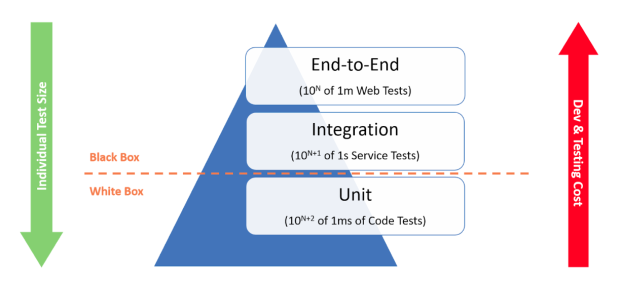
\includegraphics[width=0.8\textwidth]{final-year-project-template-master/img/testingpyramid.png}
     \caption{Testing pyramid }
\end{figure}

I created a number of unit tests orientated around the applications features which are in detail in Section 6.0.2.


\chapter{Technology Review}

\subsection{Kotlin}
Kotlin is a cross-platform, statically typed, general-purpose programming language with type inference. Kotlin is designed to interoperate fully with Java, and the JVM version of Kotlin's standard library depends on the Java Class Library. As of 2018 Kotlin holds a 25.30 percent market share among the top apps\cite{kotlinstats}.I chose Kotlin due to its close syntax to Java and its rich documentation.Jet-brains, the creators of the Android Studio IDE provide a tool to convert Java code to Kotlin code.Kotlin is a suitable  choice for solving challenging design problems and ensures further support than legacy java programs.



The front-end of the application refers to  The layer above the back end is the front end and it includes all software or hardware that is part of a user interface. Human or digital users interact directly with various aspects of the front end of a program.The front-end of this application is written in Kotlin.


 
 \begin{lstlisting}[language=Java, caption= Java vs Kotlin code Snippet ]
// Java code snippet
public void createAndPrintMessage(){
    String title = "Java Example";
    Message message = new Message(title);
    printMessage(message.getMessage());
    }
}
// Kotlin Code Snippet
fun createAndPrintMessage(){
    val title = "Kotlin Example"
    val message = new Message(title)
    printMessage(message.title)
}
 \end{lstlisting}



\subsection{Node JS} 
The Back-end of the application refers to parts of a computer application or a program's code that allow it to operate and that cannot be accessed by a user.
Node.js is built on the  V8 JavaScript engine. After initialy experimenting with various  server-side languages such as ruby n rails I settled on node js due to its extensive documentation,support base strength in building light web servers.



\subsection{MongoDB}
MongoDB is a general-purpose, document-based, distributed database built for modern application developers and for the cloud era\cite{mongodocs}.   

I implemented MongoDB using the atlas feature.MongoDB Atlas is a  free  database service . I choose an AWS machine based in the EU to help with latency issues. A  benefit to using MongoDB is its web-based graphical user interface. MongoDB allows you to display databases as clusters and add records directly through the browser.MongoDB holds all the quizzes and questions used for my learning application. I chose MongoDB due to its vast popularity with web applications and its extensive documentation.



\begin{figure}[H]
  \centering
    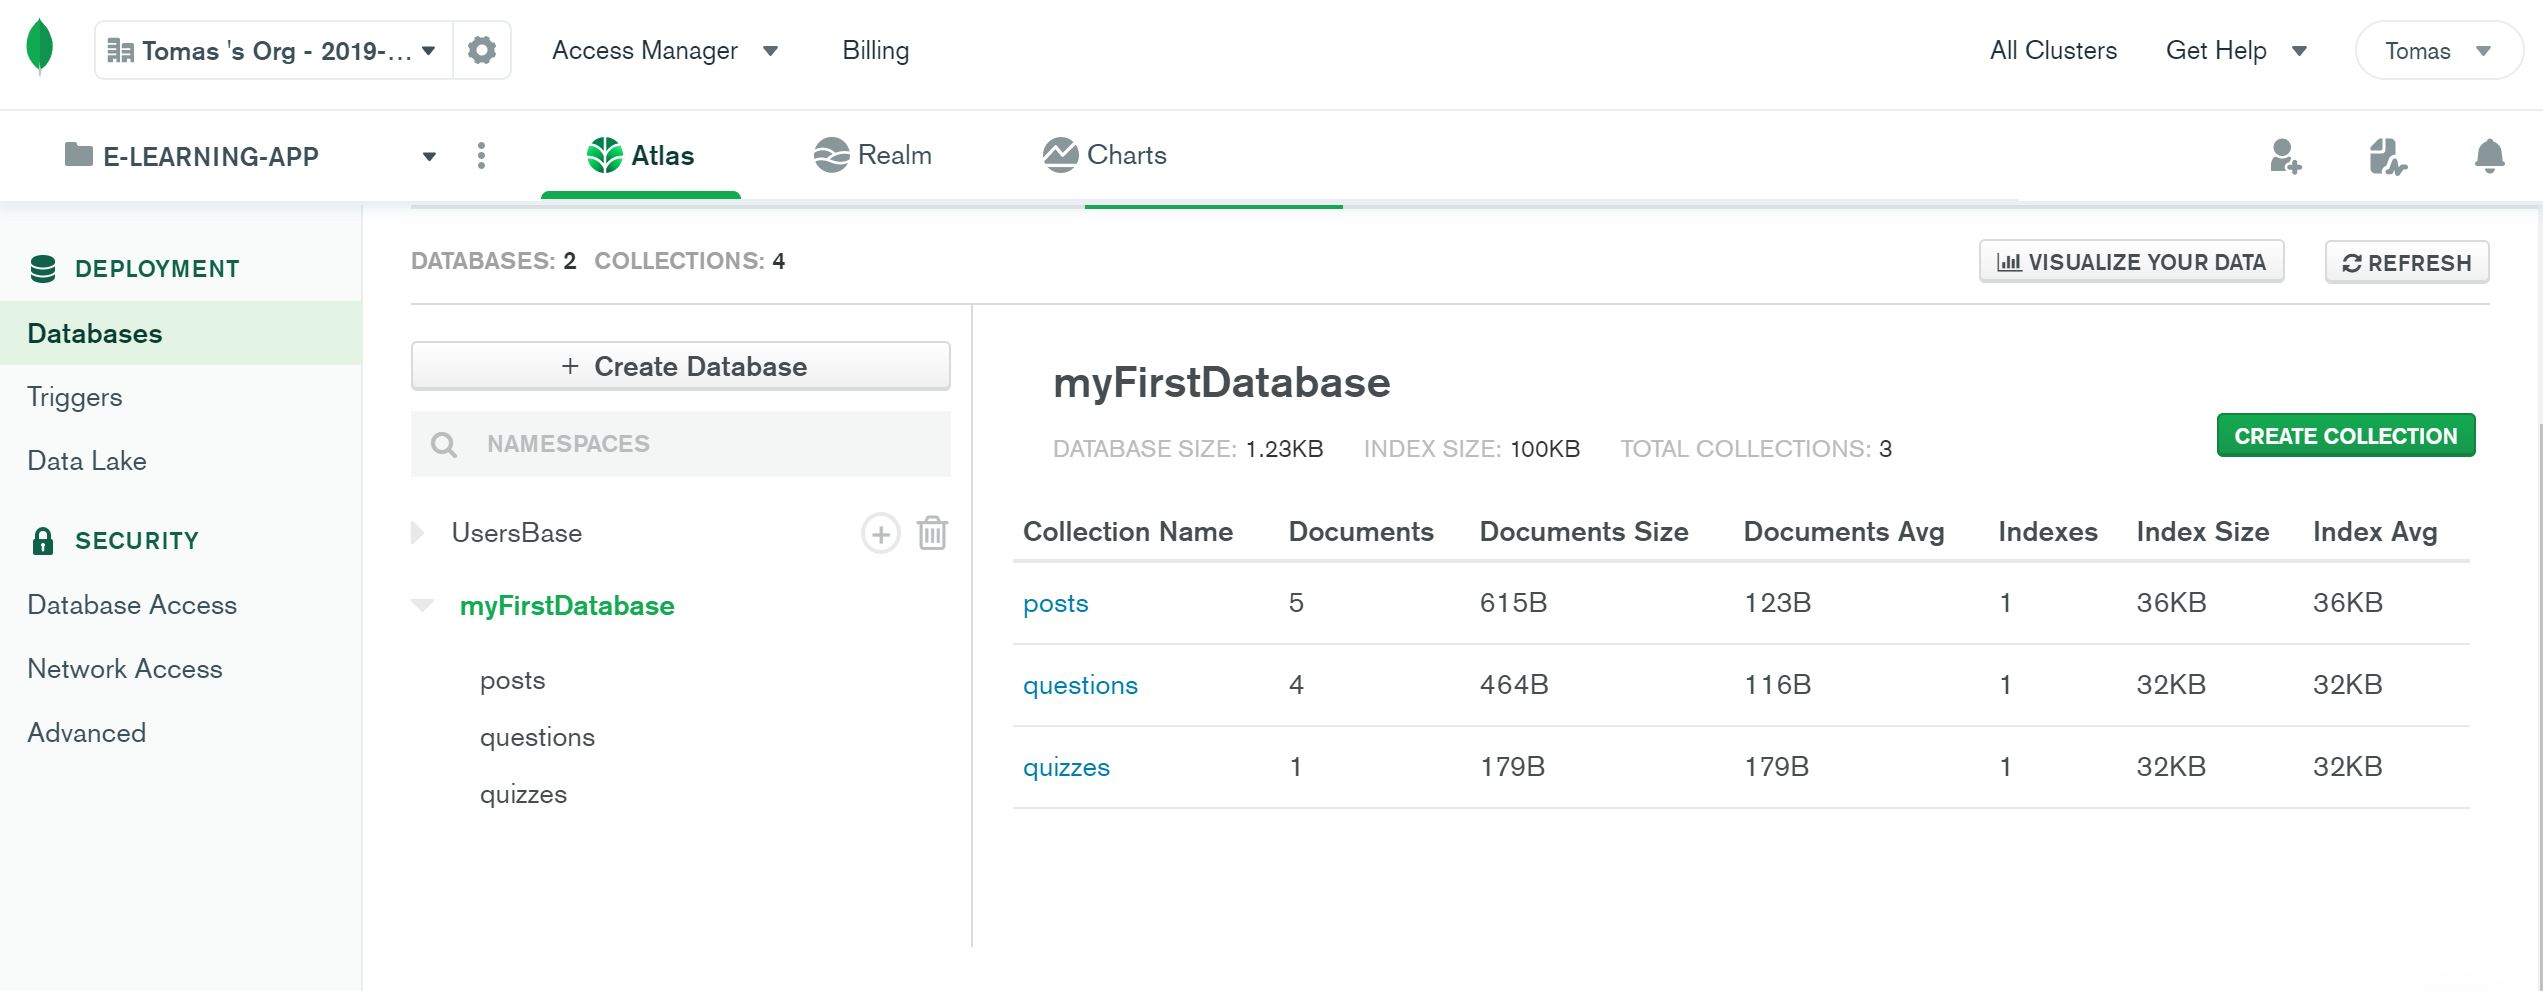
\includegraphics[width=1.0\textwidth]{final-year-project-template-master/img/myMongoCluster.JPG}
     \caption{MongoDB Cluster }
\end{figure}




\subsection{Firebase Authentication} 

Firebase Authentication provides back-end services,  SDKs, and ready-made UI libraries to authenticate users to applications \cite{firebaseauth}. It supports authentication using passwords, phone numbers, popular federated identity providers like Google, Facebook and Twitter, and more. I chose Firebase due to its  performance for Android and along with  the detailed documentation provided by Google. Firebase providers developers with a Graphical User interface to view a list of permissions and users.


\begin{figure}[H]
  \centering
    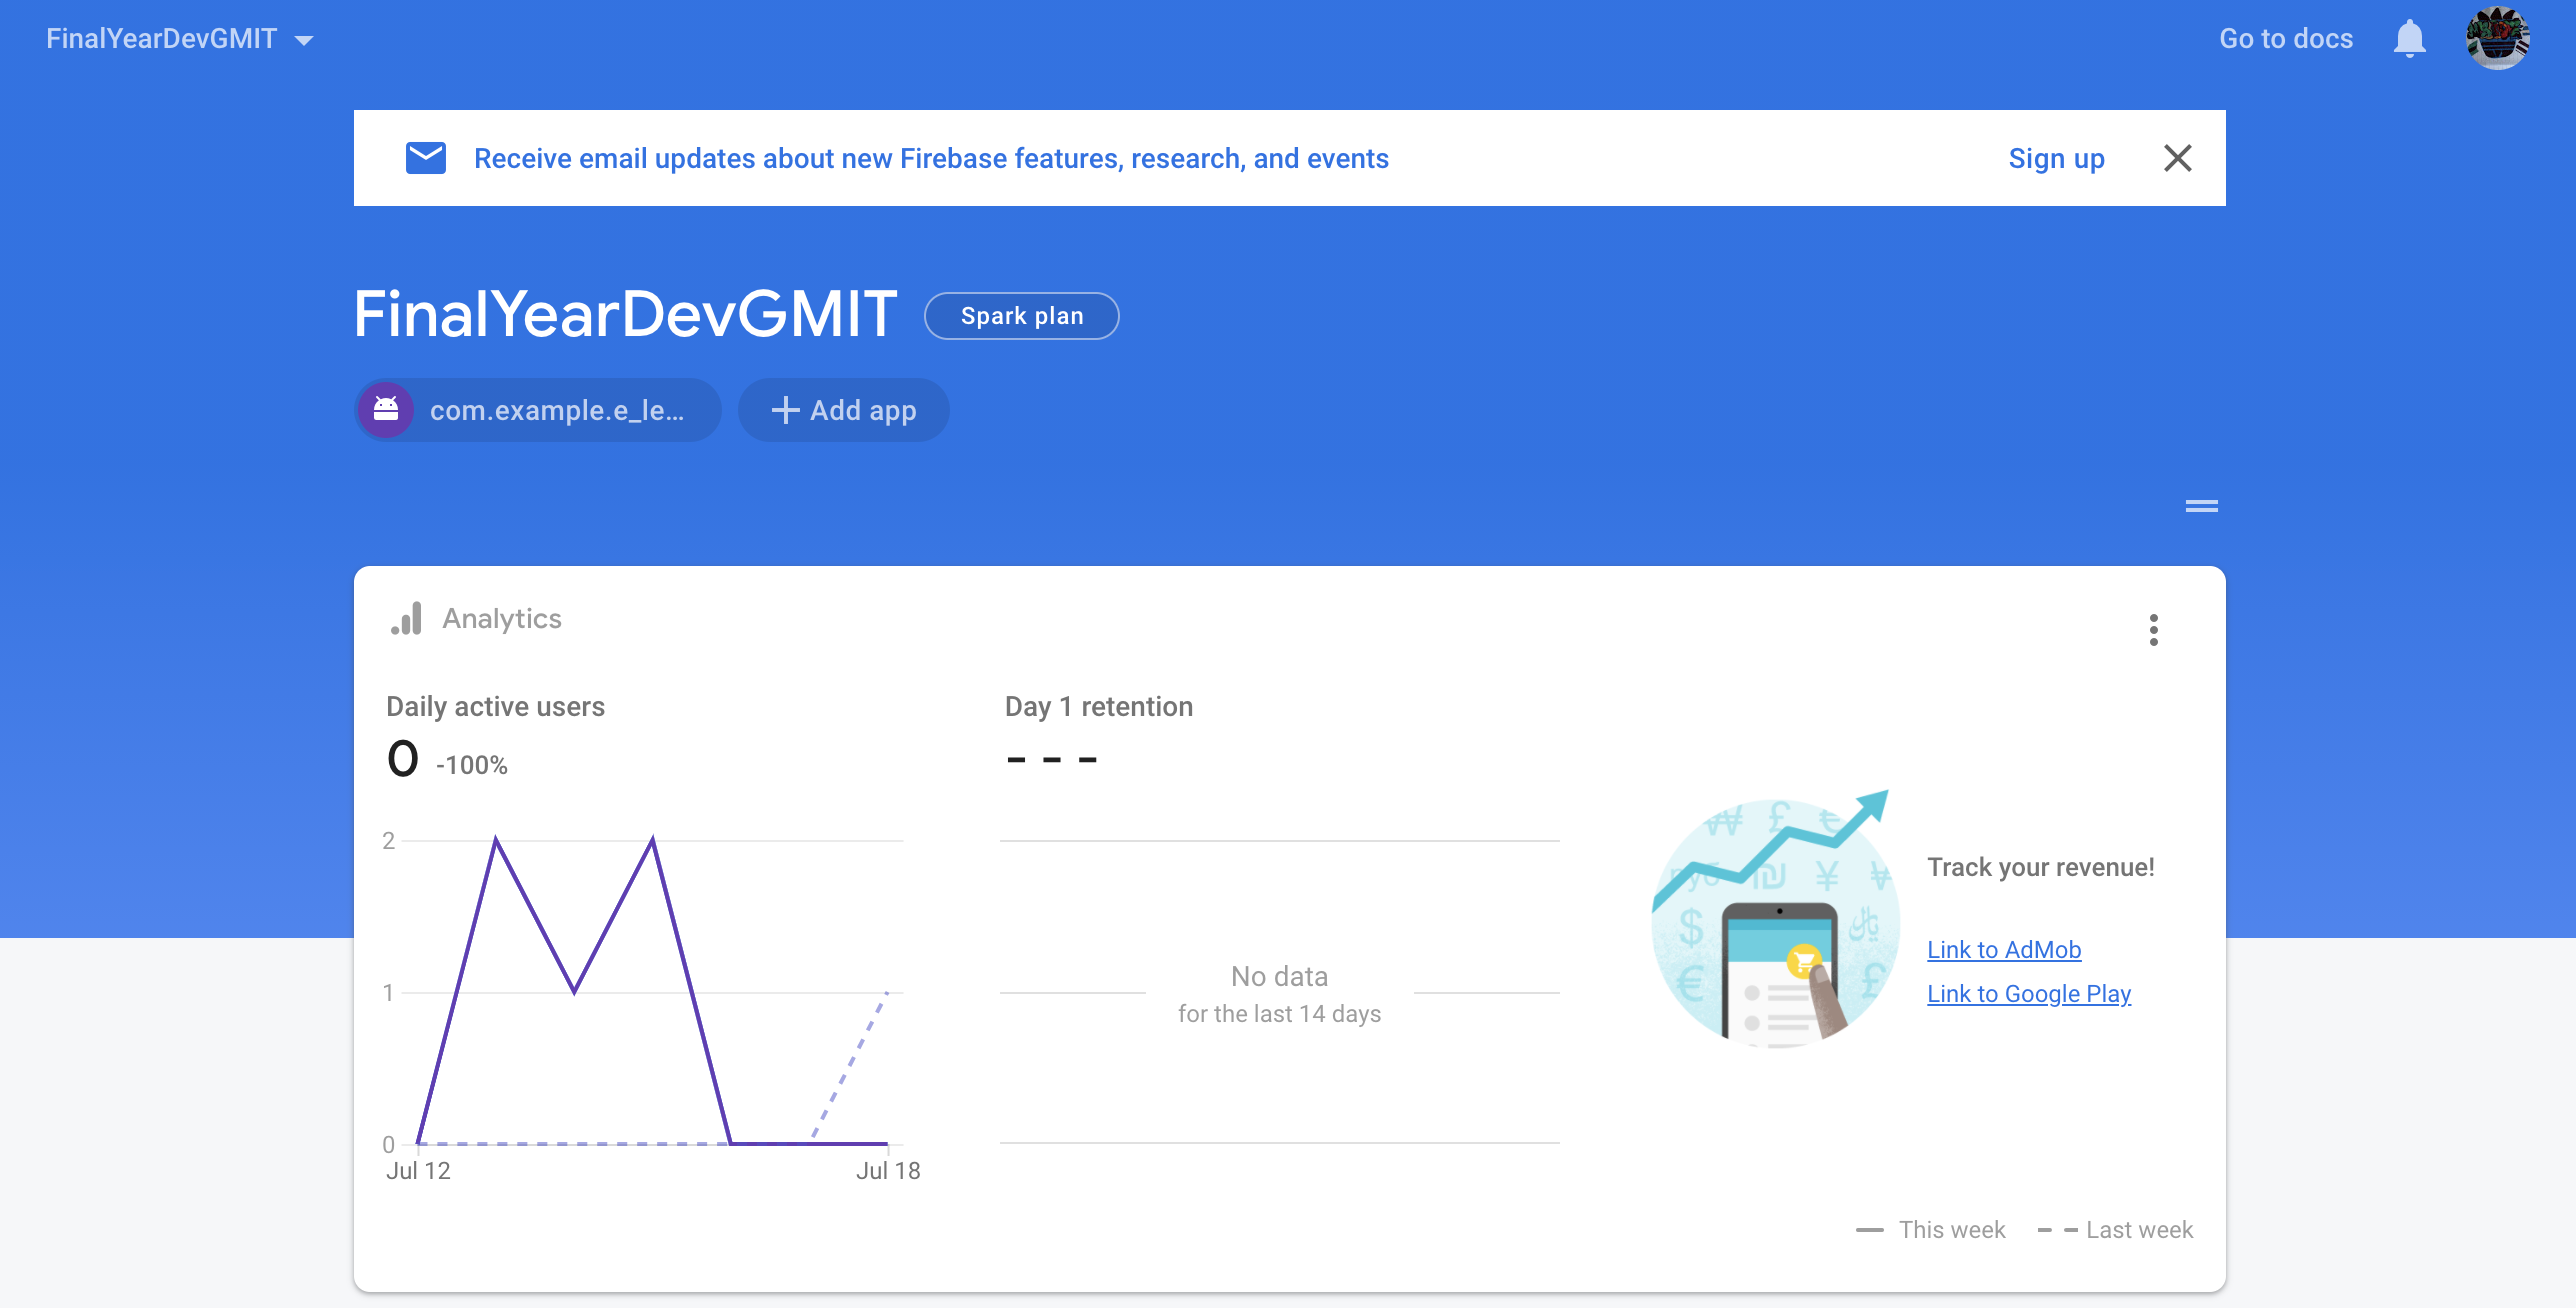
\includegraphics[width=1.0\textwidth]{final-year-project-template-master/img/firebaseconsole.png}
     \caption{Firebase Development Console}
\end{figure}




\subsection{SQLite Database }

When focusing on users data, I chose to integrate a simple local database system  commonly found on android devices for storing local data, as  opposed to storing
the data in my MongoDB Database.This  simple system stores the users data events in the Calendar activity.This feature was  integrated  so that  users may can access their events while offline.SQLite is a   lightweight , responsive and  robust storage system which was perfect for providing a smooth experience for the end user for the purposes of this applciation.


\subsection{XML Styling} 
Extensible Markup Language (XML) is a markup language that defines a set of rules for encoding documents in a format that is both human-readable and machine-readable. I chose XML  as its easily read structure and strong integration with Kotlin.XML offers  freedom from styling separate items to creating  uniform styling for components. I created a simple style sheet to provide a clean and consistent style for users. Both Apple and Android provide Human interface guidelines\cite{styleguidelines} which proved useful in the design and function of the front end of the application. The guidelines provide specifics on how applications can attract end-users and indicate the most suitable styles to use for front-end elements such as icons, buttons and windows.



\subsection{Android Studio}
Android studio is a popular and widely  used IDE for creating android applications.Android studio is the official Integrated Development Environment (IDE) for Android OS\cite{androidstudio}, that can be deployed on Windows, MacOS and Linux operating systems.It is developed by both Google and JetBrains, and supports Java, C++ and Kotlin.


   \begin{figure}[H]
  \centering
    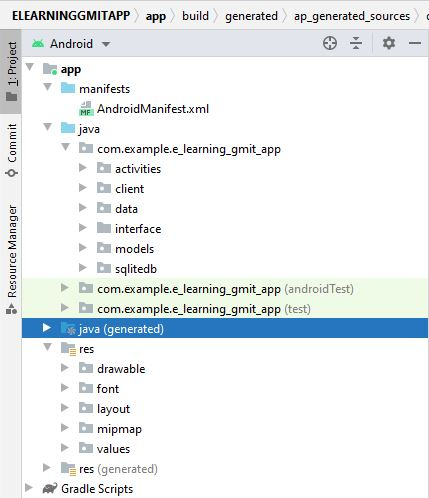
\includegraphics[width=0.35\textwidth]{final-year-project-template-master/img/codebase.JPG}
     \caption{Refactored Codebase in Anroid Studio IDE}
\end{figure}


   \begin{figure}[H]
  \centering
    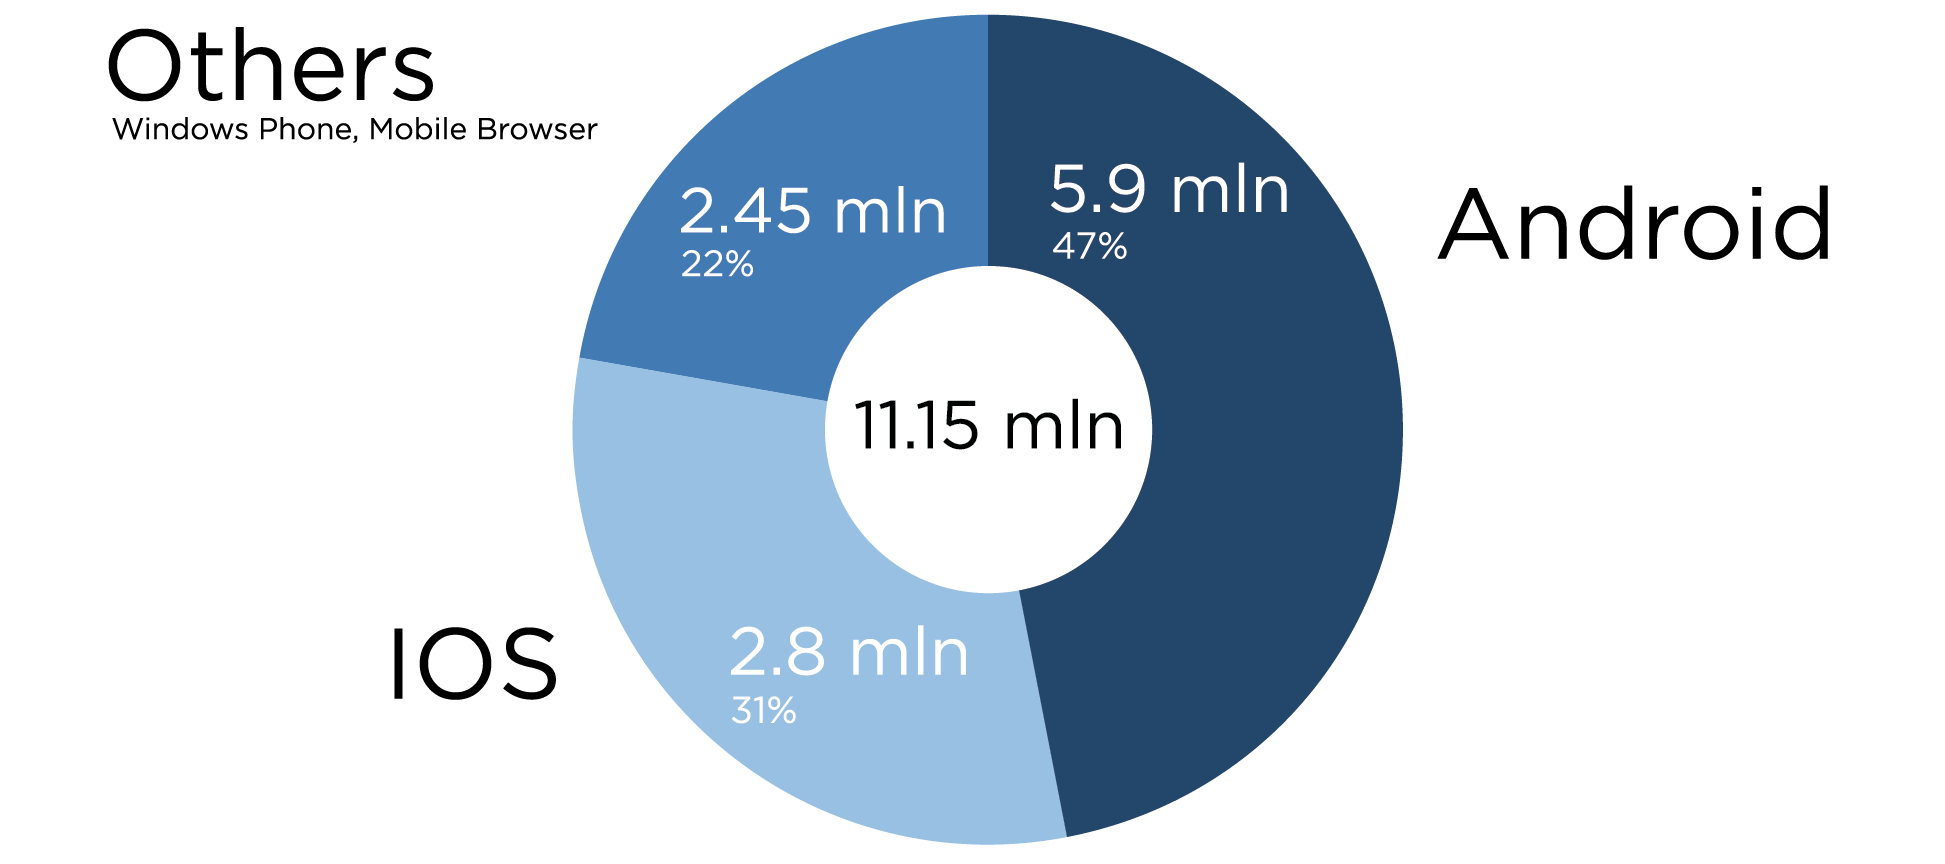
\includegraphics[width=0.7\textwidth]{final-year-project-template-master/img/marksetSHareAndroid.png}
     \caption{Android user base share}
\end{figure}

\subsection{Cloud Deployment}

After tackling the issues of locally stored data, I researched implementing cloud technologies. Cloud technologies are playing an increasingly important role for companies such as Microsoft and Amazon, with both providing their own cloud options. I had initially planned to use Microsoft’s Azure service, but found the options provided were not the most suitable for the type of application I was building. I then settled on the Heroku cloud application platforms \cite{herokucloud} which provides free environments, along with the core requirements I needed for my application, including: 


\begin{figure}[H]
  \centering
    
\includegraphics[width=0.35\textwidth]{final-year-project-template-master/img/heroku.png}
     \caption{Heroku Logo}
\end{figure}

Pros of Heroku Cloud Deployment
\begin{itemize}
  \item   \textbf{Pricing:}
 Other provides such as AWS provide less competitive pricing per virtual machines 
  \item \textbf{Ease of use:}.  Heroku proceeds strong integration alongside GitHub with a dashboard 
\end{itemize}


As shown in fig 3.3 Heroku is consistently growing in popularity over the popular competitor 
Amazon web services\cite{herokuawsstat}. A  benefit of Heroku  its strong link to git, I found Heroku online documentation  straightforward and it helped me  to deploy my application to the cloud.

   \begin{figure}[H]
  \centering
     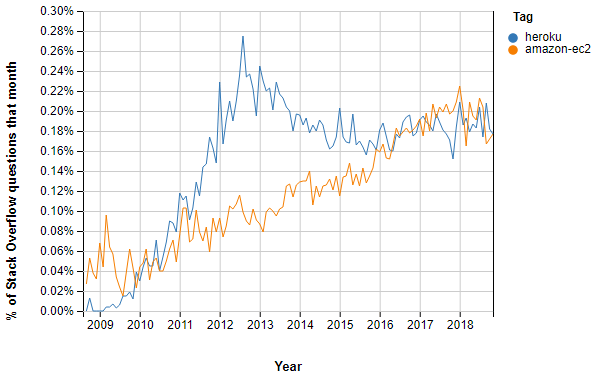
\includegraphics[width=0.8\textwidth]{final-year-project-template-master/img/herokustatistics.png}
     \caption{Popularity in cloud services }
\end{figure}

Heroku provides a friendly website dashboard that lists all current apps and the number of commits of the deployed service.

\begin{figure}[H]
  \centering
    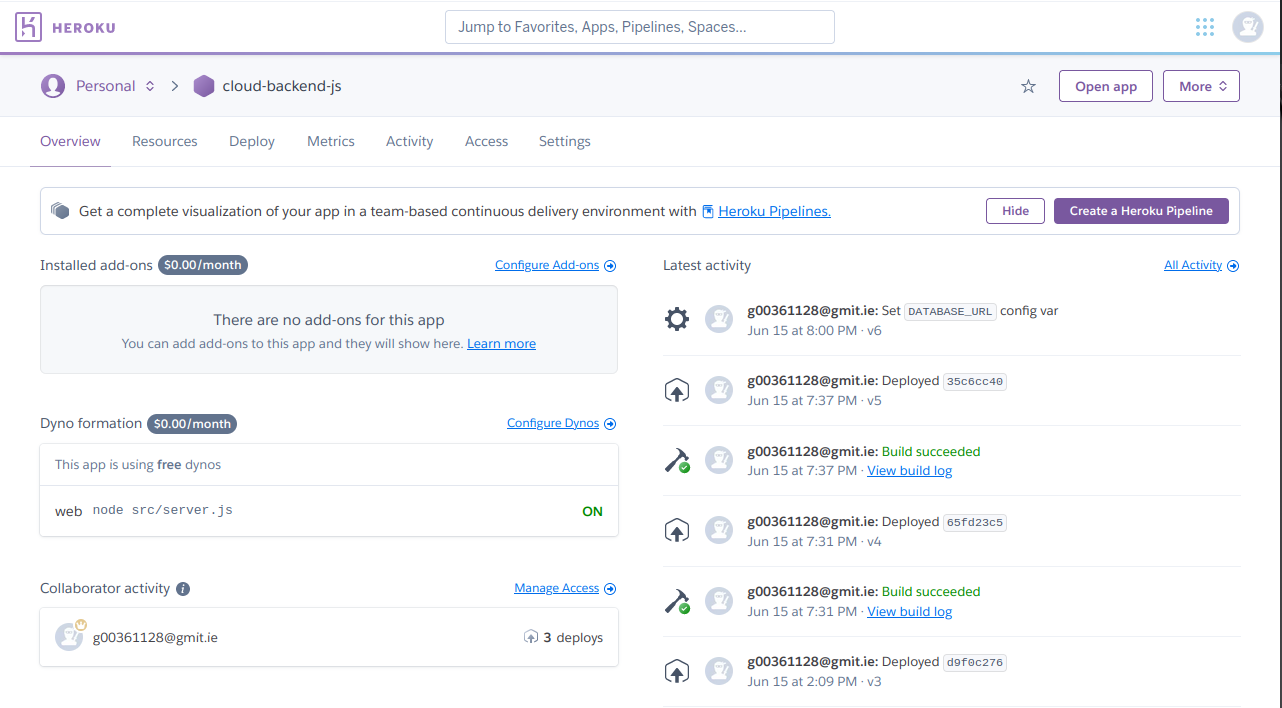
\includegraphics[width=0.8\textwidth]{final-year-project-template-master/img/herokuDashboard.png}
     \caption{Heroku  dashboard }
\end{figure}


\subsection{Android Emulator}

The Android Emulator simulates Android devices on your computer so that you can test your application on a variety of devices and Android API levels without needing to have each physical device. The emulator provides almost all of the capabilities of a real android device. The android emulator is an extremely effective tool for deploying an android app without having physical hardware. The android emulator used is shown in the figure below. 

\textbf{Pros of Android Emulator} 
\begin{itemize}
  \item \textbf{Integration:} Android Studio has strong integration with the Android studio integrated development environment.
  
 \item \textbf{Ease of use:}  Android studio is  easy to run. The APK is loaded without the developer and little to no documentation needs to be read.
  
   \item \textbf{Cost Effective:}  The Android emulator is free to use while buying a handset can be expensive.
   
    \item \textbf{Variety:} The built-in Android emulator packaged with IntelliJ comes with a wide variety of different types of flagship Android devices to test.
\end{itemize}


\begin{figure}[H]
    \centering
    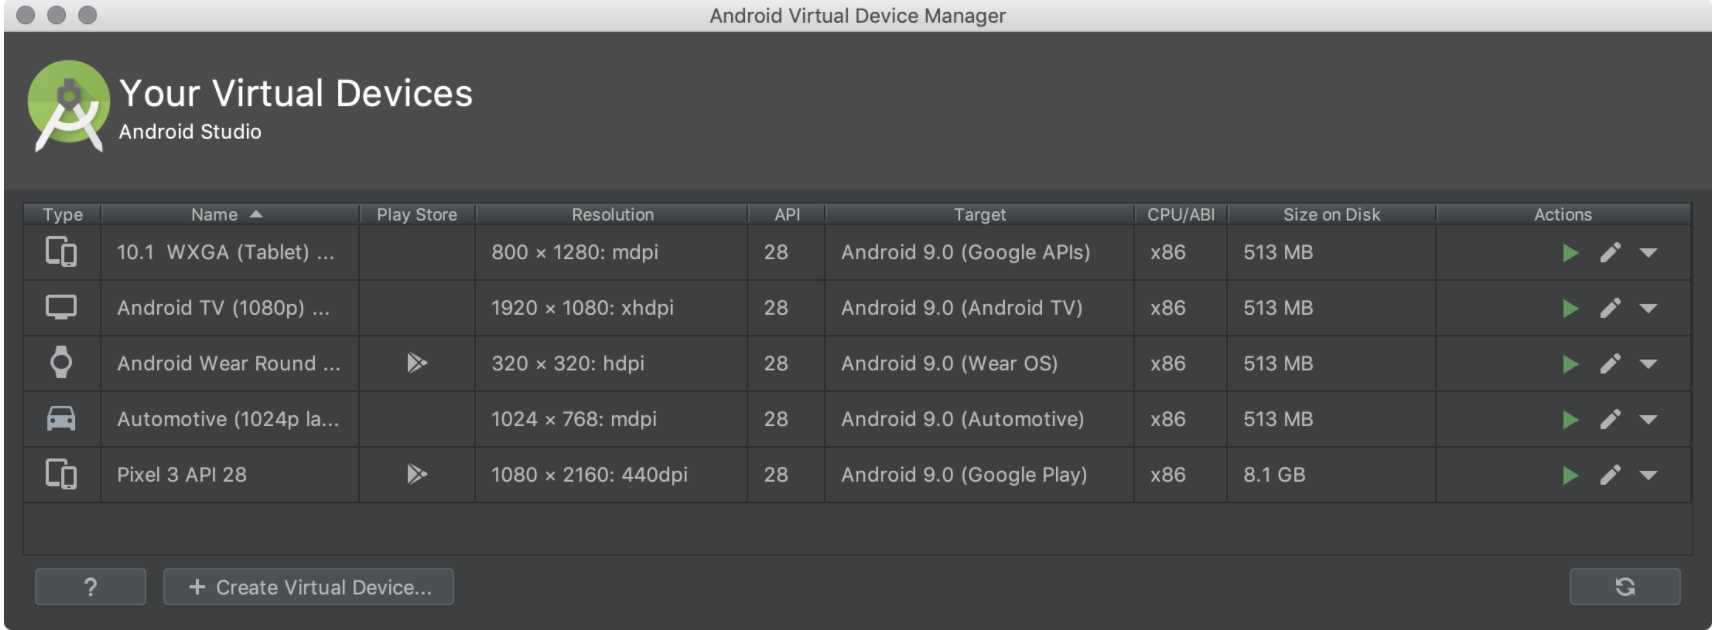
\includegraphics[width=9cm]{final-year-project-template-master/img/AndroidAVDManager.png}
    \caption{Android AVD Manager displaying all available devices}
    \label{fig:Android AVD Manager}
\end{figure}



\subsection{Visual Studio code editor}
Visual Studio Code is a freeware source-code editor made by Microsoft for Windows, Linux, and MacOS. Features include support for debugging, syntax highlighting, intelligent code completion, snippets, code refactoring, and embedded Git. I choose Visual  Studio code due to its strong link with Windows, Linux, and macOS.A  positive feature is  Windows Subsystem for Linux (WSL) which allows developers to run a bash Linux terminal locally on their Windows machine and open its file system directly on their Windows development machine.  VS Code also has Github integrated at its root. 
 \begin{figure}[H]
  \centering
    
\includegraphics[width=0.2\textwidth]{final-year-project-template-master/img/studiocode.png}
     \caption{Visual Studio code icon}
\end{figure}



\subsection{Literature Software  Documentation}
For my dissertation, I used the LaTeX document preparation tool.
Latex is a typesetting system that provides various features for creating and writing high-quality documentation. After reviewing the online documentation I found it very straightforward to set up and discovered its various tool shortcuts. Latex can be installed locally on your personal computer or can be accessed using a web browser. I chose to use LaTeX through my browser website  (https://www.overleaf.com/) due to its ease of use. I decided to use latex as I had already used it with other projects and I was  impressed by the quality of the software as opposed to using other editors such as Microsoft Word.LaTeX was created in  the 1980s and allows for high-quality documents. I researched on the Overleaf website how to create tables, lists, charts,and other layout features. I used open-source packages to create graphics such as Question Pie charts, as illustrated in  Fig 1.1. Another writing tool I used while writing  Grammarly,which is  an online tool that reviews spelling, grammar, punctuation, clarity of languages.

 \begin{figure}[H]
  \centering
    
\includegraphics[width=0.2\textwidth]{final-year-project-template-master/img/overleaf.png}
     \caption{Overleaf }
\end{figure}


\chapter{System Design}

\subsection{Application Overview}
My application is composed of three primary components, an android mobile application for users to interact with, a database system for storing application information, and a server-side logic tier back-end.


  \begin{figure}[H]
  \centering
    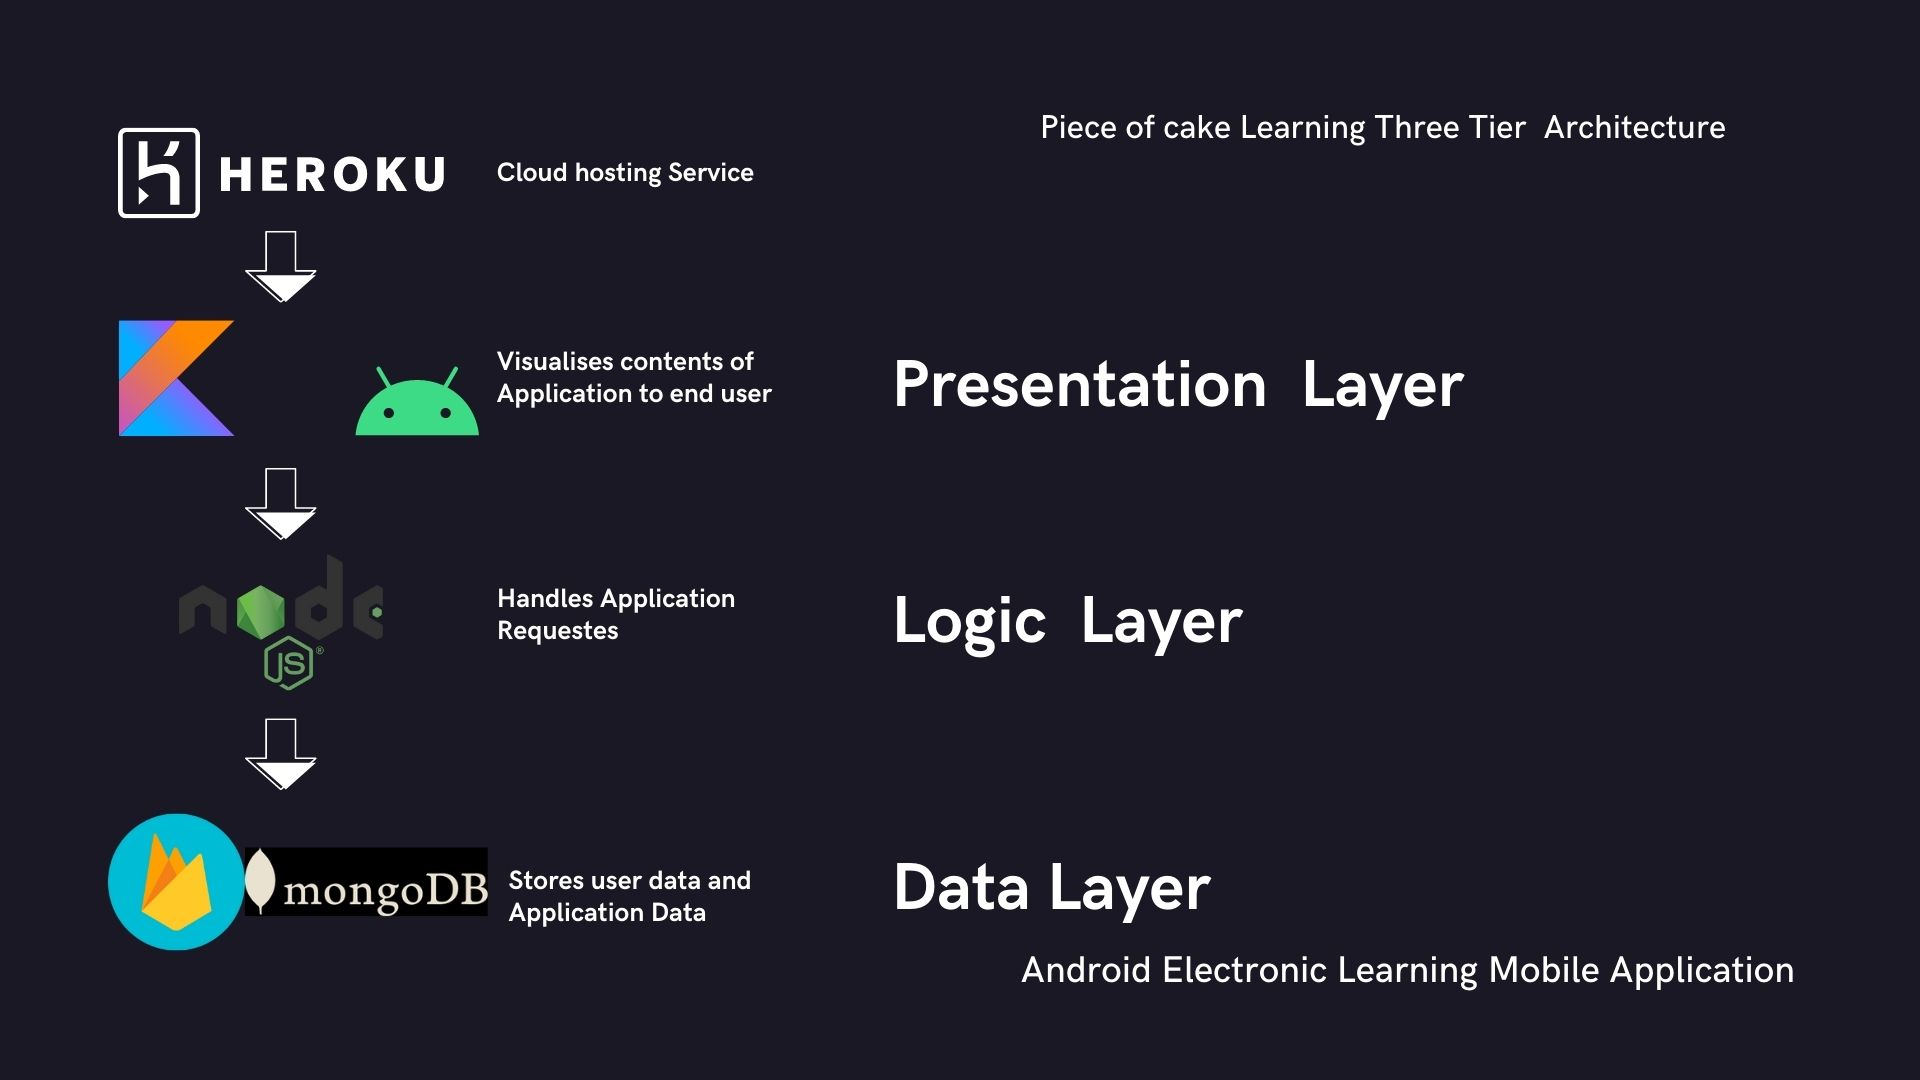
\includegraphics[width=0.9\textwidth]{final-year-project-template-master/img/designarch.jpg}
     \caption{Application overview}
\end{figure}

\subsection{Application Components}
Here I will break down all the components of the project.


\subsection{Gradle Build System}
Gradle is a build system used for creating applications such as mobile applications or web applications. Gradle essentially retrieves the apks from services to create apks for applications. Gradle is integrated with Kotlin Applications and all Android applications. The Gradle file is found in the active root of the Android application folder and is ran each time at compile. To implement different such as the OKHTTP client and Firebase authentication I had to follow the Documentation and import exactly else the application would stall with an error until edited.


\begin{lstlisting}[language=Java, caption=OKHTTP and Firebase imports in Build.Gradle]

    // quiz feed fot appi pull
    implementation 'com.squareup.okhttp3:okhttp:3.9.1'

    // Import the Firebase BoM
    implementation platform('com.google.firebase:firebase-bom:26.3.0')
    // Declare the dependency for the Firebase SDK for Google Analytics
    implementation 'com.google.firebase:firebase-analytics-ktx'

    \end{lstlisting}

    Gradle is a brilliant automation builder , it can provide detailed scans of the services being executed  and it is strongly supported by mainstream  IDES such as Android Studio , IntelliJ and NetBeans ( Java IDE ) . I gained experience working with the gradle build while creating a MVC Java Application for ... during third year using eclipse IDE. 

    
\subsection{Permissions}
To allow my android application to run correctly it must have permissions to allow networking features

\begin{lstlisting}[language=Xml, caption=Android Permissions]


<uses-permission android:name="android.
permission.INTERNET" />
    <uses-permission android:name="android.permission
    .ACCESS_NETWORK_STATE" />

\end{lstlisting}


\subsection{Application Style-sheet}
While developing the prototype for my application I settled on a set colour scheme for the application. As discussed in section 3.0.5 I used XML as a front end for styling my mobile application.I chose a green and white overall theme for styling the application.

\begin{lstlisting}[language=Xml, caption=App Stytlesheet]

<?xml version="1.0" encoding="utf-8"?>
<resources>
   <color name="colorPrimary">#5271ff</color>
    <color name="colorPrimaryDark">#000000</color>
    <color name="colorAccent">#11F6C0</color>
    <color name="white">#FFFFFF</color>
    <color name="black">#000000</color>
    <color name="colorLightGray">#9F9F9F</color>
    <color name="colorWhite">#FFFFFF</color>
    <color name="bachground">#282633</color>
    <color name="purple">#6f50c5</color>
    <color name="whiteText">#fdfbfc</color>
    <color name="goldtext">#e2c98a</color>
</resources>
\end{lstlisting}




\subsection{Splash Screen}
The application opens with a short animation displaying the name of the application alongside a load bar. All large applications, for example, Facebook, Twitter, and Instagram implement a splash screen before reaching the login screen. The splash-screen was created using XML and its intended use is to introduce the user to the background services such as OKHTTP and firebase running.

  \begin{figure}[H]
  \centering
  
    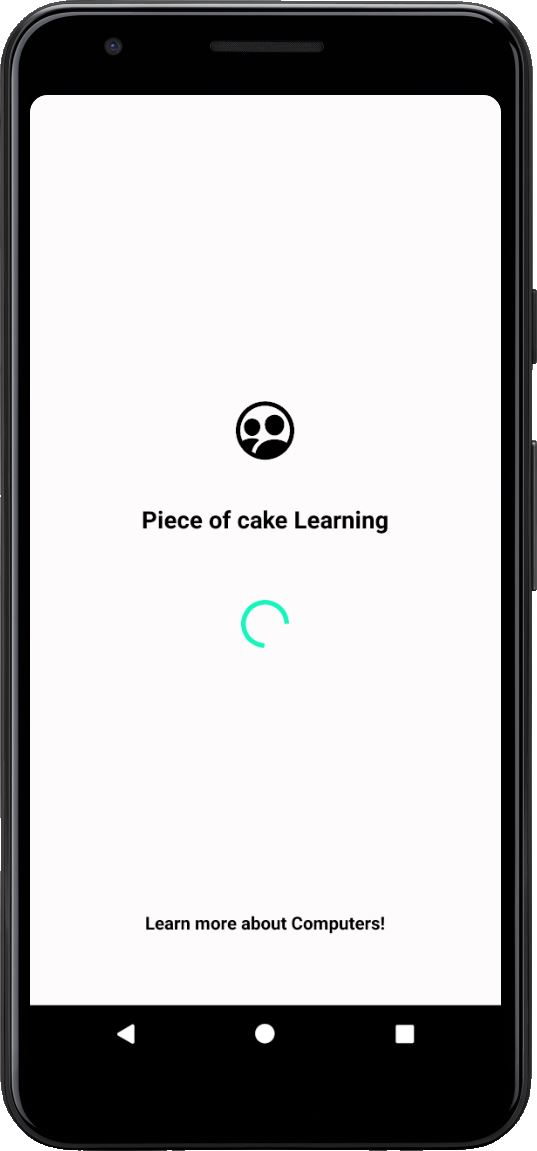
\includegraphics[width=0.35\textwidth]{final-year-project-template-master/img/finalsplashscreen.JPG}
     \caption{Android Splash Screen}
    \end{figure}
\lstinputlisting[language=XML ,caption= Code base for Splash screen]{codestubs/splashscreen.xml}



\begin{lstlisting}[language=Java, caption=Kotlin Splash Screen codebase ]

         private val SPLASH_TIME_OUT: Long = 3000 // 1 sec
  
        // Activity displayed in full screen
        window.decorView.systemUiVisibility = View.SYSTEM_UI_FLAG_FULLSCREEN
        Handler()
            .postDelayed(
                {
                    // This method will be executed once the timer is over
                    // Start your app main activity

                    startActivity(Intent(this, LoginActivity::class.java))

                    // close this activity
                    finish()
                },
                SPLASH_TIME_OUT
            )
    }

\end{lstlisting}
As shown in the codestubs in Listing 5.4 I implemented an image-view to display the logo , text view to display text and a progress-bar.Android provide a public progressbar method  which helped save me time from creating a rendered bar.Displayed in listing 5.5 , the progress is hard coded to display for 3 seconds before ending and the user is transferred to the sign in page using the StartActivity() method.



\subsection{Log In Register}
For the user to join the quiz lobby they must already create an account. The users' credentials are securely stored and verified using the Google Firebase API in Kotlin. The user interface is created using Kotlin and the XML markdown language. The user must enter their registered correct email and password to successfully log in. The user can log in three different ways.


\begin{enumerate}
  \item \textbf{Google Account:}Through the use of API the user can directly login or sign up using their Gmail account.
  \item \textbf{Facebook:}The user can sign in using their social media account on Facebook. To add this support I had to create a Facebook and link my application. Facebook provides detailed documentation on how to successfully implement the API.
  
  \begin{figure}[H]
  \centering
    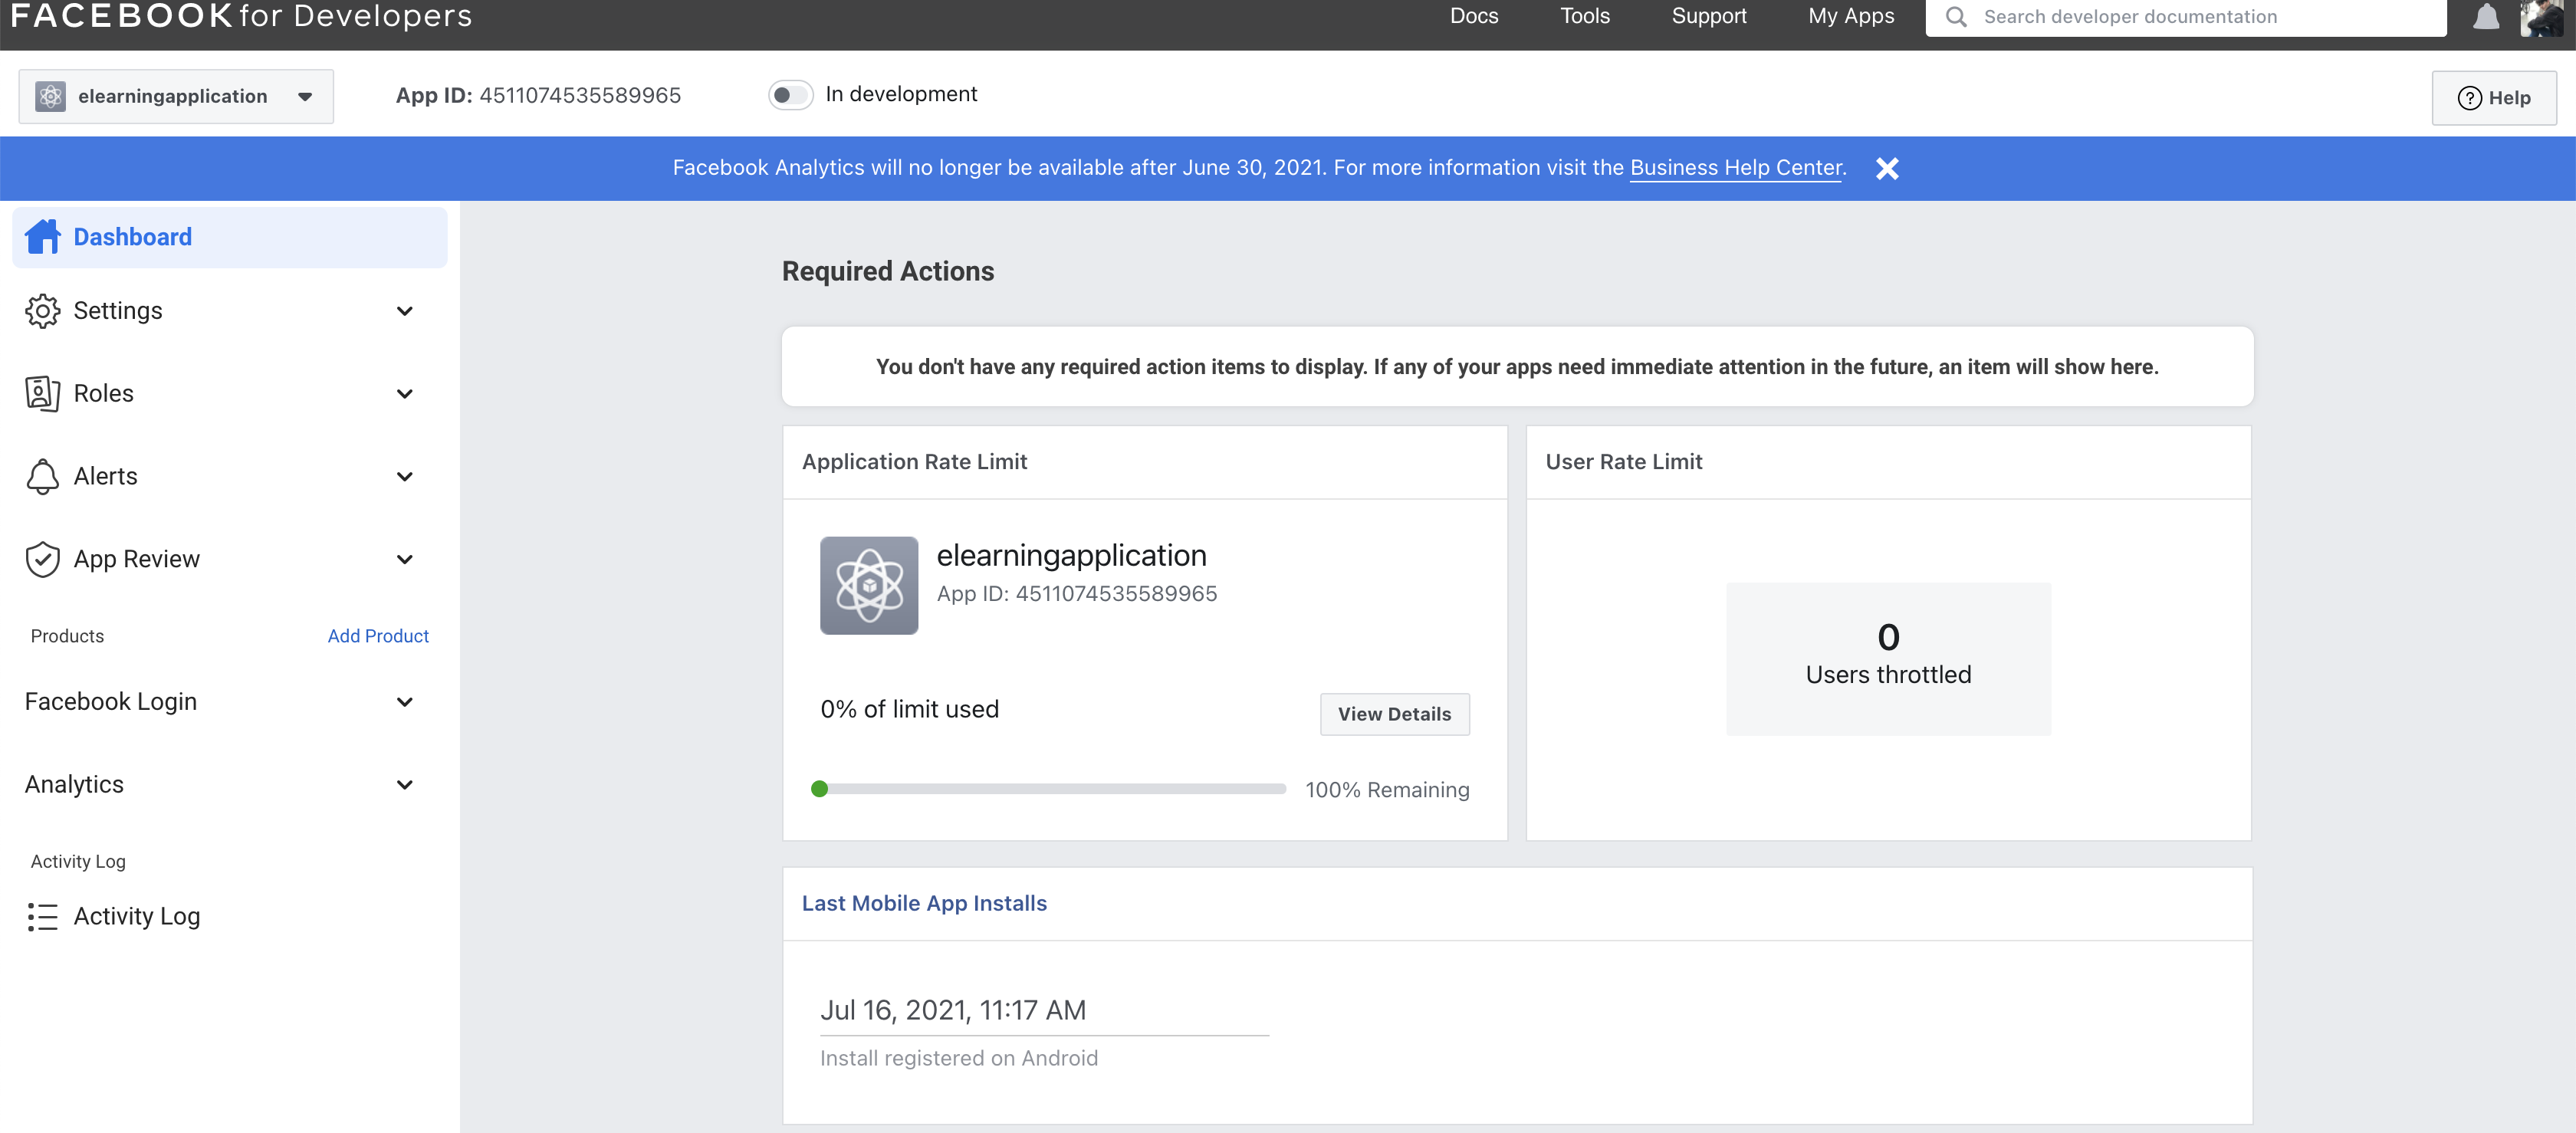
\includegraphics[width=0.8\textwidth]{final-year-project-template-master/img/facebookapi.png}
     \caption{Facebook Developers Homepage}
\end{figure}



Here are the methods I implemented to allow for Facebook authentication.

\begin{lstlisting}[language=Java, caption=Facebook Login /Sign up ]

    private fun facebookSignIn() {


        facebook_sign_in.registerCallback(callbackManager, object : FacebookCallback<LoginResult> {
            override fun onSuccess(result: LoginResult?) {

                handleFacebookAccessToken(result!!.accessToken)
            }

            override fun onCancel() {
            }

            override fun onError(error: FacebookException?) {
            }
        })
    }

    private fun handleFacebookAccessToken(accessToken: AccessToken?) {
        var credential = FacebookAuthProvider.getCredential(accessToken!!.token)
        mAuth.signInWithCredential(credential).addOnFailureListener { e ->
            Toast.makeText(this, e.message, Toast.LENGTH_LONG).show()
        }
            .addOnSuccessListener { result ->

                val email = result.user?.email
                Toast.makeText(this, "You logged in " + email, Toast.LENGTH_LONG).show()
                startActivity(Intent(this@LoginActivity, DashboardActivity::class.java))
            }
    }
\end{lstlisting}


  \item \textbf{Piece of cake server:}

\end{enumerate}


   \begin{figure}[H]
  \centering
    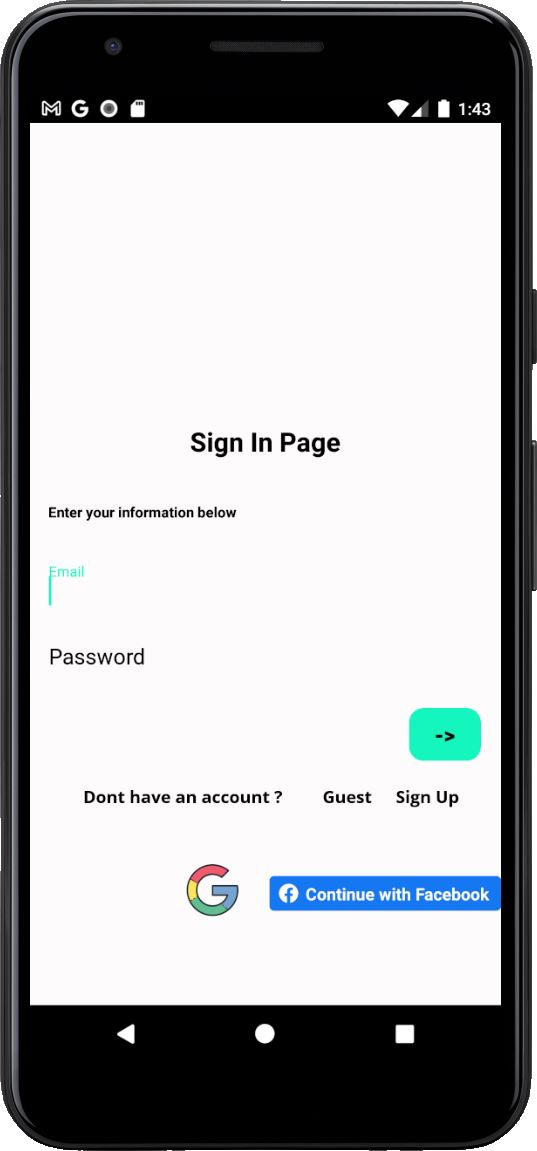
\includegraphics[width=0.35\textwidth]{final-year-project-template-master/img/FinalLoginScreen.JPG}
        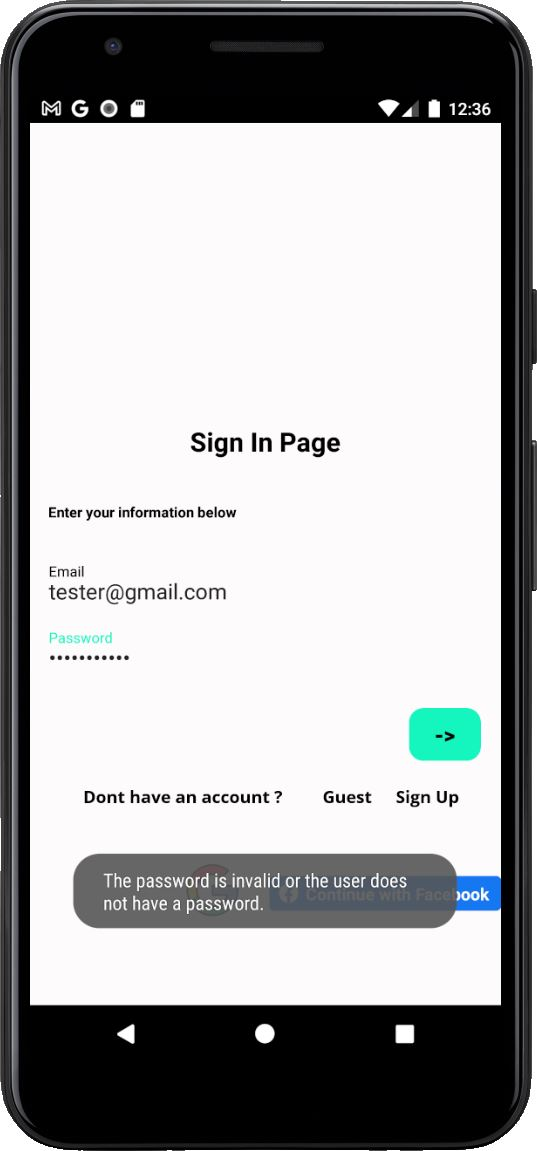
\includegraphics[width=0.35\textwidth]{final-year-project-template-master/img/incorrectPassword.JPG}

     \caption{Android Sign In screen }
\end{figure}


\subsection{Sign Up Register}
The user must register before accessing the user home screen.
I created the sign up page with a simple user interface in mind.
The sign up consists of a simple box asking for an email and password.Another option for the user is to sign up with am already existing Facebook or Google or Account.The text entered are authenticated to make sure the users details dont already exist , once successful the  user is directly displayed to the dashboard.


\begin{figure}[H]
  \centering
    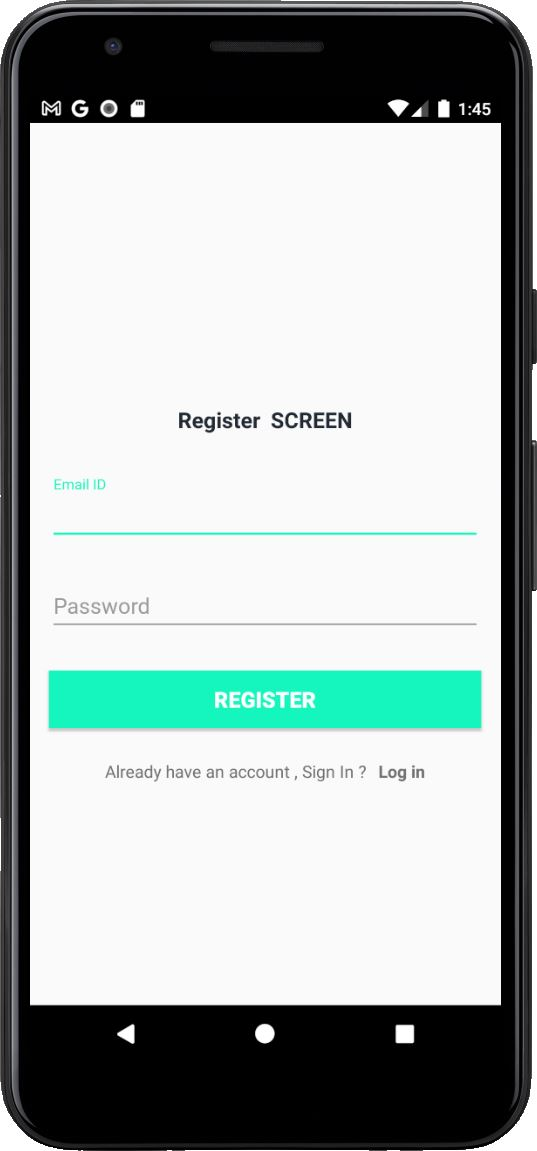
\includegraphics[width=0.35\textwidth]{final-year-project-template-master/img/finalresgisterscreen.JPG}
        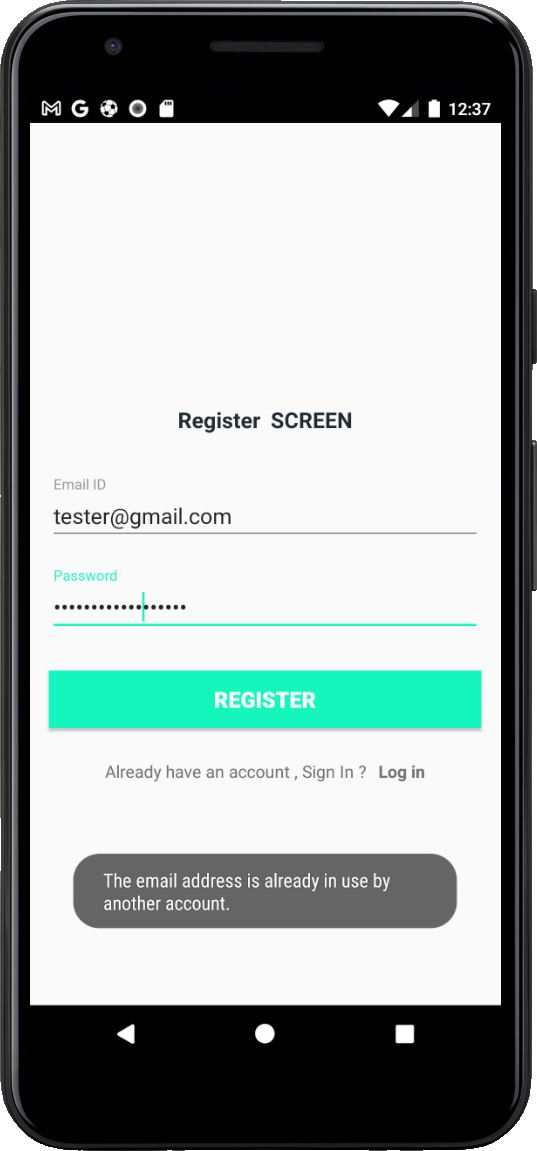
\includegraphics[width=0.35\textwidth]{final-year-project-template-master/img/alreadyexitsaccount.JPG}

     \caption{User Register on android device}
\end{figure}


The Register page uses Kotlin to make contact with the fire-base authenticator and is the user interface is created using XML.The user is displayed two text boxes on screen for their personal email and password.When the user provides an already existing email or 

\begin{lstlisting}[language=Java, caption=Facebook Login /Sign up ]
class RegisterActivity : AppCompatActivity() {
    override fun onCreate(savedInstanceState: Bundle?) {
        super.onCreate(savedInstanceState)
        setContentView(R.layout.activity_register)

        // Activity displyed in full screen
        window.decorView.systemUiVisibility = View.SYSTEM_UI_FLAG_FULLSCREEN

        // event handler for return back button
        tv_login.setOnClickListener { onBackPressed() }

        // event handler for register button
        btn_register.setOnClickListener {
            when {
                // lambda expression user email empty
                TextUtils.isEmpty(et_register_email.text.toString().trim { it <= ' ' }) -> {
                    // display message for text
                    Toast.makeText(this@RegisterActivity, "Please enter email.", Toast.LENGTH_SHORT)
                        .show()
                }
                // lambda expression user password empty
                TextUtils.isEmpty(et_register_password.text.toString().trim { it <= ' ' }) -> {
                    // display message for text in activity
                    Toast.makeText(
                        this@RegisterActivity,
                        "Please enter password.",
                        Toast.LENGTH_SHORT
                    )
                        .show()
                }
                else -> {

                    // compare and  matches the same characters
                    val email: String = et_register_email.text.toString().trim { it <= ' ' }
                    val password: String = et_register_password.text.toString().trim { it <= ' ' }

                    // Create an instance and create a register a user with email and password.
                    FirebaseAuth.getInstance()
                        .createUserWithEmailAndPassword(email, password)
                        .addOnCompleteListener(
                            OnCompleteListener<AuthResult> { task ->

                                // if the registration is successfully done
                                if (task.isSuccessful) {

                                    // Firebase registered user
                                    val firebaseUser: FirebaseUser = task.result!!.user!!

                                    // display message for text in activity
                                    Toast.makeText(
                                        this@RegisterActivity,
                                        "You are registered successfully",
                                        Toast.LENGTH_SHORT
                                    )
                                        .show()

                                    val intent =
                                        Intent(this@RegisterActivity, MainActivity::class.java)
                                    intent.flags =
                                        Intent.FLAG_ACTIVITY_NEW_TASK or
                                                Intent.FLAG_ACTIVITY_CLEAR_TASK

                                    // adds extended data to the intent.
                                    intent.putExtra("user_id", firebaseUser.uid)
                                    intent.putExtra("email_id", email)
                                    startActivity(intent)
                                    finish()
                                } else {

                                    // If the registering is not successful then show error message.
                                    Toast.makeText(
                                        this@RegisterActivity,
                                        task.exception!!.message.toString(),
                                        Toast.LENGTH_SHORT
                                    )
                                        .show()
                                }
                            }
                        )
                }
            }
        }
    }
}


\end{lstlisting}



\subsection{User Dashboard}
Once signed in the user is greeted by the dashboard activity where they can click on a series of buttons. The dashboard components are as follows

\begin{enumerate}
  \item \textbf{Quizzes}
  \item  \textbf{Calendar}
  \item \textbf{View Posts} 
  \item \textbf{Create Post}  
  \item \textbf{My Account}    
   \item \textbf{About Us}      
\end{enumerate}



  \begin{figure}[H]
  \centering
    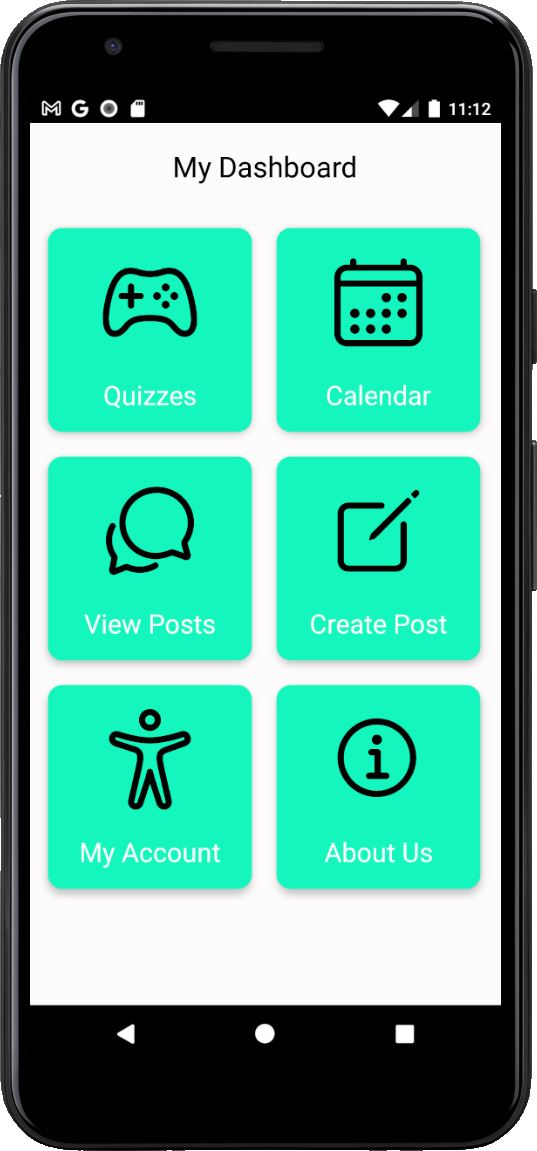
\includegraphics[width=0.35\textwidth]{final-year-project-template-master/img/fullDash.JPG}
     \caption{Android user Dashboard}
\end{figure}

As displayed in Figure 5.6 I decided on creating a simple tile styled user interface. The Dashboard is the only component in the application to use the GridLayout view.Each tile is composed of a text view , image and an ID . A unique ID allows for each of the icons to trigger a on click event to launch the component.The user navigates the application by tapping the icons on screen.


\begin{lstlisting}[language=Java, caption=Dashboard Kotlin Activity code stubs ]

class DashboardActivity : AppCompatActivity() {
    override fun onCreate(savedInstanceState: Bundle?) {
        super.onCreate(savedInstanceState)
        setContentView(R.layout.activity_dashboard)

       //Launches the Calender Activity inside of the user DashBoard view
        calenderBox_btn.setOnClickListener {

            startActivity(Intent(this@DashboardActivity, CalenderActivity::class.java))
        }
    }

\end{lstlisting}

As shown in Listing 5.8 each tile has a unique value defined in the activitydashboards.xml file,Once clicked on the startActivity() method begins the activity which is specified in the parameters.I created 6 separate buttons and with unique ids to create navigation between activities.Each tile is provided with an image and title,The images used in the application are stored in res/drawable folder. 


\subsection{Calendar Component}
A huge positive to using Kotlin is its views. I created an interactive calendar using the built-in google views. The calendar uses CRUD (Create Read Update Delete) alongside an SQ-Lite database.After researching online google provides documentation on how to add a unique calendar view\cite{calenderview}The user can create a list of reminders for whatever activities they plan. The application can be accessed offline by using the Guest option. I chose the SQ-lite database as the information is stored directly and locally onto the smart device instead of the mongodb server.


\begin{figure}[H]
  \centering
    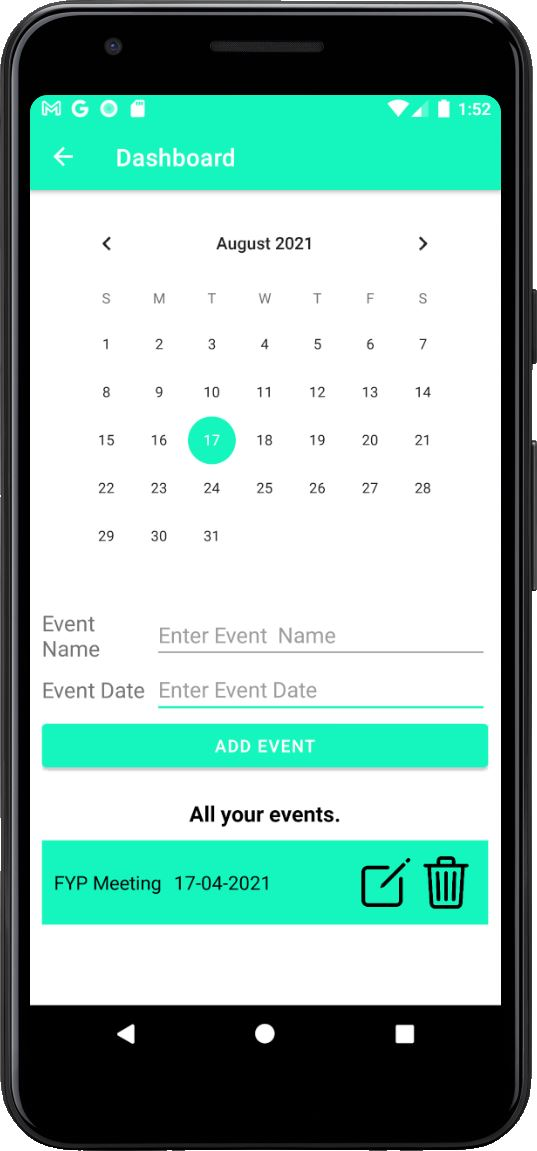
\includegraphics[width=0.35\textwidth]{final-year-project-template-master/img/AddedCalanderEvemt.JPG}
     \caption{User Calendar Screen}
\end{figure}


As shown in figure 5.7 the user is presented with  a calendar view , two edit boxes for creating an event , a create and a delete record button lastly.I created a specific activity named  CalenderActivity to update , delete , retrieve lists of events.The SQL database is the database handler class and creates the schema . It was essential to add a item adapter to convert the ArrayList of objects and view inside of my Activity.I experimented binding the calenders date selected by the user to the EventDate ID but had to settle on using the users input.






 \begin{figure}[H]
  \centering
    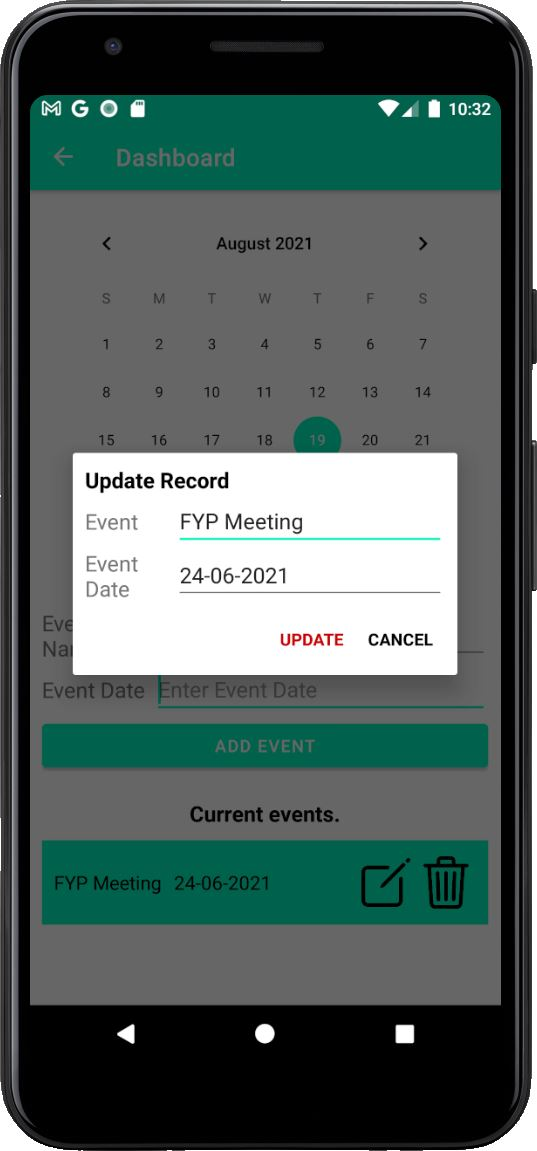
\includegraphics[width=0.35\textwidth]{final-year-project-template-master/img/updateCalenderComp.JPG}
        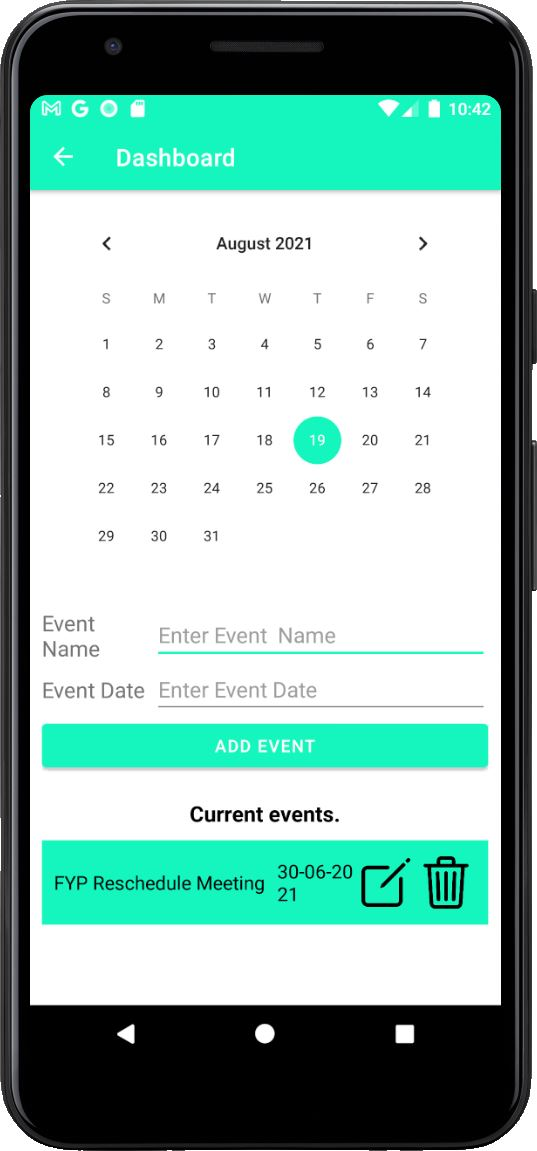
\includegraphics[width=0.35\textwidth]{final-year-project-template-master/img/suceccsfuleditcalender.JPG}

     \caption{User  Update Event Calendar Screen}
\end{figure}

The user can edit a record by pressing the edit button located at the left bottom of the screen.Once pressed the user is prompted with two text boxes to populate, once complete the user presses the update button they return to the home screen with an updated record.


\begin{lstlisting}[language=Java, caption=Update Calendar Event  ]

        val updateDialog = Dialog(this,
            R.style.Theme_Dialog
        )
        updateDialog.setCancelable(false)

        updateDialog.setContentView(R.layout.dialog_update)

        updateDialog.etUpdateName.setText(calenderModelClass.name)
        updateDialog.etUpdateDATEId.setText(calenderModelClass.date)

        updateDialog.tvUpdate.setOnClickListener(View.OnClickListener {

\end{lstlisting}



 \begin{figure}[H]
  \centering
  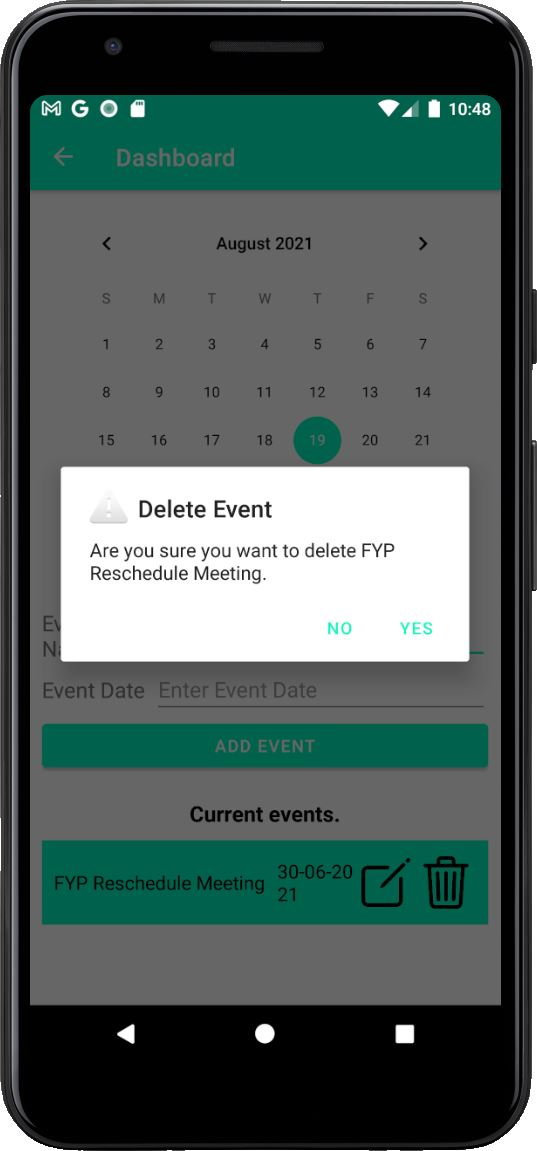
\includegraphics[width=0.35\textwidth]{final-year-project-template-master/img/deleteEvemtSuccesss.JPG}
    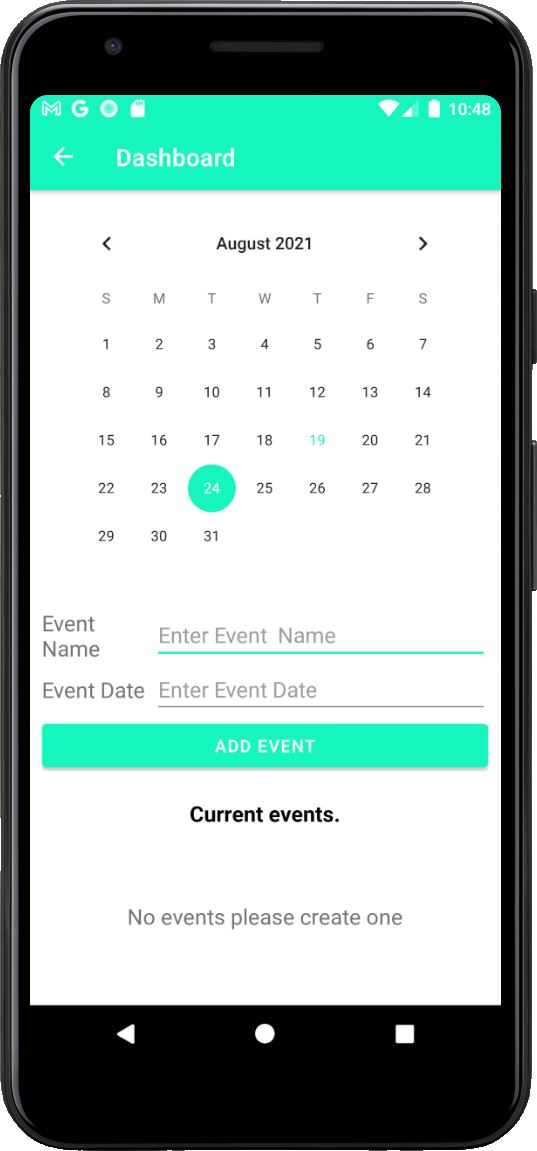
\includegraphics[width=0.35\textwidth]{final-year-project-template-master/img/deletedeventcaledner.JPG}

     \caption{User  Delete  Event Calendar Screen}
\end{figure}

\begin{lstlisting}[language=Java, caption=Update Calendar Event  ]
     //creating the instance of DatabaseHandler class
            val databaseHandler: DatabaseHandler =
                DatabaseHandler(this)
            //calling the deleteUser method of DatabaseHandler class to delete record


            val status = databaseHandler.deleteEvent(
                calenderModelClass(
                    calenderModelClass.id,
                    "",
                    ""
                )
            )
            if (status > -1) {
                // event message displayed to user when successful
                Toast.makeText(
                    applicationContext,
                    "Event deleted successfully.",
                    Toast.LENGTH_LONG
                ).show()
                // displays list in a view in application
                setupListofDataIntoRecyclerView()
            }

            dialogInterface.dismiss() // Dialog will be dismissed
\end{lstlisting}

\subsection{User Account Component}

After the user has signed up they can view their profile details such as their name, profile picture, and email address. The component displays directly the details entered from the register component. The details of all users can be viewed from the fire-base google console.


\begin{figure}[H]
  \centering
  
    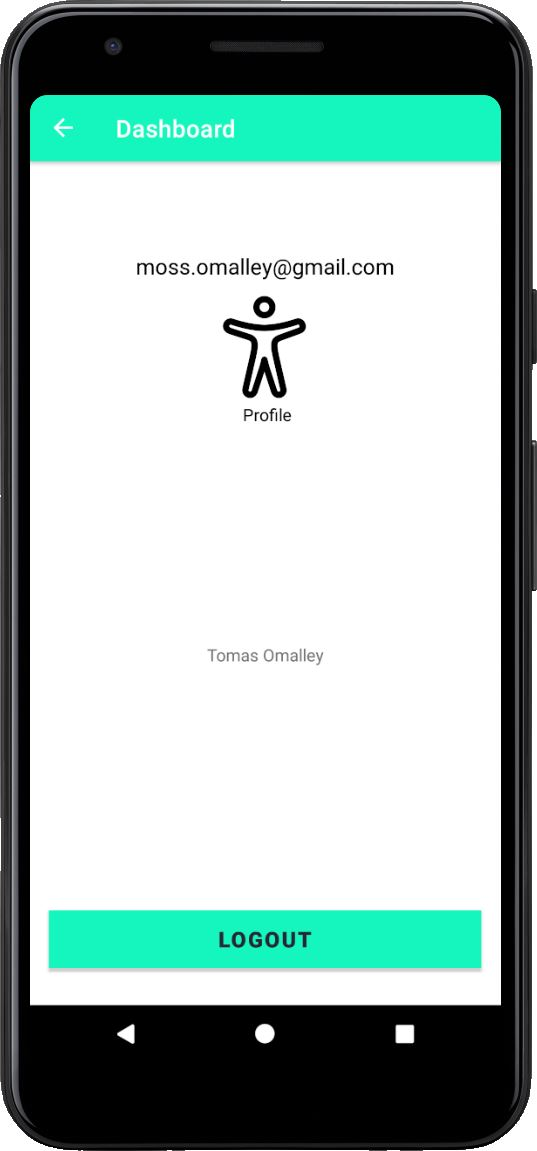
\includegraphics[width=0.35\textwidth]{final-year-project-template-master/img/userprofilefull.JPG}

     \caption{Android User Profile}
\end{figure}






\begin{lstlisting}[language=Java, caption=Dashboard Kotlin User Profile code stubs ]

 // instantiate authenticator client
        mAuth = FirebaseAuth.getInstance()
        val currentuser = mAuth.currentUser

        // Display the current details for sign in user to screen
        id_txt.text = currentuser?.uid
        name_txt.text = currentuser?.displayName
        email_txt.text = currentuser?.email

\end{lstlisting}

The code stubs in Listing 5.9 display the Kotlin  codebase for the user profile.The userProfileActivity creates a new instance of the firebase client , once connected the unique identifiers are data binded using the current details in the firebase db, .text was used to convert and map the string to the Text-view  defined in activity user profile.xml




\subsection{About App Component   }


In the about app page , I explain the object of the application and the version type.While researching online I noticed a  prominent trend of the addition of an about page.The component will be of use for bugging if the user has issues with the application , The user can compare their app version in the android store and choose to update to help resolve any future issues.The about page uses a text view and an image view to retrieve my application logo and the text.The user can click on the GitHub text to be sent to my GitHub Repository to learn more about future updates.

 \begin{figure}[H]
  \centering
    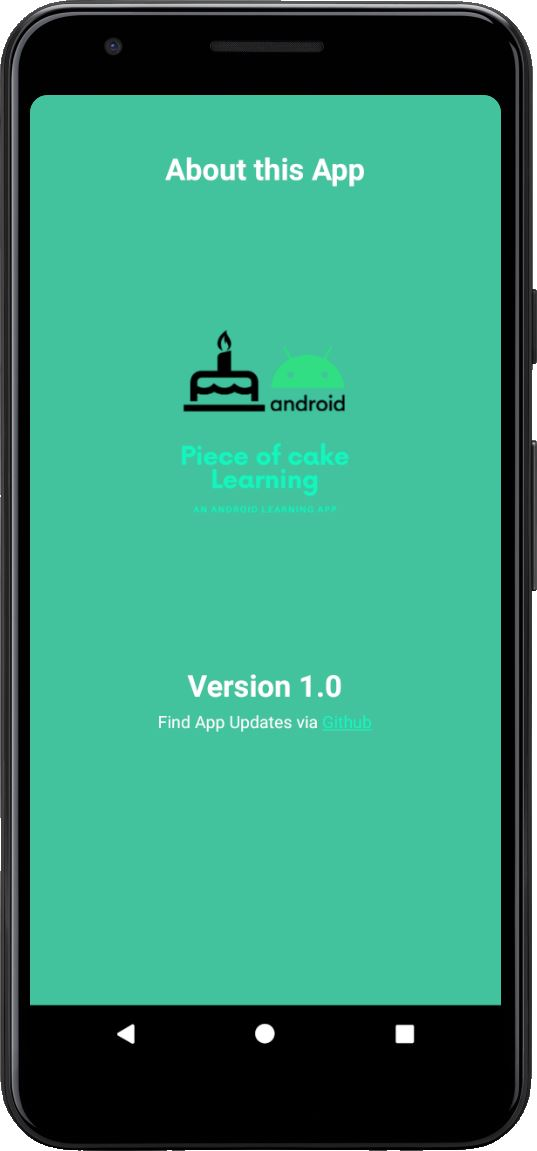
\includegraphics[width=0.35\textwidth]{final-year-project-template-master/img/finalaboutpage.JPG}
     \caption{About App Screen}
\end{figure}



\begin{lstlisting}[language=Java, caption=Dashboard  About Us Kotlin code stubs ]
// Call Hyper Link
setupHyperlink()

    }
    // function declaration bind view clickable link
        fun setupHyperlink() {
            val linkTextView = findViewById<TextView>(R.id.githublinktv)
            linkTextView.setMovementMethod(LinkMovementMethod.getInstance());
        }
\end{lstlisting}

The codestubs in listing 5.10 provide the functionality for the about us Activity.The class consists of a function that creates  a clickable link that transfers the user to their browser to view my github page.I created a specific string in the Strings.xml file to be called by the activity displayed in listing 5.11



\begin{lstlisting}[language=XML, caption=Dashboard  About Us Kotlin code stubs ]

    <a href= "https://github.com/OmalleyFinalYearAppliedProject/FinalYearAppliedProjectGMIT">Find Updates via Github</a>
\end{lstlisting}

The AboutUs page renders this link uses the LinkMovementMethod() to navigate the user to the browser.



\subsection{Posts Component}
The Post component acts an area of the application where the user can read posts created with queries ranging from Hardware for sale or Computer  grinds available.The screen consists of a listview which loops through an array of objects hosted in my Node JS server.Each object is formatted into the list and the user can read and contact for more information

 \begin{figure}[H]
  \centering
    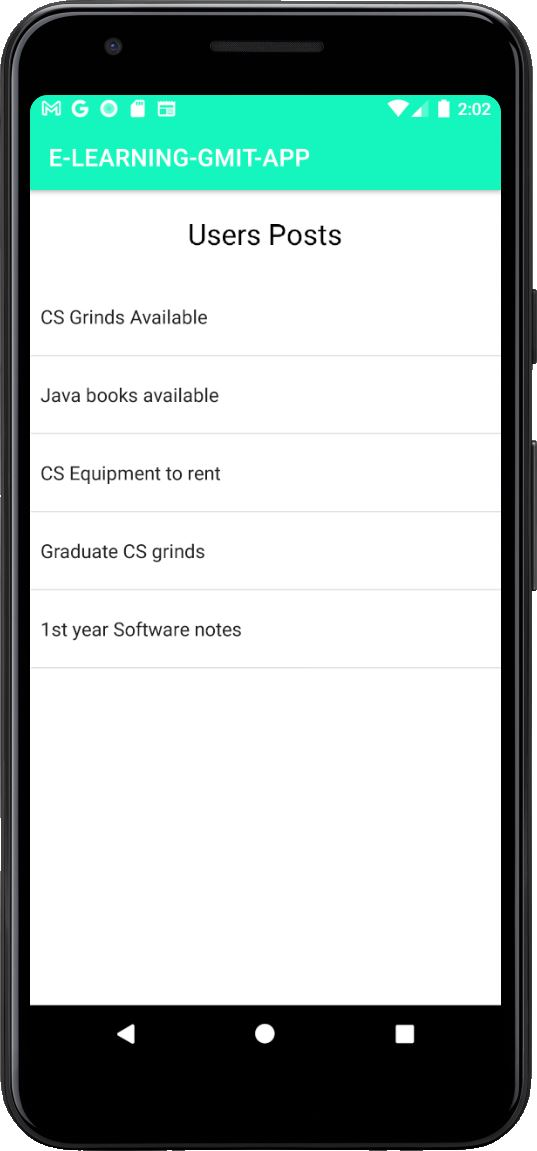
\includegraphics[width=0.35\textwidth]{final-year-project-template-master/img/postscomponent.JPG}
     \caption{Posts Component}
\end{figure}


\begin{lstlisting}[language=Java, caption=Posts Interface HTTP GET ]

 // OKHTTP NETWORK GET REQUEST FOR QUESTIONS API
    @get:GET("posts")
    // CREATE STORE POSTS INTO A LIST
    val forumposts : Call<List<PostModel?>?>

    // OBJ HOLDS URL TO SERVER
    companion object {
        const val BASE_URL = "https://quiz-node-js-backend.herokuapp.com/"
    }
\end{lstlisting}
I created an interface as shown in listing 5.12 to allow for the  HTTP method GET to allow for the retrieval of my JSON formatted records in my Model Post class displayed in listing 5.13

\begin{lstlisting}[language=Java, caption= PostModel Model class ]

class PostModel {

    // Post MODEL HOLDING INSTANCE VARIABLES
    var userId = 0
    var id = 0
    var title: String? = null
    var active: String? = null
    var student: String? = null
    var teacher: String? = null
}
\end{lstlisting}


After the model and the GET request is created the PostFeed creates an instance of the Retrofit Client using the stored array of objects Type post and binds to the listview created in activitypostfeed.xml as shown below in listing in Listing 5.14
\begin{lstlisting}[language=Java, caption= Render Arraylist  to view ]

   var postList: List<PostModel>? = response.body() as List<PostModel>
                var post = arrayOfNulls<String>(postList!!.size)

                // loop over posts
                for (i in postList!!.indices)
                    post[i] = postList!![i]!!.title


                var adapter = ArrayAdapter<String>(
                    applicationContext,
                    android.R.layout.simple_dropdown_item_1line,
                    post
                )
                listview.adapter = adapter
\end{lstlisting}
\subsection{Create Post Component}
The Post component acts an area of the application where the user can read posts created with queries ranging from Hardware for sale or Computer  grinds available.The create post consists of 4 parameters the user must populate before pushing a post to the view posts component.The posts are pulled from my Node JS back-end server using the MVM design pattern and the retrofit a rest client library\cite{retrofit}.

 \begin{figure}[H]
  \centering
    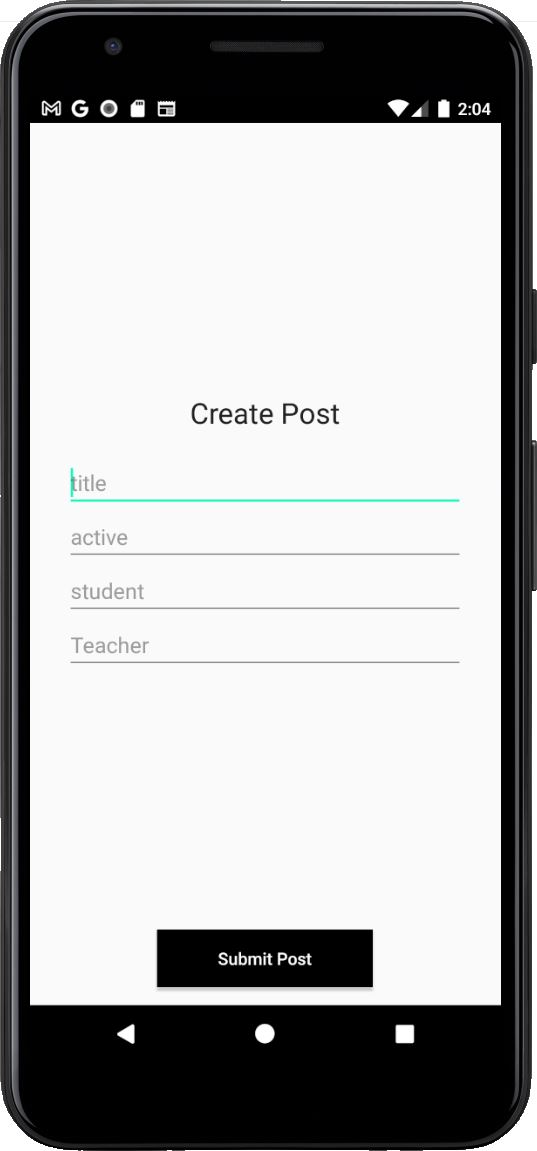
\includegraphics[width=0.35\textwidth]{final-year-project-template-master/img/Createpostcomponent.JPG}
     \caption{Create Posts Component}
\end{figure}


\begin{lstlisting}[language=Java, caption= user input from xml view ]

        buttonCreatePost.setOnClickListener {

            val title = editPostTitle.text.toString().trim()
            val active = editPostActive.text.toString().trim()
            val student = editPostStudent.text.toString().trim()
            val teacher = editPostTeacher.text.toString().trim()
\end{lstlisting}

The codestubs displayed in Listing 5.15 display the code to create a post the user must enter 4 parameters , once converted to text they are pushed using a Post request using the Retrofit Client. 

\begin{lstlisting}[language=Java, caption=Create Post Model for HTTP Post Retrofit request ]

  // OBJ HOLDS URL TO SERVER
    companion object {
        const val BASE_URL = "https://quiz-node-js-backend.herokuapp.com/"
    }
    // Post request create posts
    @FormUrlEncoded
  @POST("createpost")
    fun createPost(
        @Field( "title") title:String,
        @Field( "active") active:String,
        @Field( "student") student:String,
        @Field( "teacher") teacher:String

\end{lstlisting}

Listing  5.16 displays the parameters needed from the user to successfully create a POST request to push user input the Backend server.

\subsection{Quiz Component}
The Quiz component is the brain of the application. The user is greeted with a welcome page where the user must enter their name before continuing.The Quiz component is the centre point of the application.Once successfully entering their name they can start a quiz. The structure of the quizzes are in multiple choice.When correct the user receives a green tick and when incorrect receives a red tick.








 \begin{figure}[H]
  \centering
    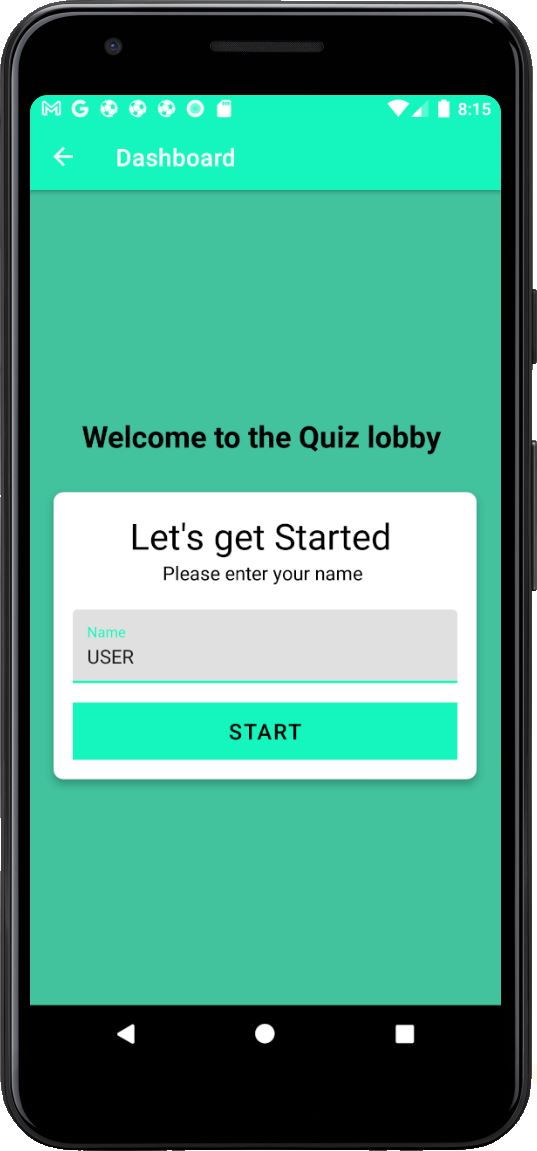
\includegraphics[width=0.35\textwidth]{final-year-project-template-master/img/quizlobby.JPG}
     \caption{Quiz user welcome Lobby}
\end{figure}
As displayed in fig5.15 the user is greeted in the question lobby.I implemented an edit text box to allow for user input textbox while before starting the game.The user cannot proceed until they enter a string into the edit-text box.Once the user has pressed the start button they are sent to the quiz screen.


\begin{lstlisting}[language=Java, caption=Question Lobby CodeSnippets  ]

  btn_start.setOnClickListener {

            if (et_name.text.toString().isEmpty()) {

                // Display text to user
                Toast.makeText(
                    this,
                    "Please enter your name ", Toast.LENGTH_SHORT
                ).show()
            } else {

                // Start activity once entered
                val intentQs = Intent(this, QuizQuestionsActivity::class.java)
                intent.putExtra(Constants.USER_NAME,et_name.text.toString())
                startActivity(intentQs)
                // end
                finish()

            }

\end{lstlisting}


 \begin{figure}[H]
  \centering
    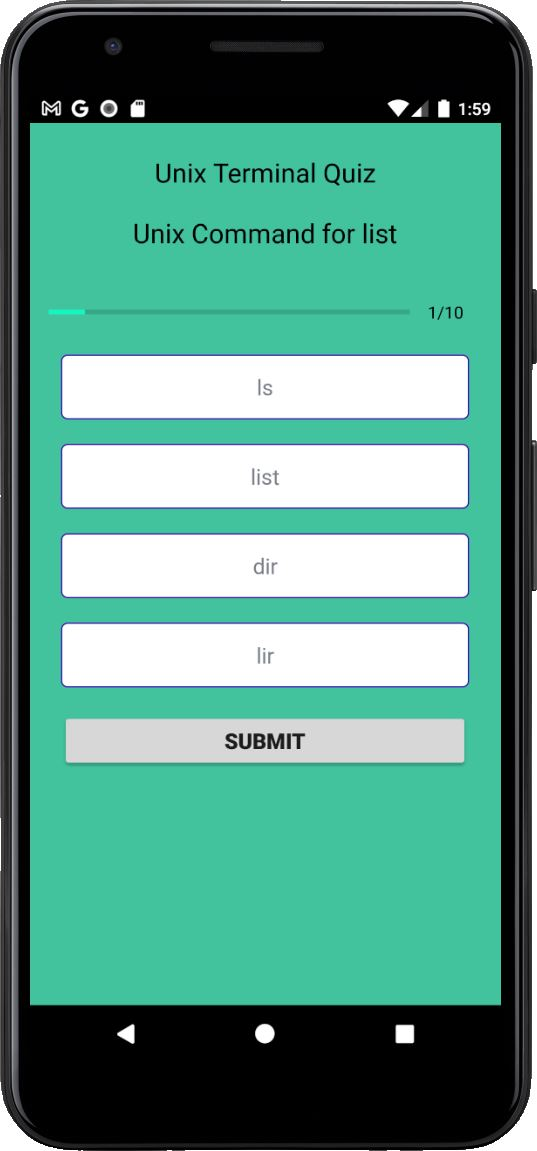
\includegraphics[width=0.35\textwidth]{final-year-project-template-master/img/QuizScreenFinal.JPG}
     \caption{user Sample Quiz}
\end{figure}

The user is displayed the quiz name , the question a progress bar followed by the multiple choice answers.The user clicks on the answer they believe is correct.Figure 5.16 displays the user interface of the quiz.


\begin{lstlisting}[language=Java, caption=Onclick method for  ]
   //Map constant text to on screen button
        tv_question.text = question!!.question
        tv_option_one.text = question.optionOne
        tv_option_two.text = question.optionTwo
        tv_option_three.text = question.optionThree
        tv_option_four.text = question.optionFour


// On click handler  for user selection in MCQ
 when (v?.id) {
            R.id.tv_option_one -> {

                selectedOptionView(tv_option_one, 1)
            }
            R.id.tv_option_two -> {

                selectedOptionView(tv_option_two, 2)
            }
            R.id.tv_option_three -> {

                selectedOptionView(tv_option_three, 3)
            }
            R.id.tv_option_four -> {

                selectedOptionView(tv_option_four, 4)
            }
            
            
\end{lstlisting}

 \begin{figure}[H]
  \centering
    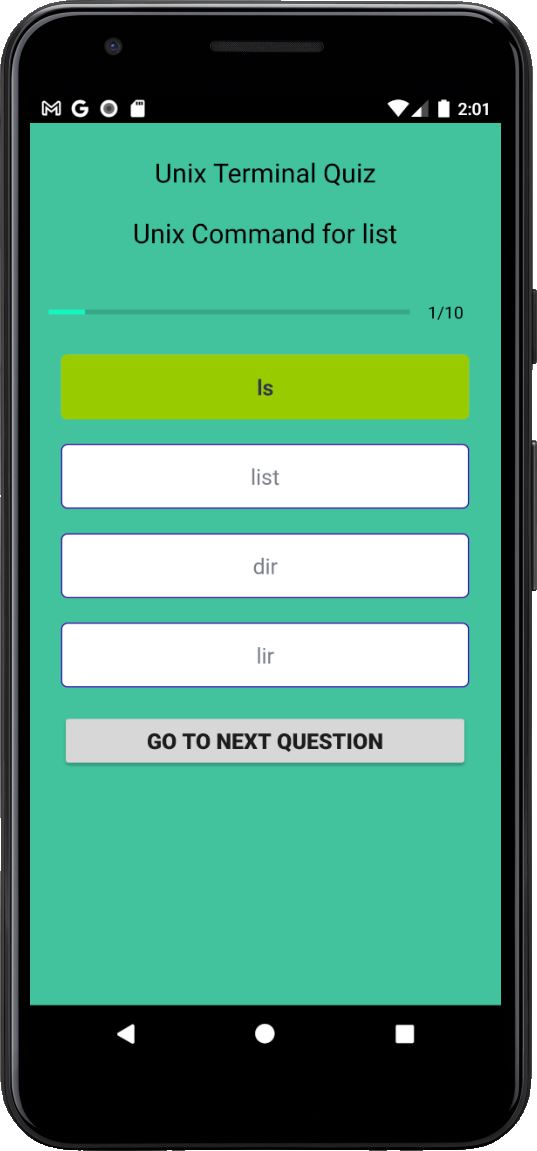
\includegraphics[width=0.35\textwidth]{final-year-project-template-master/img/correctAnswerHighlight.JPG}
     \caption{user Unix Quiz}
\end{figure}

Once the user selects a choice the border becomes highlighted to ensure the user is happy with their choice , when correct the choice will display green and the button will update asking the user to go to the next question as displayed in Fig5.17.

 

 \begin{figure}[H]
  \centering
    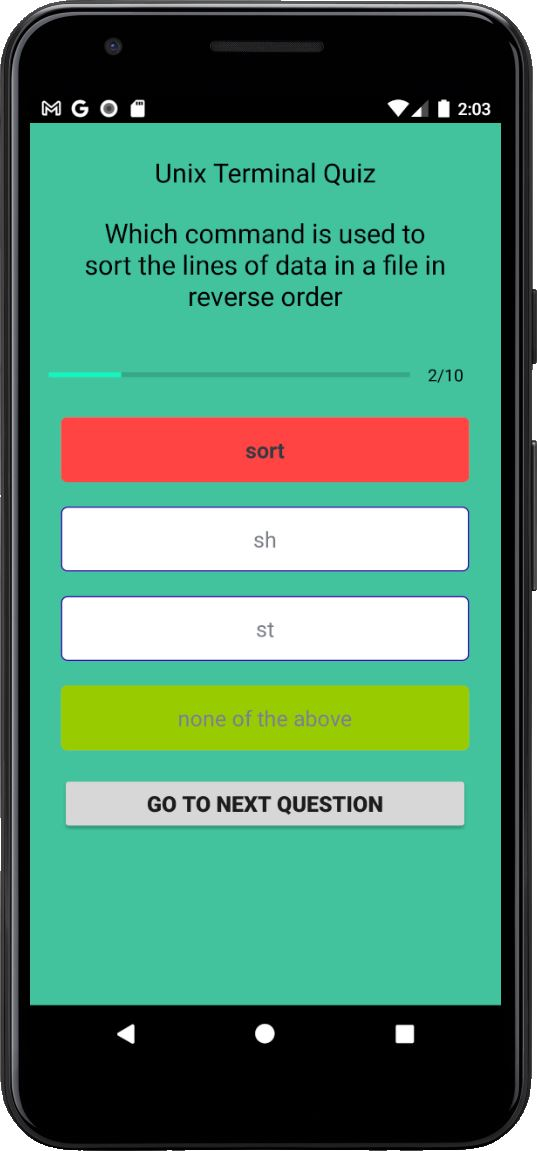
\includegraphics[width=0.35\textwidth]{final-year-project-template-master/img/IncorrectAnsQuestions.JPG}
     \caption{user Incorrect Answer}
\end{figure}
Once the users clicks one of the four buttons if the users choice is incorrect the correct answer will be displayed in green and when incorrect it will display as red.



\begin{lstlisting}[language=Java, caption= Incorrect Answer border ]

 if (question!!.correctAnswer != mSelectedOptionPosition) {

    answerView(mSelectedOptionPosition,
        R.drawable.wrong_option_border_bg)
                    
    }else
    {
      mCorrectAnswers++
     }

     answerView(question.correctAnswer,
    R.drawable.correct_option_border_bg
    )


\end{lstlisting}

The codestubs in Listing 5.17 display the correct and wrong border for the user using a special view named the answerView.After displaying the view the users score is added with a counter.

 \begin{figure}[H]
  \centering
    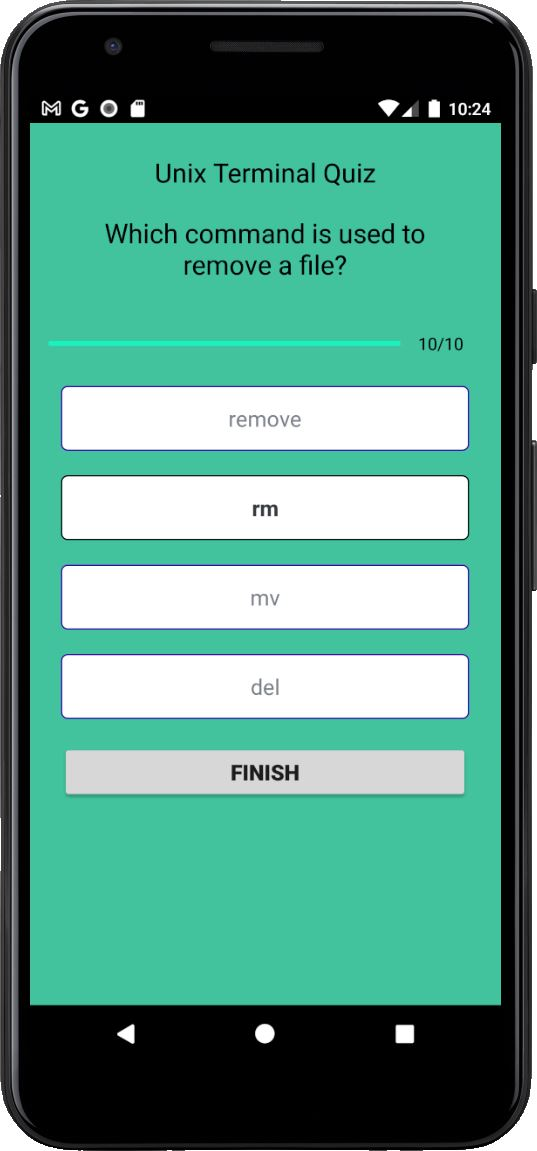
\includegraphics[width=0.35\textwidth]{final-year-project-template-master/img/finalqpage.JPG}
     \caption{user Incorrect Answer}
\end{figure}
Once the user completes all the questions the submit button event handles and displays a Finish button.Each correct answer is stored in a counter and is saved using a coroutine method.




 \begin{figure}[H]
  \centering
    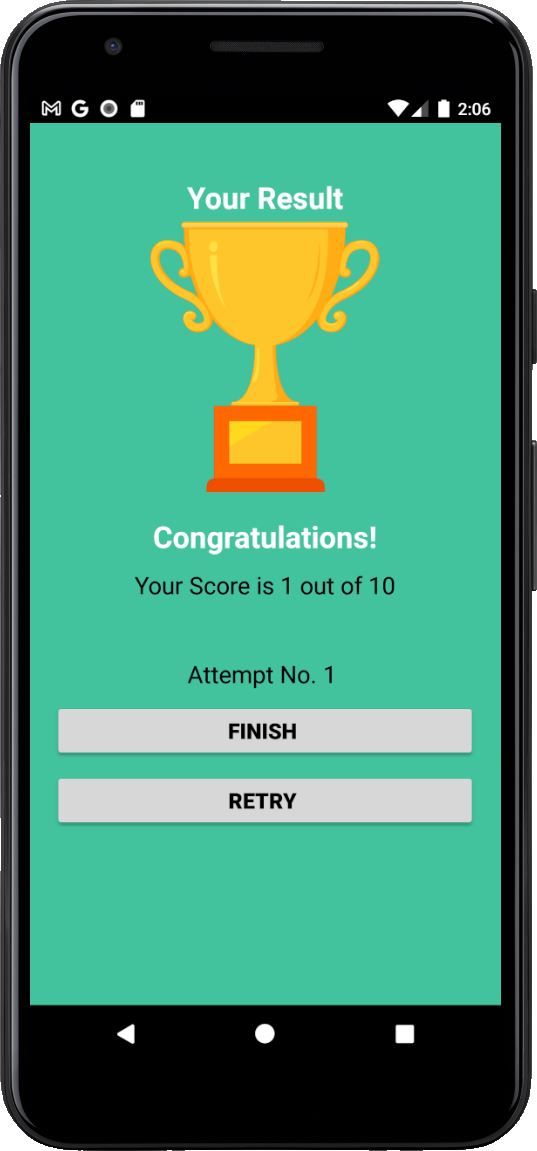
\includegraphics[width=0.35\textwidth]{final-year-project-template-master/img/userresultscreen.JPG}
     \caption{user Quiz Results}
\end{figure}
After completing all ten questions the user is displayed the result page as shown in Fig5.20.The screen displays the users result alongside two separate buttons to retry or to finish and return to the dashboard.




\begin{lstlisting}[language=Java, caption= Incorrect Answer border ]

        val totalQs  = intent.getIntExtra(Constants.TOTAL_QUESTIONS,0)
        val correctAns   = intent.getIntExtra(Constants.Correct_Ans,0)
        val noOfQuizzesTaken   = intent.getIntExtra(Constants.Correct_Ans,0)

        // bind user score from constants
        tv_score.text = "Your Score is $correctAns out of $totalQs"
        tv_attempt.text = "Attempt No. $noOfQuizzesTaken "
\end{lstlisting}


\subsection{Data Management}
Consumers are more than ever more aware/conscious of why and where their personal data is stored. As of 2021, the worldwide information security market is forecast to reach 170.35 billion dollars. I settled on strong a strong back-end with Google's strong fire-base back-end to give users the strongest protection.

\subsection{Data Gathering}


In this section, I will discuss the ways I gathered data for my quiz application. To display data I used an array of dependencies for allowing my application to be network configured and end to end. 

\begin{itemize}
\item    \textbf{OKHTTP}
 is a popular network access dependency used in android applications for the retrieval of  data\cite{okhttp}.It is an open source software suit that supports all requests to a socket network.The OKHTTP provides a massive roll in retrieving the data stored in my server.


\begin{lstlisting}[language=Java, caption= OKHTTP GET REQUEST]
   @get:GET("questions")
      val posts : Call<List<FeedModel?>?>

        companion object {
            const val BASE_URL = "https://cloud-backend-js.herokuapp.com"    

\end{lstlisting}




When creating the application I aimed to host the questions online using mongodb.After issues with speed I decided to store the questions locally and display using the MVVM application model.

\begin{lstlisting}[language=Java, caption= Question Model]

data class Question(

    // DEF OF QUESTION LIST STRUCTURE
    val id: Int,
    val question: String,
    val optionOne: String,
    val optionTwo: String,
    val optionThree: String,
    val optionFour: String,
    val correctAnswer: Int

    )
    \end{lstlisting}



\end{itemize}


\begin{lstlisting}[language=Java, caption= Hard  Coded Questions]


// function with a list of questions hard coded and displayed in quiz questions activity
    fun getQuestions(): ArrayList<Question>
    {
        val questionsList = ArrayList<Question>()
        val que1 = Question(
            1, "Unix Command for list",
             "ls"
            , "list", "dir", "lir", 1
        )
\end{lstlisting}

As shown in listing 5.14 the structure of the hard coded questions.I experimented with saving the constants in my mongodb schema but with no success had to create the answers as constants



\subsection{Application Components  }
In this section, I will break down into the pieces of the different pieces of my application.

\subsection{Application   Management }

JSON is an open standard file format, and data interchange format, that uses human-readable text to store and transmit data objects consisting of attribute-value pairs and array data types. I decided to parse the JSON stored on my ruby on rails application deployed to Heroku.


\begin{verbatim}


JSON API on Node JS 
[
    {
        "_id":"6078c7659e1812689efab089",
        "description":"Unix command to list all files on system ",
        "alternatives":[
            {
                "0":"l",
                "1":"s",
                "isCorrect":false
            },
            {
                "0":"l",
                "1":"i",
                "2":"s",
                "3":"t",
                "isCorrect":false
            },
            {
                "0":"l",
                "1":"s",
                "2":"t",
                "isCorrect":false
            },
            {
                "0":"d",
                "1":"i",
                "2":"r",
                "isCorrect":false
            }
        ]
        
 Above is the formatted data for the questions component.

\end{verbatim}

The API  relies on the  technologies of Javascript  , Node JS , Mongo .I created  a series of APIs to allow bridge point my mobile application  and the back-end.

\begin{lstlisting}[language=Java, caption=API URL Endpoints]
     // Server Home
     https://quiz-node-js-backend.herokuapp.com/
     
     // Questions
     https://quiz-node-js-backend.herokuapp.com/Questions
     
     // Posts Forum 
     https://quiz-node-js-backend.herokuapp.com/posts
     
     // Quizzes 
     https://quiz-node-js-backend.herokuapp.com/Quizzes
\end{lstlisting}







\subsection{Backend Components }
In this section, I will evaluate the components of my back-end design.



\begin{itemize}
\item\textbf{Server} 

\begin{itemize}
     \item\textbf{Server.js:} The server runs automatically and it is currently deployed to the Heroku cloud.



\begin{lstlisting}[language=Java, caption= Server.js Code Stubs ]
const express = require('express')
const app = express() // declare express
const mongoose = require('mongoose') // use mongoose 
require('dotenv').config() // include config file
const routes = require('./routes') // includes the routes.js file
const cors = require('cors') // includes cors module

app.use(cors()) //  express  using CORS
app.use(express.json()) // using json 
app.use(routes) // server to use the routes in routes.js

// mongo database 
mongoose.connect(process.env.DATABASE_URL, { useNewUrlParser: true, useUnifiedTopology: true })
const db = mongoose.connection

// error catch
db.on('error', (error) => console.error(error))
db.once('open', () => console.log('database connected'))


// app listen on port 3333
app.listen(process.env.PORT, () => {
    console.log("The API is running...")
})

\end{lstlisting}

   \end{itemize}

\item\textbf{Data Models} 

 \begin{itemize}
 
 \item\textbf{Question.js :}
 
 For the users' questions, I created a model which is stored in MongoDB atlas
 

 
 \begin{lstlisting}[language=Java, caption= Question.js Code Stubs ]

 
 const mongoose = require('mongoose')

const QuestionSchema = new mongoose.Schema({
    description: String,
    alternatives: [
        {
            text: {
                type: String,
                required: true
            },
            isCorrect: {
                type: Boolean,
                required: true,
                default: false
            }
        }
    ]
})

module.exports = mongoose.model('Question', QuestionSchema)
 
 \end{lstlisting}

 

  \item\textbf{Post.js  :}
  
  
   \begin{lstlisting}[language=Java, caption= Post Schema and Get Post Methods ]
   
   const mongoose = require('mongoose')


// Post schema for db
const PostSchema = new mongoose.Schema({
    title : String,
    active : String,
    student : String,
    teacher : String
})

// get all posts 
router.get('/posts', async (req, res) => {
    try {
        const posts = await Post.find()
        return res.status(200).json(posts)
    } catch (error) {
        return res.status(500).json({"error":error})
    }
})



module.exports = mongoose.model('Post', PostSchema)



// create a post
router.post('/createpost', async (req, res) => {
    try {
        const { title } = req.body
        const { active } = req.body        
        const { student } = req.body
        const { teacher } = req.body



        const post = await Post.create({
            title,
            active,
            student,
            teacher

        })

        return res.status(201).json(post)
    } catch (error) {
        return res.status(500).json({"error":error})
    }
})


 \end{lstlisting}


   \end{itemize}
   
  
\end{itemize}


\chapter{System Evaluation}

\subsection{Testing Tools}

   Testing plays an important  role in software applications.Four testing tools were used in my project and  are as followed :
    
    
\subsection{Unit Tests}
Here are some unit tests I carried out on my application.
\textbf{User Log In Functionality} 
 
  \begin{figure}[H]

\begin{itemize}

\begin{tabular}{ |p{3.5cm}||p{3.5cm}|p{3.5cm}|  }
 \hline
 \multicolumn{3}{|c|}{Test Expect Input/Output.  Pass or Fail } \\
 \hline
 User Log In & Credentials Correct  & Pass\\
 \hline
 User Log Out & Credentials Correct  & Pass\\
 \hline
 Social Media authentication & Credentials Correct  & Pass\\
 \hline
\end{tabular}


\end{itemize}
 \caption{User Log In / Out  unit test }
\end{figure}

 \begin{figure}[H]

\begin{itemize}
\item    \textbf{User Sign  Up  Functionality}  

\begin{tabular}{ |p{3.5cm}||p{3.5cm}|p{3.5cm}|  }
 \hline
 \multicolumn{3}{|c|}{Test Expect Input/Output.  Pass or Fail } \\
 \hline
 User Enters Sign-Up Details  & Validation  & Pass\\
 \hline
 User Enters existing Credentials  & Validation provides error  & Pass\\

 \hline

 Social Media authentication & Credentials Correct  & Pass\\

 \hline
\end{tabular}


\end{itemize}

 \caption{User Sign  Up unit test }

\end{figure}





 \begin{figure}[H]

\begin{itemize}
\item    \textbf{Add Event Calendar Feature}  

\begin{tabular}{ |p{3.5cm}||p{3.5cm}|p{3.5cm}|  }
 \hline
 \multicolumn{3}{|c|}{Test Expect Input/Output.  Pass or Fail } \\
 \hline
 User Enters Event name and Date  & Insert Record  & Pass\\
 \hline


\end{tabular}


\end{itemize}
     \caption{Add calendar unit test}

\end{figure}


 \begin{figure}[H]

\begin{itemize}
\item    \textbf{Add Event calendar Feature}  

\begin{tabular}{ |p{3.5cm}||p{3.5cm}|p{3.5cm}|  }
 \hline
 \multicolumn{3}{|c|}{Test Expect Input/Output.  Pass or Fail } \\
 \hline
 User Enters Event name and Date  & Insert Record  & Pass\\
 \hline
\end{tabular}

\end{itemize}

     \caption{Add Event Calendar unit test }

\end{figure}

 \begin{figure}[H]

\begin{itemize}
\item    \textbf{Delete Event Calendar Feature}  

\begin{tabular}{ |p{3.5cm}||p{3.5cm}|p{3.5cm}|  }
 \hline
 \multicolumn{3}{|c|}{Test Expect Input/Output.  Pass or Fail } \\
 \hline
 User selects Event and clicks remove  & Delete  Record  & Pass\\
 \hline
\end{tabular}
\end{itemize}
\caption{Delete Event Calendar unit test}
\end{figure}


\begin{figure}[H]
\begin{itemize}
\item    \textbf{Quiz Lobby Feature}  

\begin{tabular}{ |p{3.5cm}||p{3.5cm}|p{3.5cm}|  }
 \hline
 \multicolumn{3}{|c|}{Test Expect Input/Output.  Pass or Fail } \\
 \hline
 User Clicks Quiz   & Opens Quiz lobby Component   & Pass\\
 \hline
\end{tabular}

\end{itemize}. 

\caption{Quiz Lobby unit test}

\end{figure}


    
    
    
\subsection{Postman API testing}
 http testing  : Postman was an  effective  tool for testing my applications network implementation.I used the tool when testing  an API (Application Programming Interface)  for my JSON MongoDB database.Postman is a free open-source  tool for testing end points for APIs.
 I tested my questions on NodeJS by creating GET and POST conditions to my Mongo Database.
 
 
  \begin{figure}[H]
  \centering
    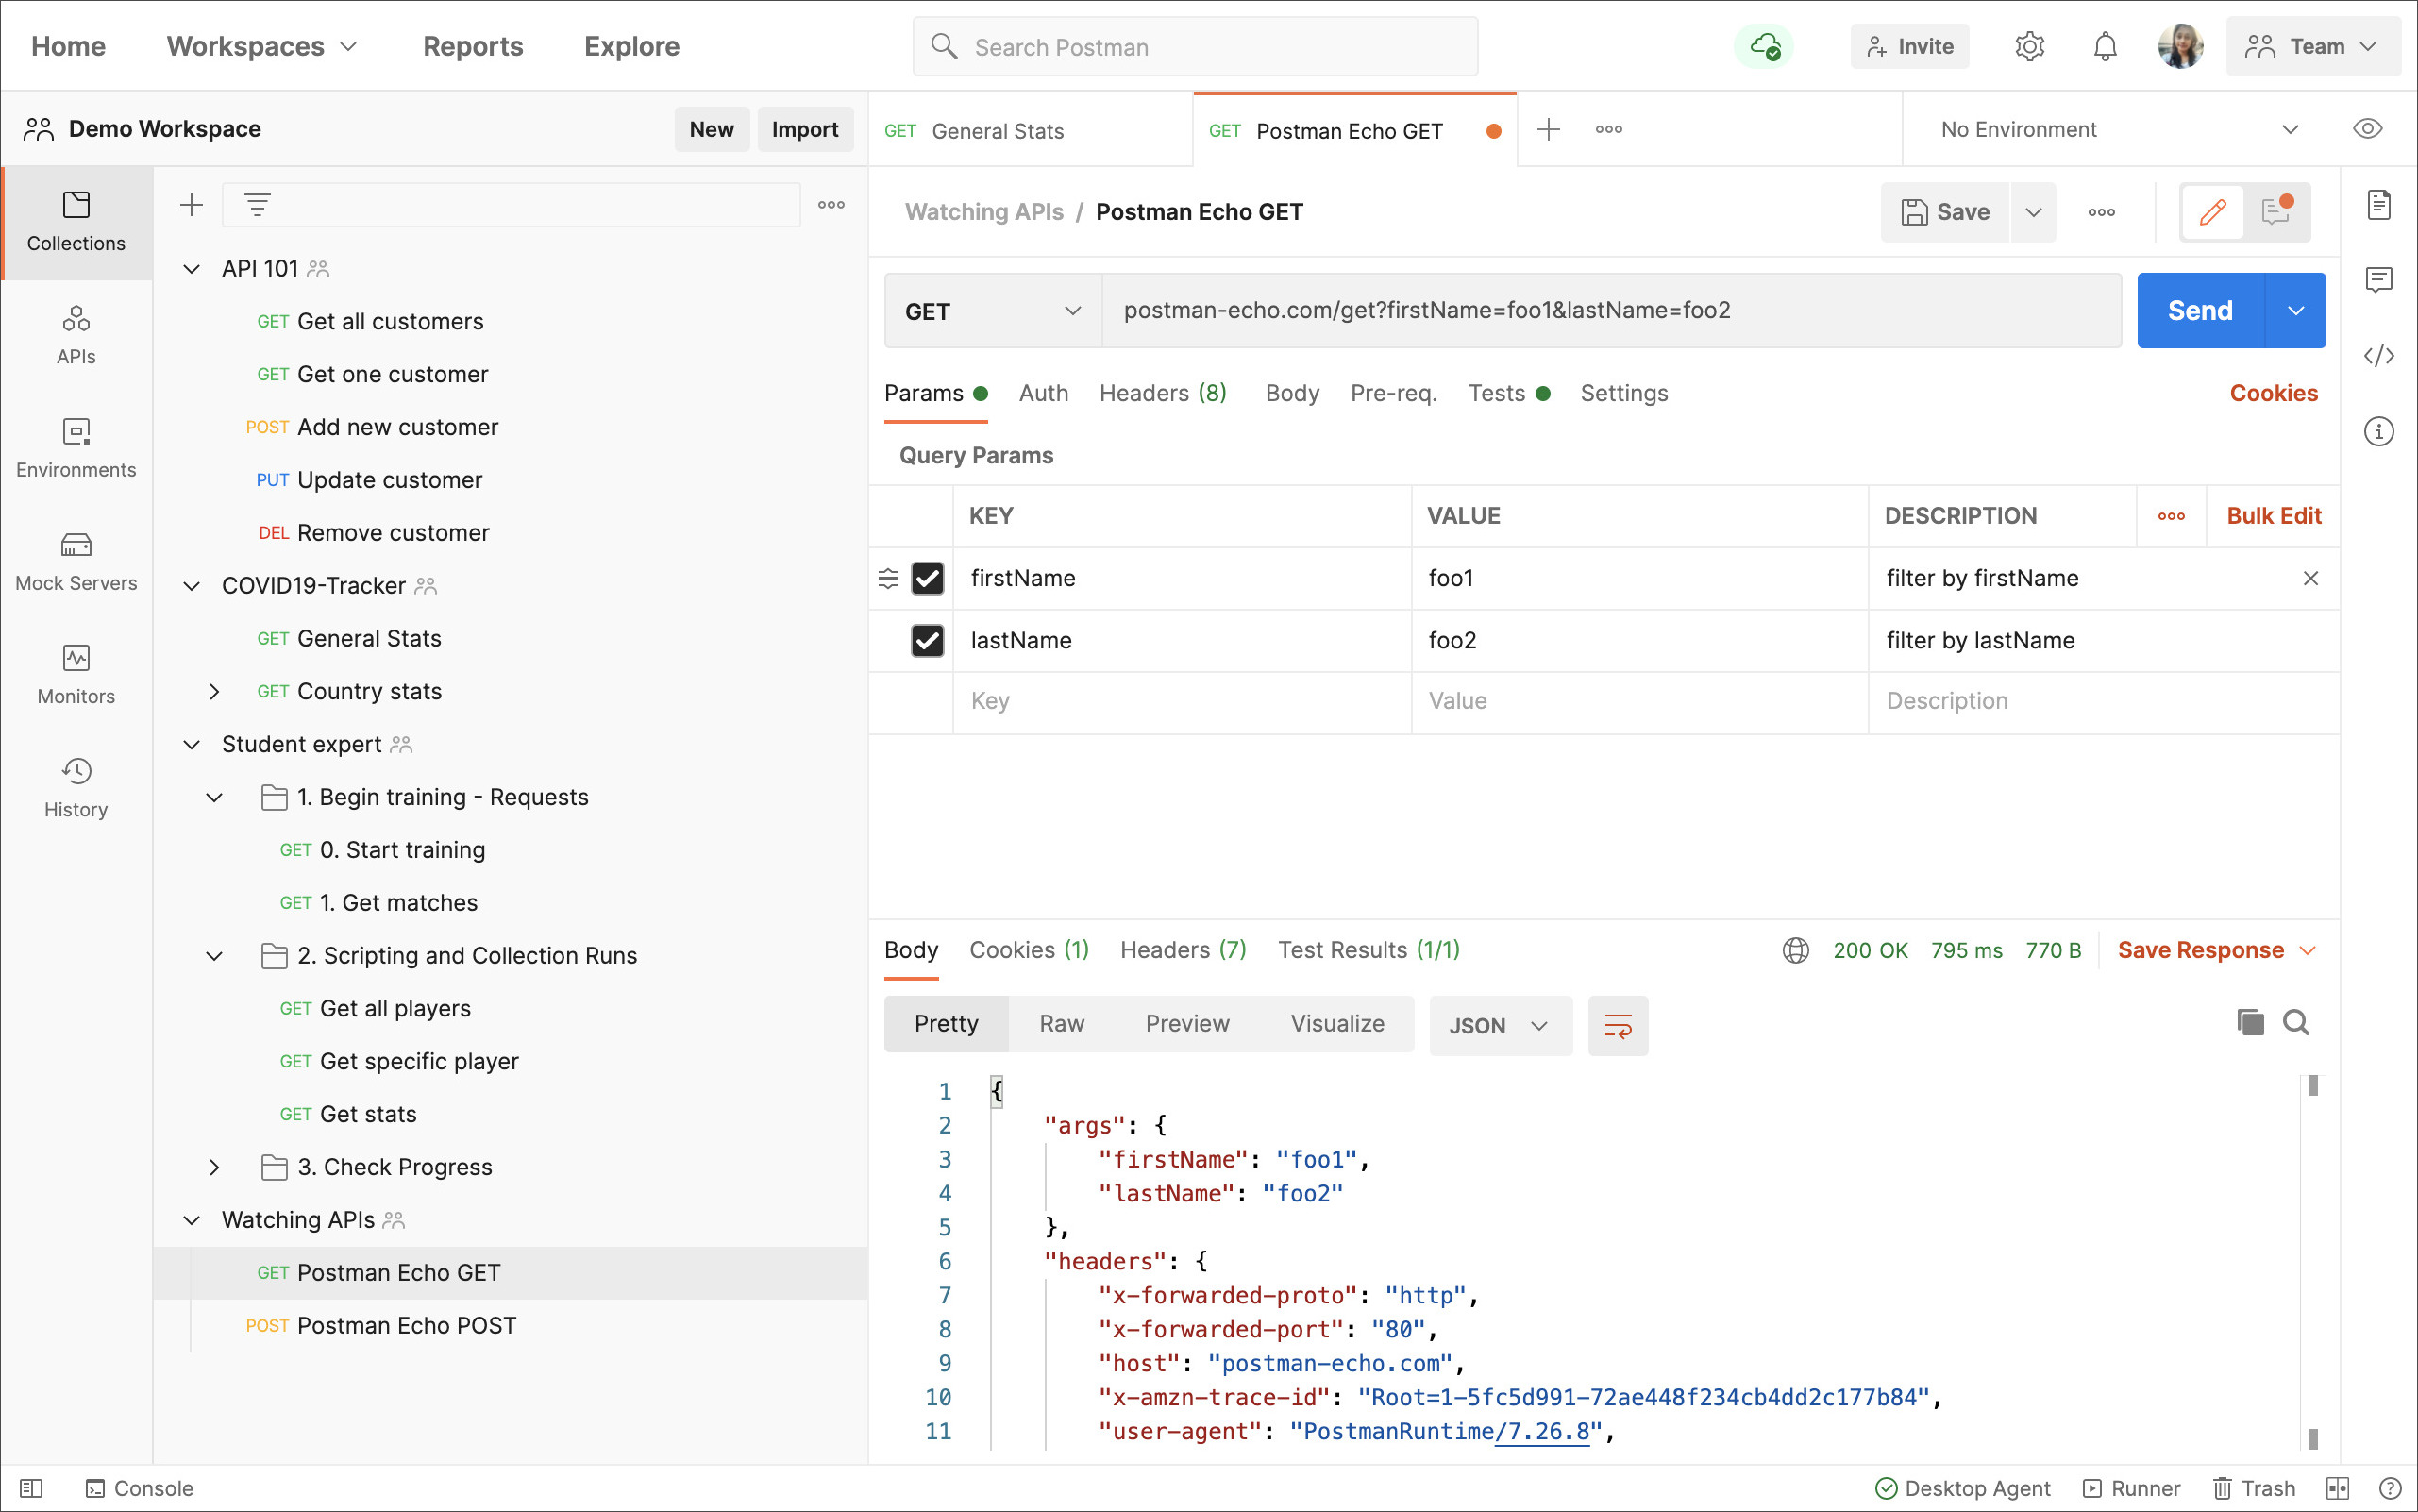
\includegraphics[width=1.0\textwidth]{final-year-project-template-master/img/postman.jpeg}
     \caption{Postman Endpoint test}
\end{figure}


 \subsection{Android Studio  Debugger}


Android Studio  Debugger - Kotlin Testing  : Android studio provides  a suite of tests at the time of compilation.The Debugger have a facility for  break points ,  window frames and watch-points which  helped shaped the quality of the application


 \subsection{Deployment test}
 I complied an Apk version of my application for testing on a standard Samsung android device to make sure the user interface , network access and screen rendering were operating correctly.Displayed below are images of the  application running.
 


 
 \begin{figure}[H]
  \centering
  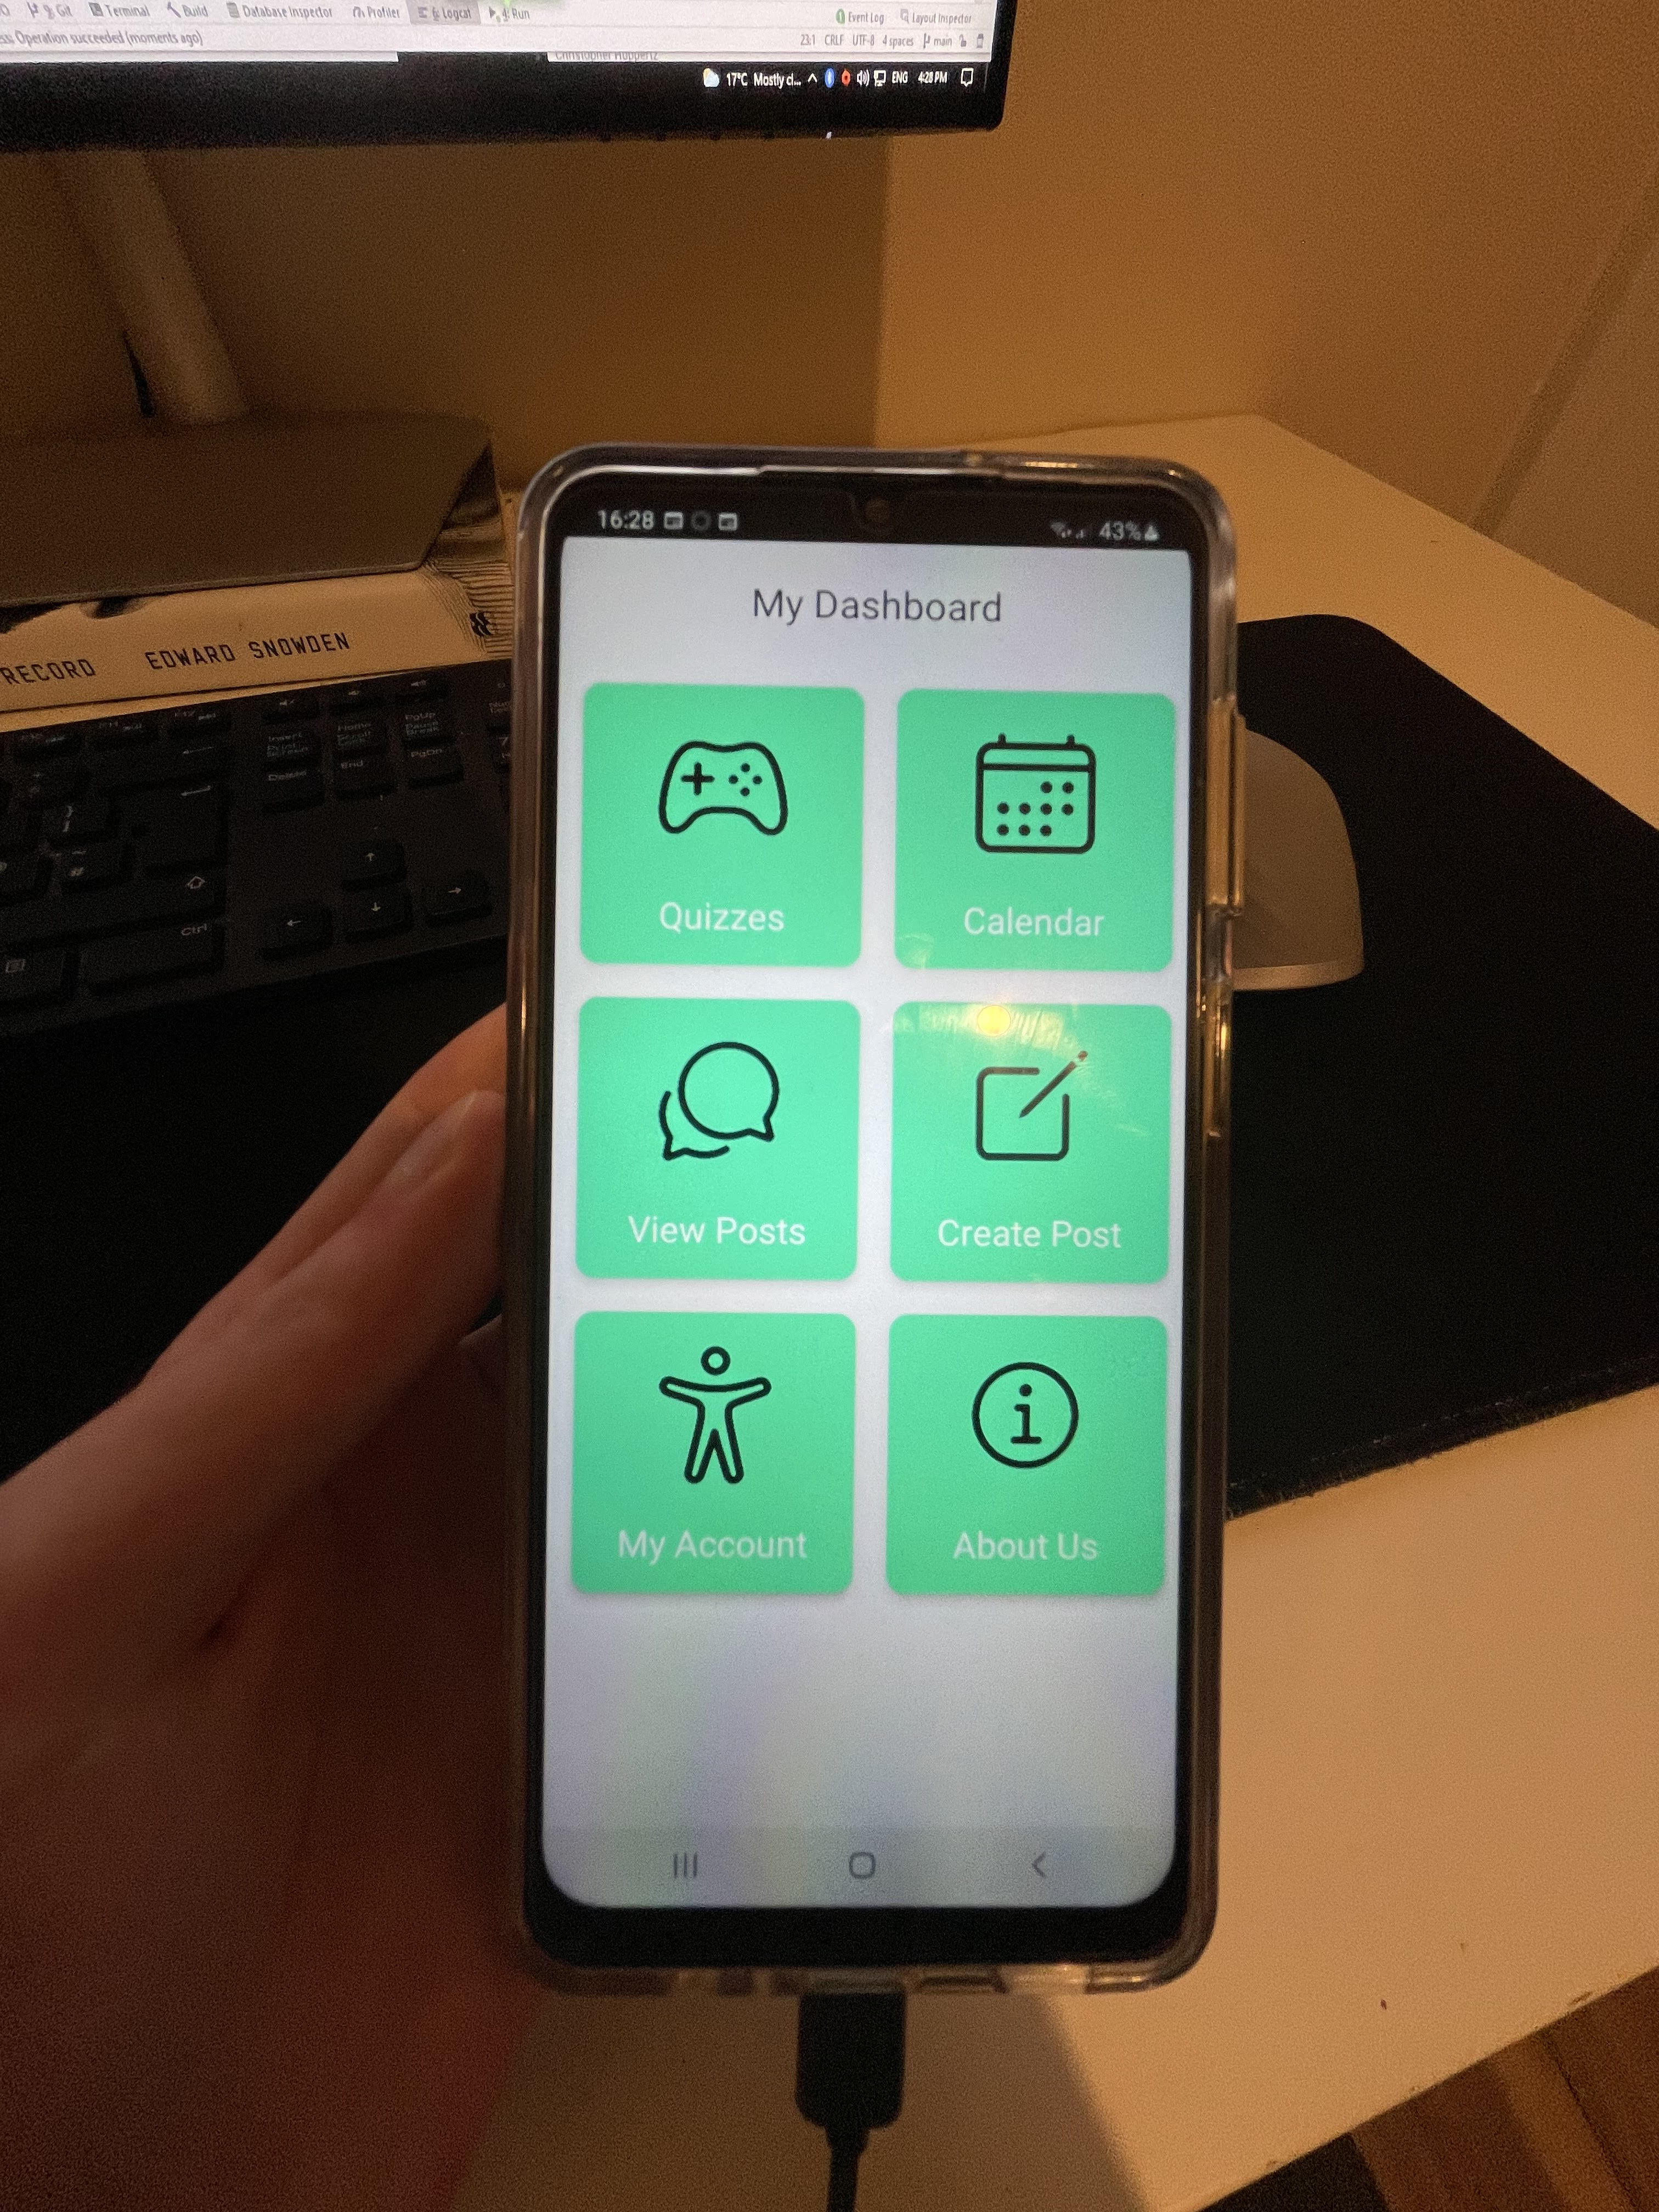
\includegraphics[width=0.25\textwidth]{final-year-project-template-master/img/onlinedash.jpg}
    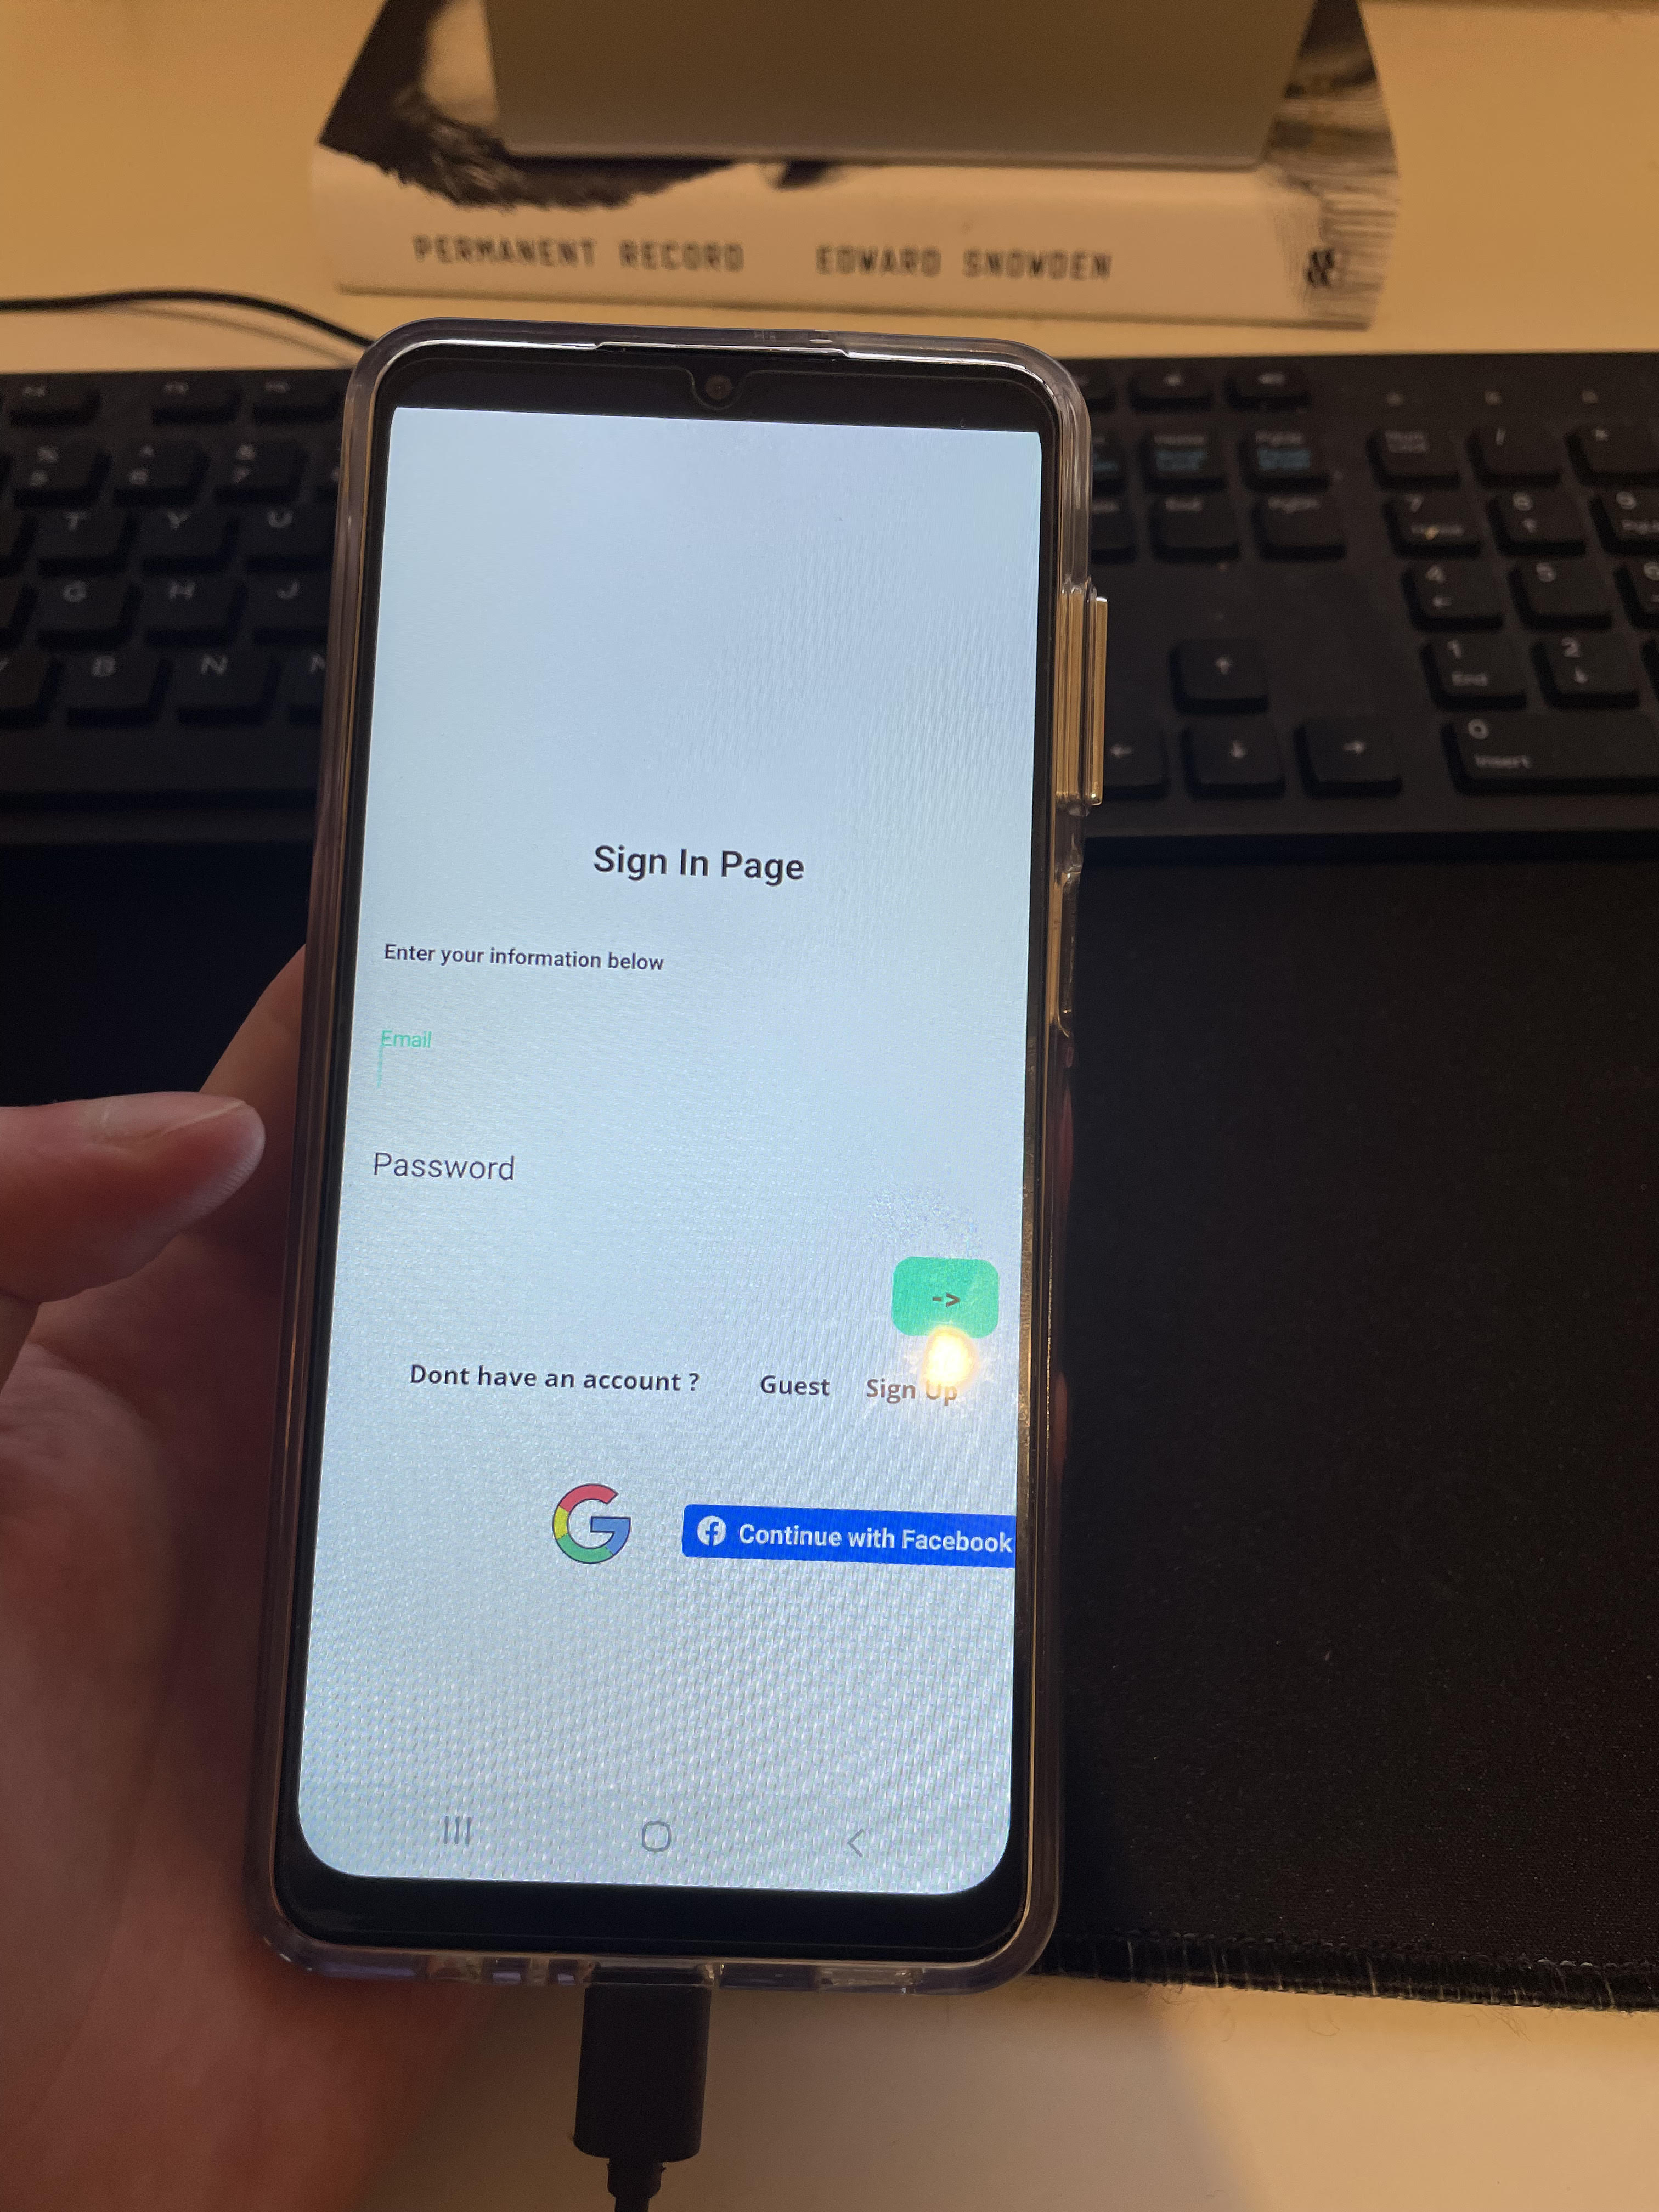
\includegraphics[width=0.25\textwidth]{final-year-project-template-master/img/homescreenonline.jpg}

     \caption{User Sign In and Dashbaord}
\end{figure}



 \begin{figure}[H]
  \centering
  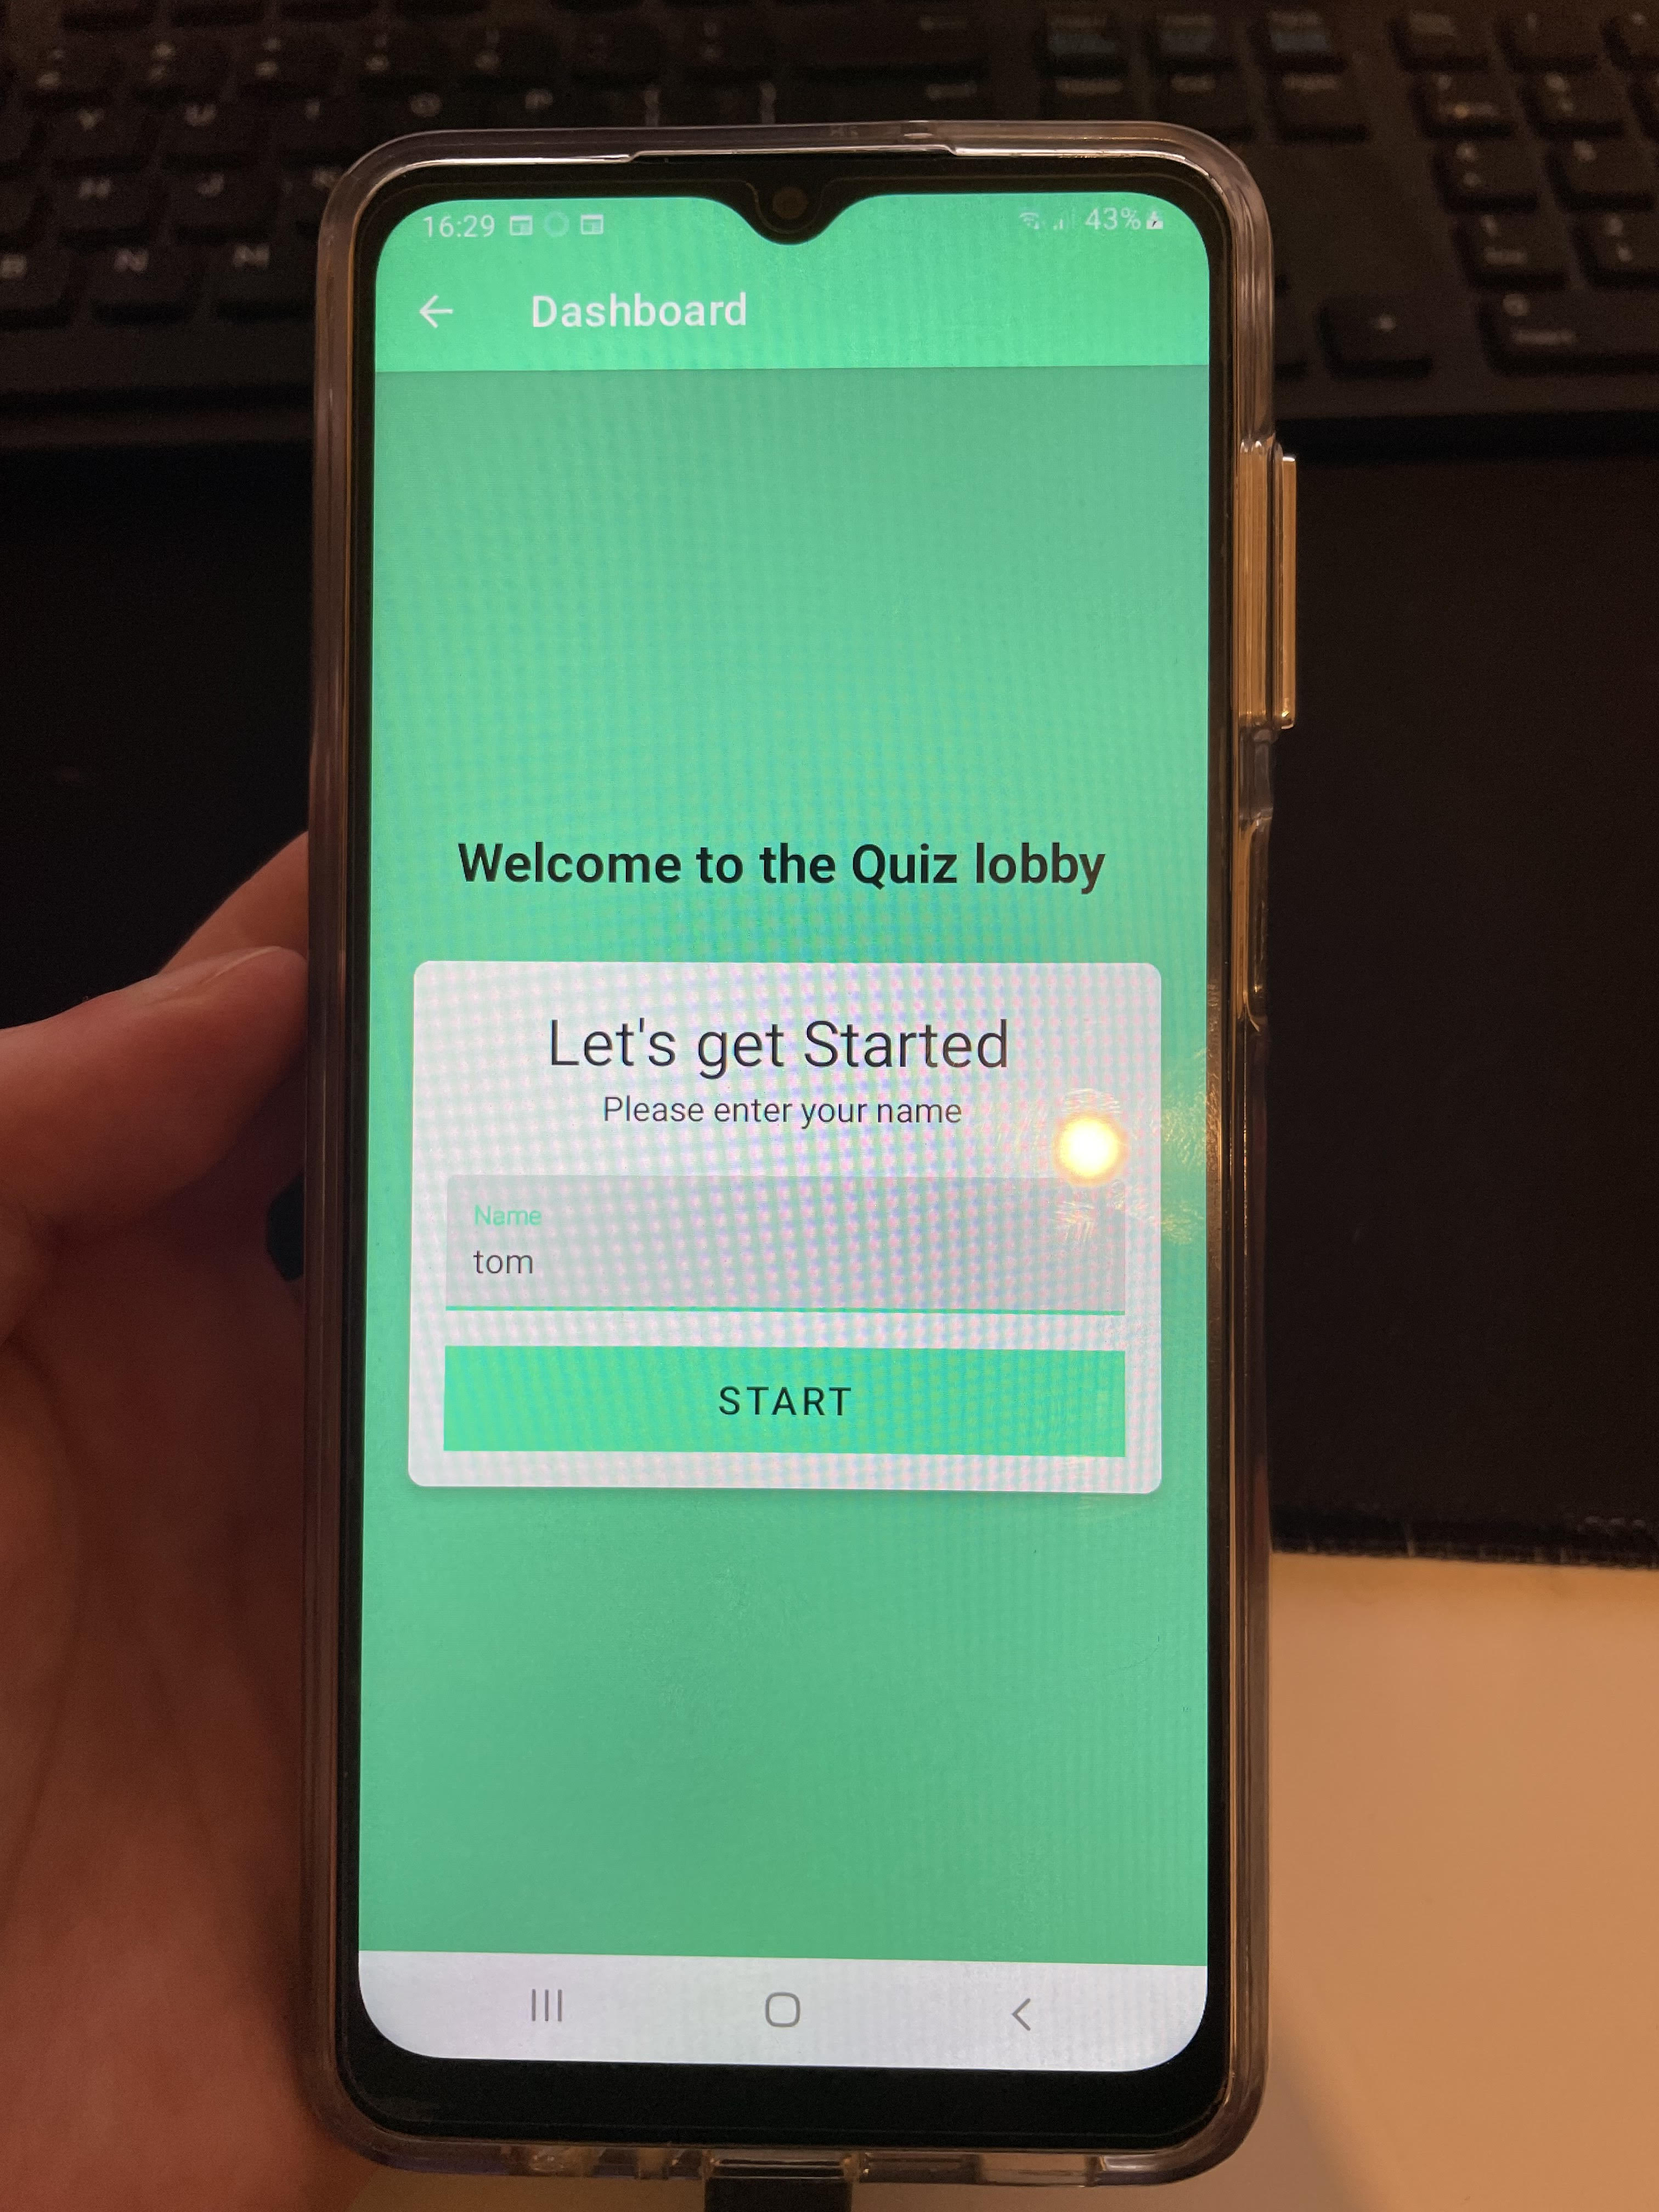
\includegraphics[width=0.25\textwidth]{final-year-project-template-master/img/lobby.jpg}
    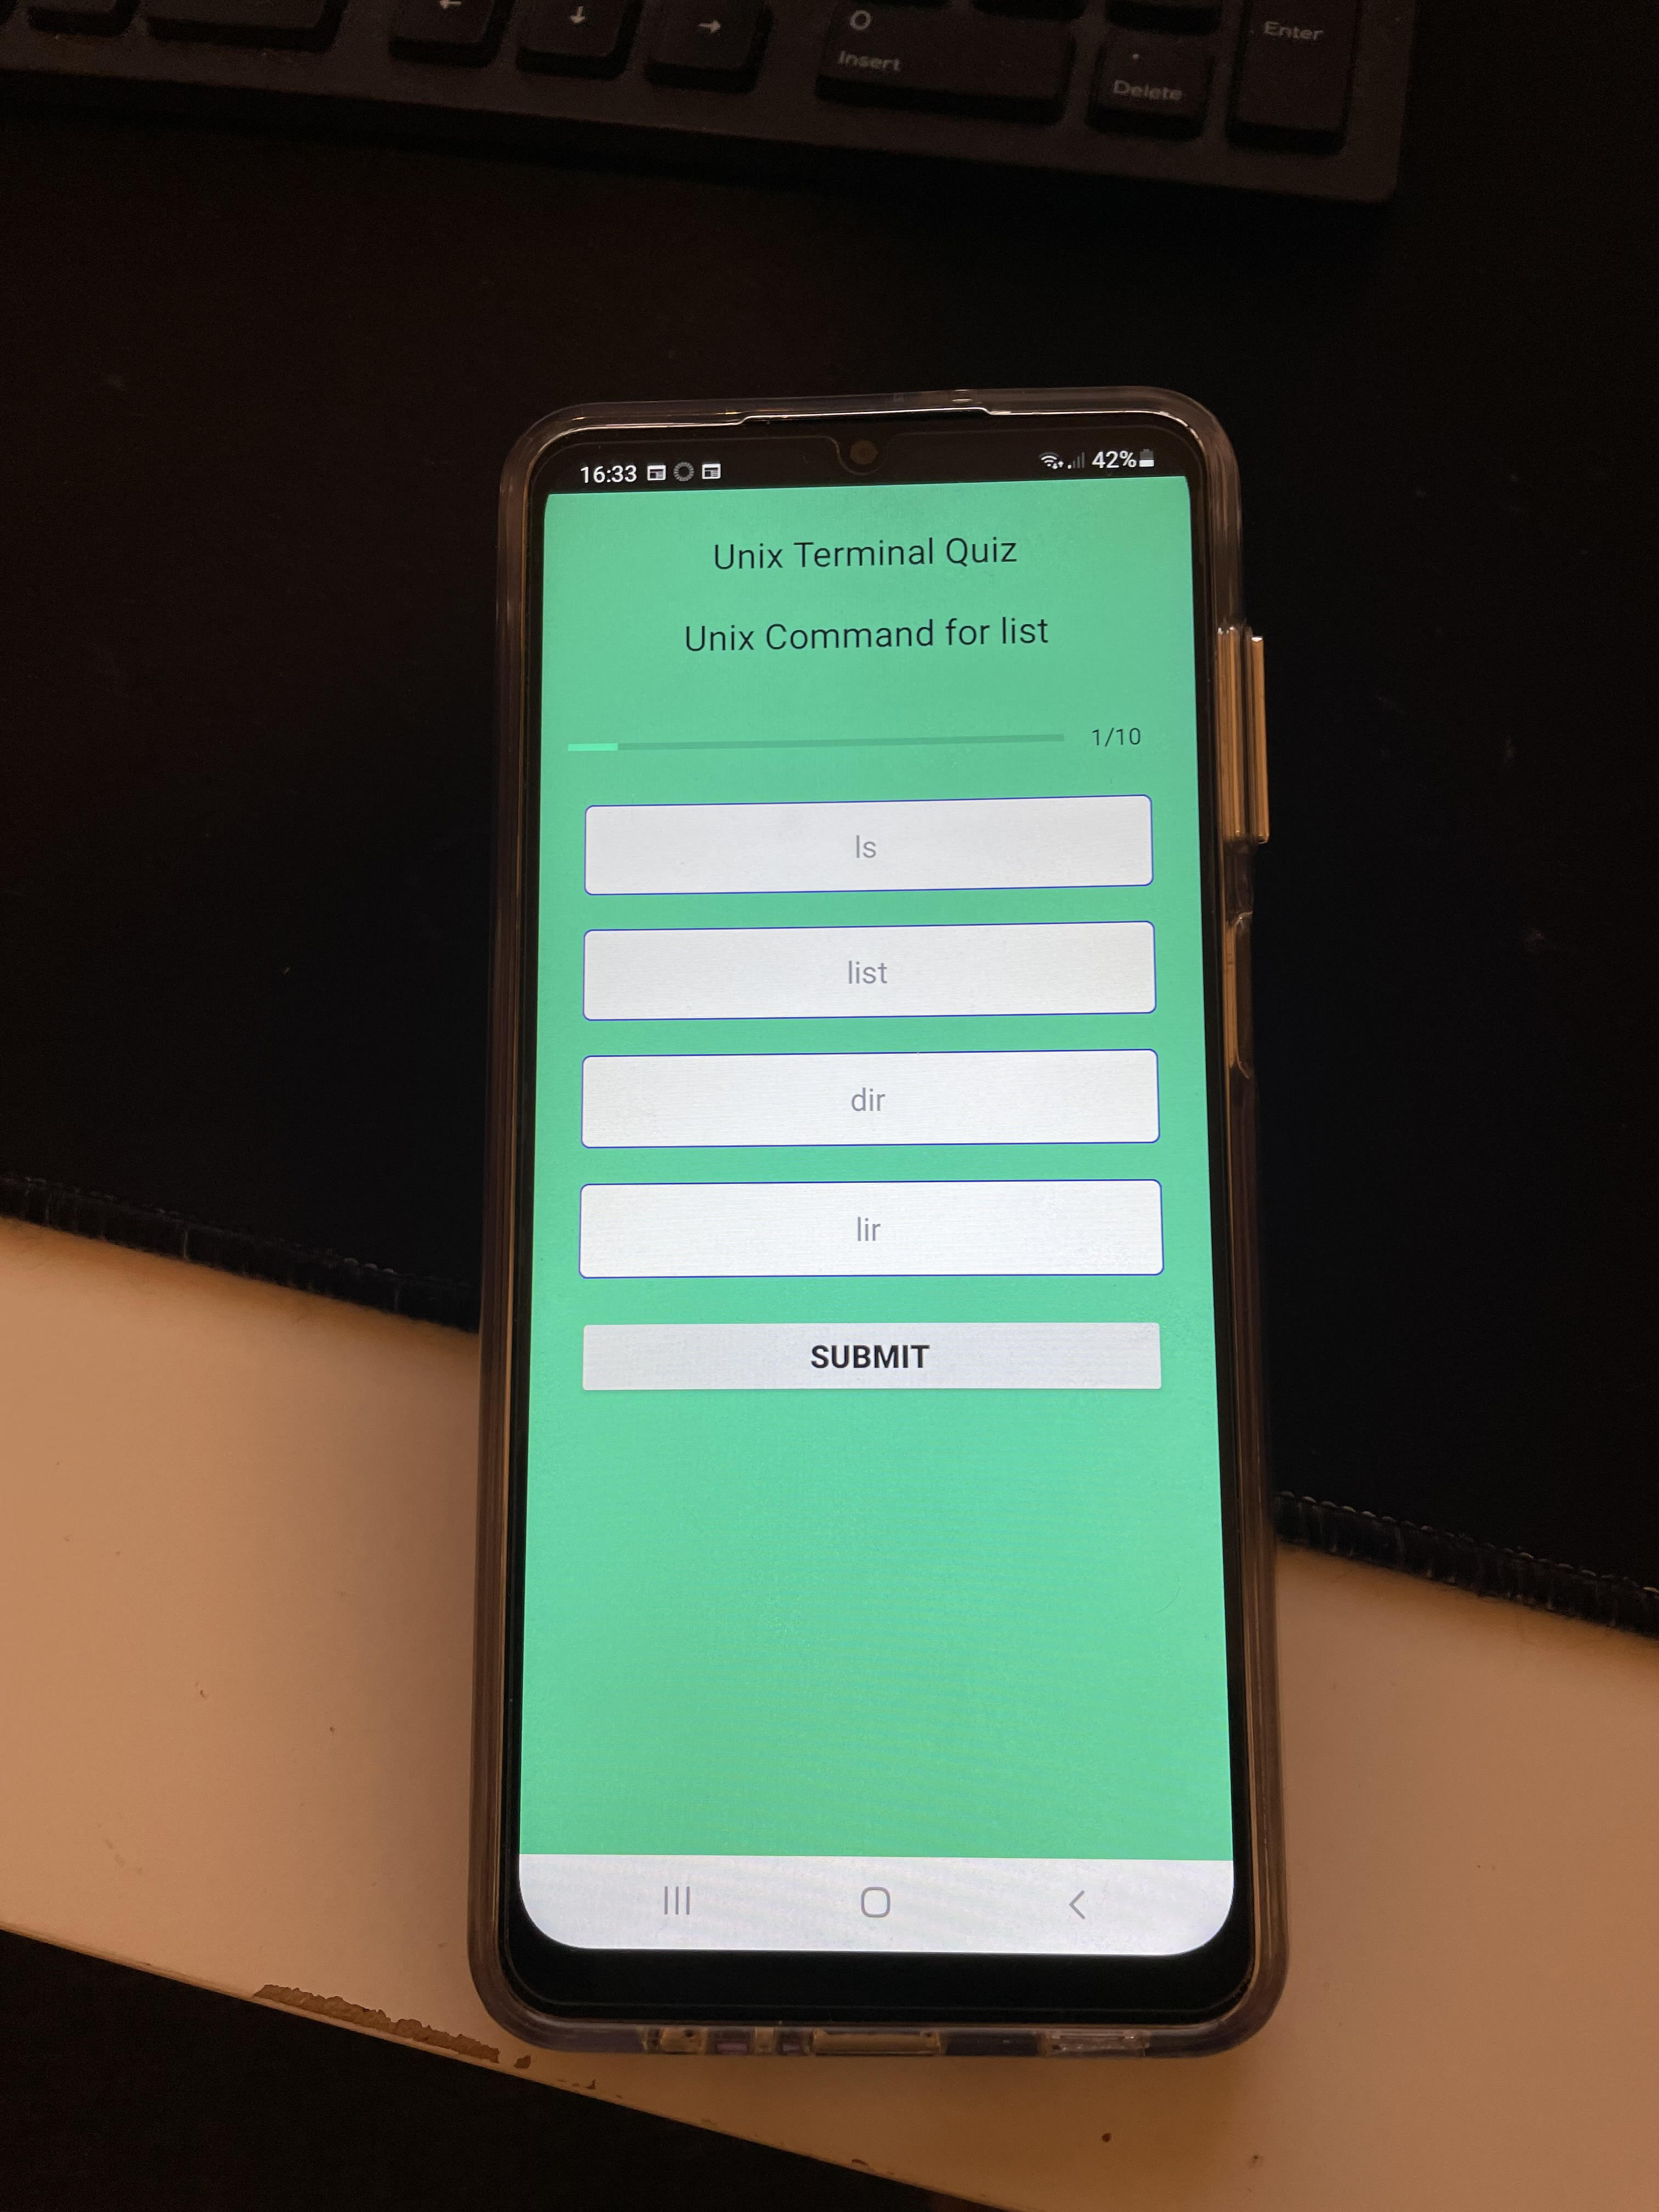
\includegraphics[width=0.25\textwidth]{final-year-project-template-master/img/questions.jpg}

     \caption{User Lobby and Quiz}
\end{figure}



\subsection{Client Evaluation}
Client-side refers to operations that are performed by the client in a client–server relationship in a computer network.
When evaluating the technologies for the project there were many considerations about the client side of the application. From early development, it was established that the user should be able to navigate the application without needing to read instructions. A good Human User interface is extremely important and I followed the Apple Human Interface Guidelines. Smartphones make up for 52 percent of traffic and it is vital to make an application as easy as possible to use.


\subsection{Server Evaluation}
Server-side refers to operations that are performed by the server in a client–server relationship in a computer network.
During the planning phase of the application I compiled a list of the most common server/back-end .Throughout my years of study I have worked with various  technologies such as JavaScript , MongoDB etc  for this application I needed a robust and agile platform and I decided on Node JS  due to its simple compile  and broad support.Node JS  is used  for many sites including PayPal which is one of the largest e-commerce  websites.
 

\subsection{Performance}
Android studio provides a well-featured environment for development.A  benefit is the 'Android Pro-filer' which allows developers to. monitor the performance of their application. Android Studio is developed by Intellij a widely used and successfully Java Enterprise Development Environment. Other tools applicable for development are as follows


\begin{itemize}
  \item Eclipse Java  IDE :  an integrated development environment used in computer programming. It contains a base work-space and an extensible plug-in system for customizing the environment.
  \item BlueStacks Android Emulator suitable for deploying android developed mobile applications.
  \item Xamarin : UWP  is an Open-source mobile app platform for .NET programmers.
  
  \item Xcode : Swift is a robust and intuitive programming language created by Apple for building apps for iOS, Mac, Apple TV and Apple Watch. It's designed to give developers more freedom than ever. Swift is easy to use and open source. 
\end{itemize}

A  benefit of the  Android studio IDE is its ease of use of software.The environment incorporates an android emulator for the developer to check the  programs behaviour 

\subsection{Overall  Evaluation}

This project has the  architecture as outlined  below  :

As shown above here is an outline of the technologies studied and implemented to create my application :

Kotlin , Node JS , Firebase , Heroku Cloud Deployment Development and  MongoDB

\begin{itemize}

\item Log In procedure for new user base.Underneath is the flow chart of the program once the user enrolls or attempts to enroll into the system.

 \begin{figure}[H]
  \centering
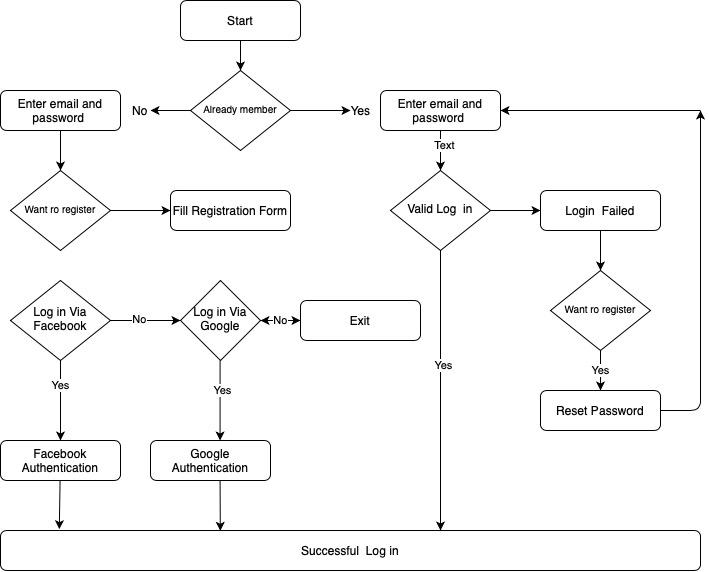
\includegraphics[width=1.0\textwidth]{final-year-project-template-master/img/Flowchart.jpg}
\caption{User Log In Flowchart}
\end{figure}



\item Database Systems in place.For the project I  incorporated the no-SQL approach using mongoDB to provide strong security and scaling for my program.

\href{https://medium.com/@rsk.saikrishna/when-to-use-mongodb-rather-than-mysql-d03ceff2e922}{MongoDB} 

\end{itemize}


\chapter{Conclusion}

\subsection{Overview}

I aimed to develop an electronic learning mobile application and there have been many hurdles and issues which I had to overcome.Defining a methodology early at development is essential to ensure a smooth experience for developers.In this section I will evaluate the goals set at the beginning before development.




 \subsection{ Review of Project Aims}
Here I will evaluate/review  the aims I set at the beginning of my project
 
     \begin{itemize}
     \item Create a strong and robust  three tier full stack  application.

     \textbf{PASS}
         \end{itemize}
         
         
          \begin{itemize}
     \item Create online Quiz

     \textbf{FAIL}
         \end{itemize}
         
          \begin{itemize}
     \item Evaluate/Research the current state of electronic learning.

     \textbf{PASS}
         \end{itemize}
         
         
          \begin{itemize}
     \item Deploy a full three tier stack to the cloud.

     \textbf{PASS}
         \end{itemize}
         
         
         
          \begin{itemize}
     \item Learn and implement the Kotlin language.

     \textbf{PASS}
         \end{itemize}
         
         
         
          \begin{itemize}
     \item Develop a clean user interface.

     \textbf{PASS}
         \end{itemize}
         
         
    
     
       \begin{itemize}
     \item Implement the agile methodology to plan and the control the progress of my Application.

     \textbf{PASS}
         \end{itemize}
     
     

\subsection{Project Outcome}
Throughout the duration of the project, I attempted to deliver weekly a piece of code or a documentation.The outcome was ultimately as expected but as this was a solo effort,  time management  was always a concern and is perhaps an underrated skill that is required  to become an effective software Developer.

\subsection{Discoveries}

During the beginning phase of development I used the Ruby on Rails framework.After a month of development it became clear from bugs/issues the application was too complicated to design using a web approach.After researching I settled on my application as a  mobile application   rather than  web application as initially intended.


\subsection{Managing a Full Stack Application }
The most difficult part of creating this application was integrating  its full stack architecture.Kotlin is a decade old language and does not have as much documentation as much more mature languages such as C , Java etc.I relied on documentation from third party rest client tutorials such as OK-HTTP and retrofit.Delegating time equally between the front and back-end elements was difficult due to the alternative syntax between JavaScript and Kotlin and XML.GitHub version controls bot which automatically updates packages created issues with my code-base which resulted in wasted time spent debugging references to packages.


\subsection{Application Limitations}


 \begin{itemize}
     \item \textbf{App scaling:} An issue with Android studio is the scaling of the application.Android studio forces developers to deploy to one specific screen ratio.I chose the Google Pixel as it is one of the most popular devices.Without any  tool equivalent  to Bootstrap for web applications, this means that the user experience will vary for user and create inconsistencies.There are over  1,300\cite{totalbrandandroid} android brands which share different aspect ratios on screen resulting in a different experience for users.This isnt a common issue on Apple devices as there are less than 30 unique devices on the market.
     
     \item \textbf{Missing Platforms:} Currently the application is  supported by the Android Platform meaning users using the Apple mobile OS 'iOS' will not be able to use my application.I hope to create a build for iOS at a later stage.The application can be ported to the iOS platform .
     
     \item \textbf{Speed:} The speed of the application for replies on the users network speed and mobile hardware( CPU , GPU) . I encountered issues with crashes using the OKHTTP and Retrofit while  making requests towards the Heroku server.One possible solution to this issue is to upgrade the server hardware which is a feasible option if the application generated revenue.
     
         \end{itemize}
         
\subsection{Reflection}
Overall I am proud of the project I developed. Developing and maintaining a full-stack code-base was an extremely difficult task but has helped me become a more educated and experienced programmer. Learning a new programming language was overwhelming during early development but already having experience with design patterns, database systems helped me immensely. I felt working remotely to be a strenuous task but has given me an insight into how companies collaborate while not in the workplace. Efficient research proved to be an essential tool for development, Android provides effective and detailed documentation for development. I was disappointed I could not store the quiz questions inside a database scheme, I opted for local storage, this is a feature that caused great issues. I hope to add more to this project in the future and deploy it to the public android store. Time management and research have proven to me from this experience to be vital elements to develop within a time frame and to maintain a level of quality consistently throughout the application. I would like to thank my supervisor, Dr. John French, for his judgment on how to create a well-structured application and dissertation.
\chapter{ Appendices}


\subsection{GitHub Link}

\begin{itemize}

\item \textbf{Link to GitHub Repository} 
\item https://github.com/OmalleyFinalYearAppliedProject/FinalYearAppliedProjectGMIT
\end{itemize}

\subsection{Run Mobile App locally}


\begin{itemize}
\item git clone 
\item https://github.com/OmalleyFinalYearAppliedProject/FinalYearAppliedProjectGMIT.git
\item Install and Open Android Studio Application
\item cd FinalYearAppliedProjectGMIT
\item build
\item Download apk and deploy to Android Device or Build for Emulator.
\end{itemize}

\subsection{Run Web Server locally}

\begin{itemize}

\item git clone 
\item https://github.com/OmalleyFinalYearAppliedProject/FinalYearAppliedProjectGMIT.git
\item Install Node
\item cd quiz-backend/src
\item  npm start server.js
\end{itemize}

\subsection{Access Server via Browser}
\begin{itemize}
\item https://dashboard.heroku.com/apps/quiz-node-js-backend
\end{itemize}
